\part{L’IA et les données patrimoniales, les musées et institutions publiques à l'heure de l'accélération numérique}

%%%%%%%%%%%%%%%%%%%%%%%%%%%%%%%%%%%%%%%%%%%%%%%%%%%%%%%%%%%%%%%%%%%%%%%%%%%%%%%%%%%%
%%%%%%%%%%%%%%%%%%%%%%%%%%%%%%%%%%%%%%%%%%%%%%%%%%%%%%%%%%%%%%%%%%%%%%%%%%%%%%%%%%%%
%%%%%%%%%%%%%%%%%%%%%%%%%%%%%%%%%%%%%%CHAPITRE%%%%%%%%%%%%%%%%%%%%%%%%%%%%%%%%%%%%%%
%%%%%%%%%%%%%%%%%%%%%%%%%%%%%%%%%%%%%%%%%%%%%%%%%%%%%%%%%%%%%%%%%%%%%%%%%%%%%%%%%%%%
%%%%%%%%%%%%%%%%%%%%%%%%%%%%%%%%%%%%%%%%%%%%%%%%%%%%%%%%%%%%%%%%%%%%%%%%%%%%%%%%%%%%

\chapter{Les humanités numériques au service du patrimoine}

Face à la numérisation croissante du patrimoine, son accessibilité en ligne et les nouvelles opportunités offertes par les traitements automatisés, les institutions patrimoniales et les chercheurs en sciences humaines se mobilisent depuis plusieurs années déjà pour concevoir des infrastructures et des réseaux de recherche efficaces pour répondre aux problématiques nouvelles auxquelles ces outils permettent de répondre. Avant d'aborder les procédés que nous avons spécifiquement entrepris dans le cadre du stage au sein du département des Arts graphiques, nous voulons proposer un tour d'horizon des projets actuels et des structures en place qui poussent au quotidien pour une meilleure appréhension des outils automatisés et d'intelligence artificielle au sein des sciences humaines.

Une partie non-négligeable du stage a été de faire le lien avec plusieurs groupements de recherche et institutions, que ce soit pour communiquer à propos du projet TORNE-H ou bien nourrir la réflexion du projet en assistant à divers événements et conférences. 

\section{Les acteurs de la recherche en sciences humaines computationnelles}

En 2025, une galaxie d'institutions et de groupements prennent part aux développements récents en humanités numériques en France. Ce ne sont pas seulement des institutions publiques, comme des institutions patrimoniales, des Consortiums de recherche, ou des laboratoires. On trouve aussi des entreprises privées et des EPIC (Établissement public à caractère industriel et commercial). Dans le premier cas, il s'agit de l'entreprise Teklia, avec laquelle nous avons pu collaborer, et dans le second de l'Institut National de l'Audiovisuel. D'un côté Teklia propose des solutions technologiques pour la reconnaissance de texte (OCR/HTR), l'extraction d'information, l'analyse de la structure et la classification de documents. De l'autre, l'INA, en plus de remplir sa mission de collecte du paysage audiovisuel français, propose un certain nombre d'approches innovantes à la croisée entre sciences sociales et méthodes computationnelles afin de traiter de l'immense corpus qu'ils ont à disposition. Ensuite, nous avons aussi des acteurs universitaires comme les laboratoires de recherche, notamment l'Institut de Recherche et d'Histoire des Textes, le Médialab à Sciences Po, le Centre Jean Mabillon à l'École des chartes ; mais aussi l'INHA, le CERES de Sorbonne Université, et le Centre Internet et Société du CNRS. Enfin nous avons aussi des institutions comme les Maisons des Sciences de l'Homme, en soutien à la recherche ou bien la BNF. Tous ces acteurs, en grande partie des acteurs publiques, collaborent souvent, entretiennent des listes de diffusions communes, et forment des groupements pour soutenir leurs visées de recherches.

\subsection{L'environnement de recherche de TORNE-H}

Dans le cadre du partenariat de recherche dans lequel s'inscrit le projet TORNE-H, nous sommes sous l'égide du Consortium Huma-Num PictorIA. Cet acronyme veut dire \enquote{Programme d'identification, classification, traitement d'images, observation et reconnaissance des formes par l'intelligence artificielle}. Ce Consortium réunit une partie des institutions que nous avons citées plus haut : l'INA, la MSH Mondes, l'INHA, la BNF, l'École des chartes, mais aussi La contemporaine. Il est sous la tutelle du CNRS, de l'Université Paris 1 Panthéon-Sorbonne et de l'Université Paris Nanterre. Il est \enquote{dédié à l’analyse de corpus visuels numériques en sciences humaines et sociales par le biais d’outils d’intelligence artificielle}\footnote{\cite{noauthor_pictoria_nodate}}.

Le Consortium se structure autour de deux axes principaux: un axe « Traitement et exploration de données » et un axe « Diffusion ». Ces axes sont répartis d’une part en groupes de travail experts (GT), qui se concentrent sur des tâches précises afin de produire des livrables à forte valeur technique (jeux de données, développements, plateformes d’analyse, modèles préentraînés, tutoriels) et peuvent agir en support des autres groupes; d’autre part, en communautés de pratique (CP), centrées autour d’enjeux disciplinaires, qui testent les outils sur des corpus précis, en dialogue avec les ingénieurs, et développent des protocoles susceptibles d’être reproduits\footnote{\cite{noauthor_groupes_nodate}}. \hfill \break

L'initiative est adossée à l'Infrastructure de Recherche (IR*) Huma-Num qui est une infrastructure de recherche nationale pionnière dans le domaine des SHS computationnelles et de la mise en œuvre de l'ouverture des données et de l'interopérabilité au sein de la recherche en France. Huma-num est lancé depuis 2013 et \enquote{propose un ensemble de services et d'outils pour les données numériques produites dans les projets de recherche en Sciences Humaines et Sociales. Ces services et outils sont construits sur un ensemble de technologies d’infrastructure (serveurs) et de systèmes informatiques mis à la disposition des laboratoires et équipes de recherche pour mutualiser, diffuser et stabiliser l’accès aux données et documents.}\footnote{\cite{noauthor_presentation_nodate}}. 

L'infrastructure mène des actions d’expertise, participe à la conception de guides de bonnes pratiques, de formations, de plateformes de données ancrées dans les Maisons des sciences de l’homme. Elle s’appuie sur les moyens de centres de calcul nationaux (centre de calcul de l’CNRS Nucléaire et Particules, CINES). Elle coordonne la participation de la France dans les infrastructures européennes DARIAH ERIC et CLARIN ERIC. Dans le cadre du Consortium c'est notamment grâce à Huma-Num que nous avons accès à des solutions de stockage à long terme et aux services de l'entreprise Teklia et de sa plateforme Arkindex.

\subsection{La collaboration autour de la vulgarisation d'outils au sein du Consortium}

Durant le stage, nous avons animés le Groupe de Travail (GT) Formation et Animation du Consortium PictorIA, nous avons menés une mission coordonnée de partage d'information et de formation à destination des membres du Consortium. Sous la supervision de Julien Schuh, coordinateur scientifique de PictorIA, avec Fantin Le Ber, stagiaire à la MSH Mondes de Nanterre et Pierre Husson stagiaire à l'INHA nous avons appris à prendre en main le \textit{workflow orchestrator} Arkindex de la société Teklia\footnote{\cite{noauthor_quest-ce_2025}\enquote{\textit{Alors que l’automatisation des workflows consiste à automatiser les tâches individuellement, l’orchestration des workflows crée un écosystème au sein duquel ces tâches automatisées interagissent efficacement, suivent une séquence logique et s’intègrent à d’autres systèmes pour former un processus métier de bout en bout}}.}. La société collabore avec PictorIA dans le cadre de l'infrastructure de recherche Huma-num et possède une instance et des modèles dédiés pour la mise en place au sein de projets de recherches d'opérations d'OCR, de détection d'objets, de \textit{layout recognition\footnote{\textit{cf}. le \textbf{\hyperref[sec:Glossaire]{Glossaire}}, p.~\pageref{sec:Glossaire}.
}}, etc,. 

Ces séances de travail ont amenées à la rédaction de deux tutoriels et à la tenue de deux journées de formation à destination des institutions partenaires du Consortium comme le Datalab de la BNF, l'INHA, la MSH Mondes, ou le CNRS\footnote{\textit{cf}. l'\textbf{\hyperref[sec:Formations]{Annexe E}}, p.~\pageref{sec:Formations}.}. La première s'est tenue le 23 juin 2025, et nous avons mis à disposition des jeux de données contenant des numérisations de presses du \textsc{xix}\textsuperscript{e} siècle et des peintures italiennes\footnote{\cite{le_ber_tutoriel_2025-1}.}. L'idée était de guider pas à pas des publics peu ou pas habitués à la programmation dans le processus de traitement automatisé. Pour cela nous avons configurés des \enquote{\textit{workers}} avec certaines tâches spécifiques comme l'OCR, la description d'image par un LLM ou la reconnaissance de mise en page pour faire tester les processus\footnote{\textit{cf}. le \textbf{\hyperref[sec:Glossaire]{Glossaire}} pour les termes \enquote{LLM} et \enquote{\textit{layout recognition}}, p.~\pageref{sec:Glossaire}.}. L'idée derrière cet outil est de pouvoir chaîner les \textit{outputs} d'une ou plusieurs opérations comme \textit{input} d'une autre opération. Cela permet par exemple de faire passer un modèle de reconnaissance de mise en page, d'envoyer le résultat du processus dans un \textit{worker} qui fait de l'OCR, qui va lui-même envoyer le résultat dans un algorithme de Reconnaissance d'Entités Nommées. La seconde journée va se dérouler le 18 septembre à la MSH Mondes de Nanterre sur le même principe\footnote{\cite{schuh_seminaire-atelier_2025}}.

Dans le cadre de la préparation de ces journées nous avons été en contact avec le directeur de Teklia, Christopher Kermorvant et Bastien Abadie, directeur technique chez Teklia, qui ont pris le temps de répondre à nos questions pour nous permettre de préparer au mieux les formations. Cela nous a permis aussi de faire remonter des cas d'usages et des demandes spécifiques aux enjeux de recherche que nous rencontrons dans le cadre de nos stages afin d'affiner, de concert avec la société, l'offre du \textit{workflow orchestrator}. 

\section{Les projets de recherches actuels}

Dans cette section nous voulons revenir sur les projets de recherche en cours au sein du Consortium, et évoquer rapidement les participations du projet à la diffusion de la recherche. Les projets de recherches que nous évoquons nous semblent mettre en œuvre ou explorer des problématiques identiques, ou très similaires, à celles que le musée pourrait rencontrer dans la perspective du traitement des collections. 

Tout d'abord, dans le cadre du projet TORNE-H nous avons eu l'opportunité, grâce aux financements du FTNC, de communiquer à plusieurs reprises dessus. Le 4 juillet, nous étions présent\wokisme e \wokisme s aux côtés d'Emmanuelle Bermès, qui pilote le projet au Centre Jean Mabillon, au Congrès PFIA de Dijon, où nous avons présenté les enjeux et avancées du projet. Le 30 septembre une journée d'étude est organisée au sein du musée afin de marquer la fin de la première année du projet. Enfin, le 14 novembre, l'équipe de TORNE-H sera présente au colloque DH Nord à Tourcoing organisé par la MESHS afin de présenter le résultat des expérimentations de la curation assistée par IA au musée. 

\subsection{HikarIA et le musée Guimet}

Pour ce premier projet, nous regardons du côté du Musée Guimet et de la collection Dubois qui y est conservée. Cette collection de photographies anciennes du Japon comporte 19 000 phototypes datant de l'ère Bakumatsu et Meiji (entre 1853 et 1912). Ces photos, à destination d'un public occidental, représentent des mises en scènes idéalisées et mises en couleurs à la main par des peintres japonais. Ce projet est coordonné par le conservateur des collections photographiques du musée et en collaboration avec l'entreprise Teklia et son président et directeur scientifique Christopher Kermorvant. Pour permettre le traitement par intelligence artificielle de la collection \enquote{l’adoption du protocole IIIF est devenue une norme, permettant un accès standardisé aux images et aux métadonnées\footnote{\textit{cf}. le \textbf{\hyperref[sec:Glossaire]{Glossaire}} pour le terme \enquote{IIIF}, p.~\pageref{sec:Glossaire}.}. Cette approche numérique permet la valorisation non invasive des images photographiques et améliore la gestion des collections, facilitant ainsi la réalisation d’études quantitatives approfondies}\footnote{\cite{saint-ours_de_projet_2024}. p. 21-22.}. 

En utilisant les avancées dans les modèles visuels d'apprentissage profond qui utilisent les \enquote{réseaux de neurones convolutifs et des modèles}\footnote{\cite{saint-ours_de_projet_2024}. p. 22.}, et en enrichissant les métadonnées descriptives, il a été possible de décrire et de faire catégoriser les 19 000 images du fonds en une base de données interrogeable en langage naturel sur le site \url{https://hikaria.org/search/}\footnote{\textit{cf}. le \textbf{\hyperref[sec:Glossaire]{Glossaire}} pour le terme \enquote{réseau de neurones convolutifs}, p.~\pageref{sec:Glossaire}.}. Si nous citons ce projet c'est parce qu'au gré d'une redécouverte dans les archives du MAD, dans le cadre d'un chantier de collection photographique sous la direction de Sébastien Quéquet, ont été retrouvés des albums de photographies japonaises datant de 1881 à 1913. Ces albums sont issus du Leg Gustave Schlumberger et du don Raymond Koechlin qui ont tous deux cédés au musée des albums du photographe japonais Kusakabe Kimbi, et le musée pourrait bénéficier d'un projet similaire de reconnaissance ou d'indexation automatique des images et de leur contenu. 

\subsection{Extraction et interprétation sémantique de tables anciennes}

Projet porté par le Centre de Recherches Historiques de l'EHESS, et présenté lors du Congrès PFIA de Dijon, il s'agit d'un projet d'\textit{Handwritten Text Recognition} sur des tables anciennes (l'HTR est l'équivalent de l'OCR mais sur l'écriture manuscrite)\footnote{\cite{tual_extraction_2025}}. L'idée de ce projet est de pouvoir extraire des tables historiques les informations pour pouvoir manipuler les données. Dans les archives il y a nombres de tableaux partiellement imprimés, partiellement remplis à la main, qui comportent des abréviations, des dépassements, des flèches, des bulles et autres variations qui rendent la lecture et la compréhension des tables compliquées pour un modèle automatique. Cependant, l'équipe derrière le projet a mis au point une chaîne de traitement qui associe des méthodes d'extraction d'informations et d'interprétation sémantique de tables à l'aide d'un graphe de connaissances pour pallier ces problèmes\footnote{\textit{cf}. le \textbf{\hyperref[sec:Glossaire]{Glossaire}} pour le terme \enquote{graphe de connaissances}, p.~\pageref{sec:Glossaire}.}. Ils utilisent un modèle DAN, mis en production par Teklia pour faire de l'extraction d'information sans segmentation préalable\footnote{\cite{noauthor_dan_nodate}}. L'intérêt de cette démarche est de pouvoir faire de la reconnaissance d'entités nommées par la suite et d'extraire les informations dans un format portable et facilement interrogeable.

Ce projet propose des outils et une réflexion très intéressante pour deux fonds sur lesquels nous avons pu travailler : les carnets de Paul Henrot et les carnets de Jean Royère. Dans les deux cas les structures des tables ne sont pas très complexes et pourraient bénéficier d'un traitement automatisé. Ceux d'Henrot comportent les noms de ses clients, les dates et les temps de développement de ses pellicules et une extraction des données pourrait permettre de cibler les bobines intéressantes que le musée pourrait faire numériser ou développer en vue d'une exposition. Dans le cas de Royère, ce sont ses carnets de clients et de commandes, avec les dates mais surtout avec les références des magazines dans lesquels apparaissent ses designs. Ce dernier point est très précieux parce que la plupart des magazines cités sont disponibles sur Gallica et un traitement de recoupement et d'enrichissement est envisageable, notamment pour reconstruire les couleurs des meubles et les remettre en contexte en les croisant avec les dessins et gouaches de l'artiste que possèdent le musée. 

\subsection{HighVision, étudier la circulation des images dans la presse}

Ce troisième projet ANR, est porté par le CNRS, la MSH Mondes de Nanterre, le Laboratoire d’Informatique Paris Descartes, le LIP6 de Sorbonne Université, le Laboratoire Europe États-Unis Empires-post-empires, Cultures, Histoire, Littératures, Longue durée, et Sciences sociales de l'Université Paris Cité. Il mobilise l’IA pour étudier la circulation des images des fonds des agences de presse dans les journaux du début du XXe siècle. Il se situe dans la lignée d’un certain nombre de projets internationaux comme celui porté par Lin Du au Department of Asian Languages and Cultures à l’université de Californie, qui a mobilisé l’IA pour extraire en masse les images de journaux, avant de rapprocher les images similaires pour une étude plus poussée. Highvision entend aller plus loin en automatisant aussi le rapprochement avec le texte, et en extrayant les notes relatives aux retouches des images des agences de presses. Tout ceci, \enquote{dans l’optique d’enrichir les métadonnées associées à des fonds et des collections de photographies patrimoniales à l’aide des informations contextuelles récupérées à proximité de ces photographies. L’un des livrables du projet sera la création d’une base de données historique et multimodale}\footnote{\cite{noauthor_high_2025}}.

La structure de ce projet et ses résultats pourraient permettre de nourrir l'approche que nous avons esquissée plus tôt à propos des photos des designs de Jean Royère dans la presse, ou bien d'étudier la circulation dans la presse d’artistes ou d’œuvres présentes au musée

\subsection{GallicaPix, un outil d'exploration iconographique}

Enfin, face à l'offre documentaire massive de Gallica et au manque de description de certaines collections iconographique la BnF a décidé de mettre à disposition des chercheurs et du public un outil afin de leur permettre de requêter les collections même en l'absence de description. Développé par Jean-Philippe Moreux, expert scientifique de Gallica, et Guillaume Chiron, chercheur au laboratoire Informatique, Image et Interaction (L3i) à l'Université de La Rochelle, GallicaPix tire sa force de l’utilisation de techniques de l'intelligence artificielle. L’apprentissage profond permet par exemple, pour pallier le manque de métadonnées, l’identification des types d’illustrations pour pouvoir distinguer leur nature ou leur fonction (affiche, carte, schéma, illustration de presse, etc.). L’autre point fort de l’outil réside dans deux types de reconnaissance, la reconnaissance optique de caractères et la reconnaissance optique de la structuration des documents. Autrement dit, les documents sont annotés et sont donc enrichis d’informations supplémentaires sur leurs compositions visuelles et textuelles en plus de leurs métadonnées classiques\footnote{\cite{noauthor_gallicapix_nodate}}. Ce projet présente des similarités avec les enjeux que nous rencontrons au musée vis-à-vis des collections non-décrites et de la possibilité de pouvoir les interroger et renseigner de nouvelles métadonnées dessus.

%%%%%%%%%%%%%%%%%%%%%%%%%%%%%%%%%%%%%%%%%%%%%%%%%%%%%%%%%%%%%%%%%%%%%%%%%%%%%%%%%%%%
%%%%%%%%%%%%%%%%%%%%%%%%%%%%%%%%%%%%%%%%%%%%%%%%%%%%%%%%%%%%%%%%%%%%%%%%%%%%%%%%%%%%
%%%%%%%%%%%%%%%%%%%%%%%%%%%%%%%%%%%%%%CHAPITRE%%%%%%%%%%%%%%%%%%%%%%%%%%%%%%%%%%%%%%
%%%%%%%%%%%%%%%%%%%%%%%%%%%%%%%%%%%%%%%%%%%%%%%%%%%%%%%%%%%%%%%%%%%%%%%%%%%%%%%%%%%%
%%%%%%%%%%%%%%%%%%%%%%%%%%%%%%%%%%%%%%%%%%%%%%%%%%%%%%%%%%%%%%%%%%%%%%%%%%%%%%%%%%%%

\chapter{Le déploiement d’outils IA et les codes produits}

Après ce tour d'horizon des infrastructures et projets de recherches en humanités numériques, nous retraçons ici le résultat des tentatives d'introduction de l'IA dans le musée. Dans un premier temps, nous nous concentrons sur la démarche d'apprentissage supervisé que nous avons menée grâce au workflow itératif TiamaT conçu par Marion Charpier\footnote{\cite{chaouabti_chaouabtitiamat_2025}}. Dans un second temps nous rapportons le résultat des exercices d'acculturation des équipes du département des Arts graphiques aux outils IA utilisant un principe de rapprochement par similarité, notamment basé sur le modèle Clip d'OpenAI. 

\section{L'entraînement du modèle YOLO}

Nous reprenons, en ajoutant notre expérience du processus d'apprentissage, le fruit du travail de la stagiaire qui nous a précédée, Natacha Grim, et le fruit de l'immense travail de Marion Charpier sur le processus d'entraînement. Nous reviendrons sur certaines notions propres à la détection d'objets et à l'apprentissage supervisé que nous n'avons pas explicité dans l'Introduction pour ne pas alourdir le propos, et pour qu'il garde son caractère d'entrée en matière. 

Originellement le protocole Royère devait avoir lieu sur les infrastructures de l'École nationale des chartes, le musée ne disposant pas de GPU\footnote{\textit{cf}. le \textbf{\hyperref[sec:Glossaire]{Glossaire}}, p.~\pageref{sec:Glossaire}.}. Ma présence au musée devait faciliter le transfert sécurisé des données entre la base du musée et les serveurs de l'École. Cependant, pour des questions de droits, nous n'avons pas eu accès aux infrastructures de l'École et nous avons dû trouver une solution de remplacement avec le Service Informatique (SI) du musée. L'équipe du SI est parvenue à mettre en place un GPU sur un de leur serveur physique, et à mettre en place un espace de travail Jupyterhub (qui est un espace de développement partagé entre plusieurs utilisateurs\wokisme trices pour pouvoir collaborer) ayant accès à ces ressources. Les changements d'infrastructures et d'organisation ont ralenti la marche du projet. Le SI se forme aussi sur ces questions de développement et de MLOps, ce qui a demandé un petit temps d'adaptation\footnote{\textit{cf}. le \textbf{\hyperref[sec:Glossaire]{Glossaire}}, p.~\pageref{sec:Glossaire}.}. Nous reviendrons plus en détail dans les prochains chapitres sur la question des compétences en interne et de la mise en place de moyens matériels et humains pour permettre l'intégration de l'IA dans le musée.

\subsection{Retour sur la \textit{computer vision} et l'apprentissage supervisé}

Le projet de \textit{fine-tuning} d'un modèle YOLOv11 a eu lieu en plusieurs étapes. Le but de ce moment du stage a été de livrer à Marion Charpier, pour qu'elle lance le processus complet d'inférence sur la collection, un fichier \enquote{best.pt} qui contient le meilleur score que le modèle ait réalisé sur les collections. L'obtention de ces performances est passé par un processus itératif au moyen du \textit{workflow} de \textit{Machine learning} de Marion Charpier : TiamaT\footnote{\cite{chaouabti_chaouabtitiamat_2025}.}. Comme mentionné en introduction, un apprentissage supervisé comprend des phases d'annotations humaines des données. Cette phase a été accomplie sur \enquote{l’outil d’étiquetage Label Stu-
dio. Les avantages de cet outil sont la compatibilité avec différents
formats de données de boîtes englobantes, une interface utilisateur simple et la possibilité
d’extraire les données directement utilisables pour un entraînement YOLO.
Par ailleurs, il est également possible de modifier directement les boîtes d’annotations générés par YOLO\footnote{\textit{cf}. le \textbf{\hyperref[sec:Glossaire]{Glossaire}}, p.~\pageref{sec:Glossaire}.}. Dans cette perspective les scripts ont été conçus pour pouvoir charger les images, les annoter et les corriger qu’elles soient conservées localement ou accessible en ligne}\footnote{\cite{charpier_computer_2023}. p. 27.}. L’annotation se fait sur un serveur local et les données d’exports contiennent : 
\begin{itemize}
    \item Un fichier \texttt{notes.json} : contenant sous la forme d'un dictionnaire les différentes classes annotées. La clé correspond au numéro de label d'une classe (int) et la valeur est le nom de la classe (str).
    \item Un fichier \texttt{classes.txt} : contenant une liste des différentes classes sans leur code (une classe par ligne) ;
    \item Un dossier labels contenant des fichiers \texttt{.txt}:
    \begin{itemize}
        \item Un fichier par image (le même nom que l'image annotée, seule l'extension \texttt{.txt} change)
        \item Chaque fichier contient le numéro de la classe annotée et les coordonnées relatives des boîtes d’annotations. 
    \end{itemize}
    \item Un dossier images contenant toutes les images annotées sans les \textit{bounding boxes} au format \texttt{.jpg}.
\end{itemize}

Ces informations, que nous extrayons du travail de mémoire de Marion Charpier\footnote{\cite{charpier_computer_2023}. p. 26-27.}, sont importantes pour comprendre la structure fondamentale des données que l'on manipule et génère pendant cet entraînement. C'est cette structuration de données et cette logique qui dicte la nature du processus itératif et la manière dont le logiciel TiamaT est pensé. C'est à partir de cela que nous avons pu produire des métriques afin d'évaluer les résultats du modèle. \\[1cm]

\subsection{L'intégration des notices dans la base de données du musée}

Le résultat de ce processus a été la génération d'environ 12 000 descriptions d'images du fonds Royère. Initialement, le projet devait pouvoir intégrer la reconnaissance des différents motifs des meubles, mais les projets en ce sens entrepris par Natacha Grim, la stagiaire précédente, n'ont pas été suffisamment concluant et il faudrait reprendre ce travail pour mener à bien cette mission. À tout le moins nous avons donc la description de la composition des dessins, calques et gouaches du fonds Royère avec les numéros des dessins, les noms des commanditaires et le nombre d'objets représentés sur chaque image pour venir alimenter la base du musée. De concert avec l'administratrice de la base de données, Michèle Jasnin, a été pensée une manière d'introduire dans la base une mention \enquote{données générées par IA}, à défaut d'avoir encore une section spécialement dédiée à cet effet. Dans la description, qui est un champ de texte libre, se retrouve donc la liste de ce qui est représenté. Dans le champ \enquote{numéro sur l’œuvre}, le produit de l'HTR et dans le champ \enquote{Utilisateur/Destinataire} le nom de la personne ou de l'institution à l'origine de la commande.

\section{Des réalisations techniques nécessaires pour la mise en place des entretiens et l'expérimentation}

Pour la campagne d'entretiens, un certain nombre de préparations ont été nécessaires en amont. Ces préparations constituent le second volet technique de ce stage car elles impliquent d'une part la réalisation de deux scripts en Python, et d'autre part, la mise en place d'une application conteneurisée sur le réseau interne du musée\footnote{\textit{cf}. le \textbf{\hyperref[sec:Glossaire]{Glossaire}} pour les termes \enquote{script} et \enquote{Python}, p.~\pageref{sec:Glossaire}.}. Tous les scripts et codes que nous avons produits pendant le stage sont sur le Github du mémoire, dans un dossier nommé "scr" à l'adresse suivante : \url{https://github.com/Baghate/Memoire_TNAH_2025}.

\subsection{Un code de scraping}

Dans un premier temps, qu'est-ce que le scraping ? C'est une technique de « récupération et organisation automatisées des données Web » ; c'est la principale forme d'extraction des données de sites web, via un script ou un programme. L'enjeu pour nous était d'augmenter la taille de notre jeu de données pour les premiers tests avec l'attaché de conservation du fonds photographique du musée. Nous avons donc scrapé des fonds photos de l'Exposition universelle de 1937 et de Thérèse Bonney. Ces fonds ont été sélectionnés par notre tutrice, Marion Charpier, pour leur similitude avec le fonds Henrot sur lequel nous travaillons. Par une recherche sur le site Gallica, Marion a obtenu un csv de plusieurs milliers de lignes pour chaque fonds\footnote{\textit{cf}. le \textbf{\hyperref[sec:Glossaire]{Glossaire}} pour le terme \enquote{csv}, p.~\pageref{sec:Glossaire}.}. Ces tableaux comprennent les adresses URL des images, les titres des photographies et les métadonnées associées. 

Le code que nous devions concevoir devait se charger d'automatiser la navigation et la récupération de ces plus de 5000 images en stockant de manière fiable les noms de fichiers et les chemins d'accès de chaque photo ainsi téléchargée pour la faire correspondre avec leurs notices dans le tableau. Pour accomplir ce travail nous avons tiré bénéfice des notions enseignées dans le master et nous avons eu recours à l'outil intégré à l'IDE Visual Studio Code, nommé Github Copilot\footnote{\textit{cf}. le \textbf{\hyperref[sec:Glossaire]{Glossaire}} pour le terme \enquote{IDE}, p.~\pageref{sec:Glossaire}.}. Cet outil est une extension d'IDE utilisant l'intelligence artificielle pour assister dans la tâche de rédaction du code. Le détail des interactions et de l'utilisation que nous avons faites de cet outil se trouvent en Annexe du présent travail\footnote{\textit{cf}. l'\textbf{\hyperref[sec:Copilot]{Annexe D}}, p.~\pageref{sec:Copilot}.}.

Plusieurs enjeux techniques se sont posés pour cette réalisation, et nous allons les aborder dans l'ordre dans lequel nous avons dû y remédier. Premièrement, les exports en csv n'étaient pas formatés uniformément et plusieurs manipulations pour enlever des caractères dans les portions de textes qui empêchaient la lecture automatique des URL ou le bon encodage des différentes lignes. Ce point à engendré un court travail de code qui est consigné dans le notebook \enquote{0.Nettoyage\_et\_manipulation\_csv.ipynb} sur le Github du mémoire.

Ensuite, dans le notebook principal de ce code de scrapping : le notebook intitulé \enquote{1.Scraping.ipynb} se trouve le cœur de notre travail. En premier il nous a fallu traiter la différence des sources du jeu de données. Une partie des images se trouvent sur le site Gallica et une autre sur le site des bibliothèques spécialisées de Paris. Notre fonction principale de téléchargement s'occupe donc dans un premier temps de simplement distinguer entre les URL et de rediriger vers le bon processus de téléchargement. Ensuite, cette fonction s'occupe simplement de la création d'une colonne "FICHIER" dans le csv, qui va contenir le chemin de fichier une fois le téléchargement terminé. Pour cela la fonction fait démarrer un index qui permettra de nommer par incrémentation les fichiers et de reprendre le scraping en cas d'interruption.

Dans le cas de Gallica, le moissonnage des images est d'une grande simplicité, il suffit de récupérer l'identifiant ark de l'image contenu dans l'URL et de l'insérer dans le modèle d'URL des images IIIF et de la télécharger depuis ce lien. C'est dans le cas des bibliothèques spécialisées que la tâche se complique. 

En effet, la plateforme impose de devoir interagir avec elle et de faire une douzaine de manipulations pour obtenir une image en haute qualité. Pour cette raison, nous nous sommes tournés vers l'utilisation d'une bibliothèque Selenium pour automatiser l'interaction avec les pages\footnote{\url{https://github.com/SeleniumHQ/Selenium}}. Il nous a fallu inspecter en détail le code HTML de la page web afin de programmer les interactions automatisées. Cependant, la factorisation des fonctions n'a pas été facile à établir. La fonction principale qui s'occupait de l'interaction avec la page web était déjà très dense, et d'autres problèmes sont apparus au fil des tests. Tout d'abord, cette bibliothèque a besoin d'une application tierce, un \textit{web-driver} pour fonctionner. Et sur notre linux nous n'avons pas été en mesure de faire fonctionner celui pour Firefox, à cause d'un problème de configuration des profils utilisateurs sur les instances que la bibliothèque générait. Nous avons donc dû privilégier le navigateur Chrome et son \textit{web-driver}. 

Aussi, nous devions gérer le fait que l'image téléchargée par cette méthode était contenue dans un dossier zip qu'il nous fallait traiter en utilisant des fichiers temporaires et en nous assurant que les dossiers étaient bien supprimés après le transfert des images dans le dossier final. Enfin, surtout, le site des bibliothèques spécialisées n'était pas toujours régulier dans sa structure. Par moments, à une URL correspondait une image, et à d'autres moments, une URL contenait une galerie d'images qui étaient matérialisées par de petits vignettes regroupées dans un <h3> qui n'existait pas toujours autrement. Il nous a fallu adapter le code et rajouter une fonction qui discerne entre ces deux cas en analysant le contenu de la page et en rajoutant des étapes supplémentaires de manipulation si plusieurs images étaient présentes.

\subsection{Un code pour nettoyer des numérisations de pellicules}

Ce second travail de code intervient lui aussi afin d'alimenter les jeux de données présentés au employé\wokisme e\wokisme s du MAD. Dans le cadre d'un mémoire de M2 au sein de l'UFR d'Histoire de l'Art et Archéologie de Sorbonne Université, une masterante du nom de Philippine Bergère est venue au MAD en 2022-2023 pour travailler sur Paul Henrot\footnote{\cite{bergere_paul_2023}}. Pendant ses recherches, elle a procédé à des numérisations de plusieurs bobines du fonds, représentant un total de près de 3000 images qui n'existent nulle part ailleurs. Nous l'avons contactée et elle a eu l'extrême gentillesse de nous faire parvenir une copie de ces clichés pour que nous puissions les intégrer aux fonds du musée. Elle s'est attelée à numériser les bobines des tiroirs numérotées n°131 à 160 du fonds Henrot, car ce sont les seules qui ne sont pas présents dans les carnets que nous détenons aussi et qui détaillent l'ensemble de sa production par année. 

\begin{figure}[H]
    \centering
    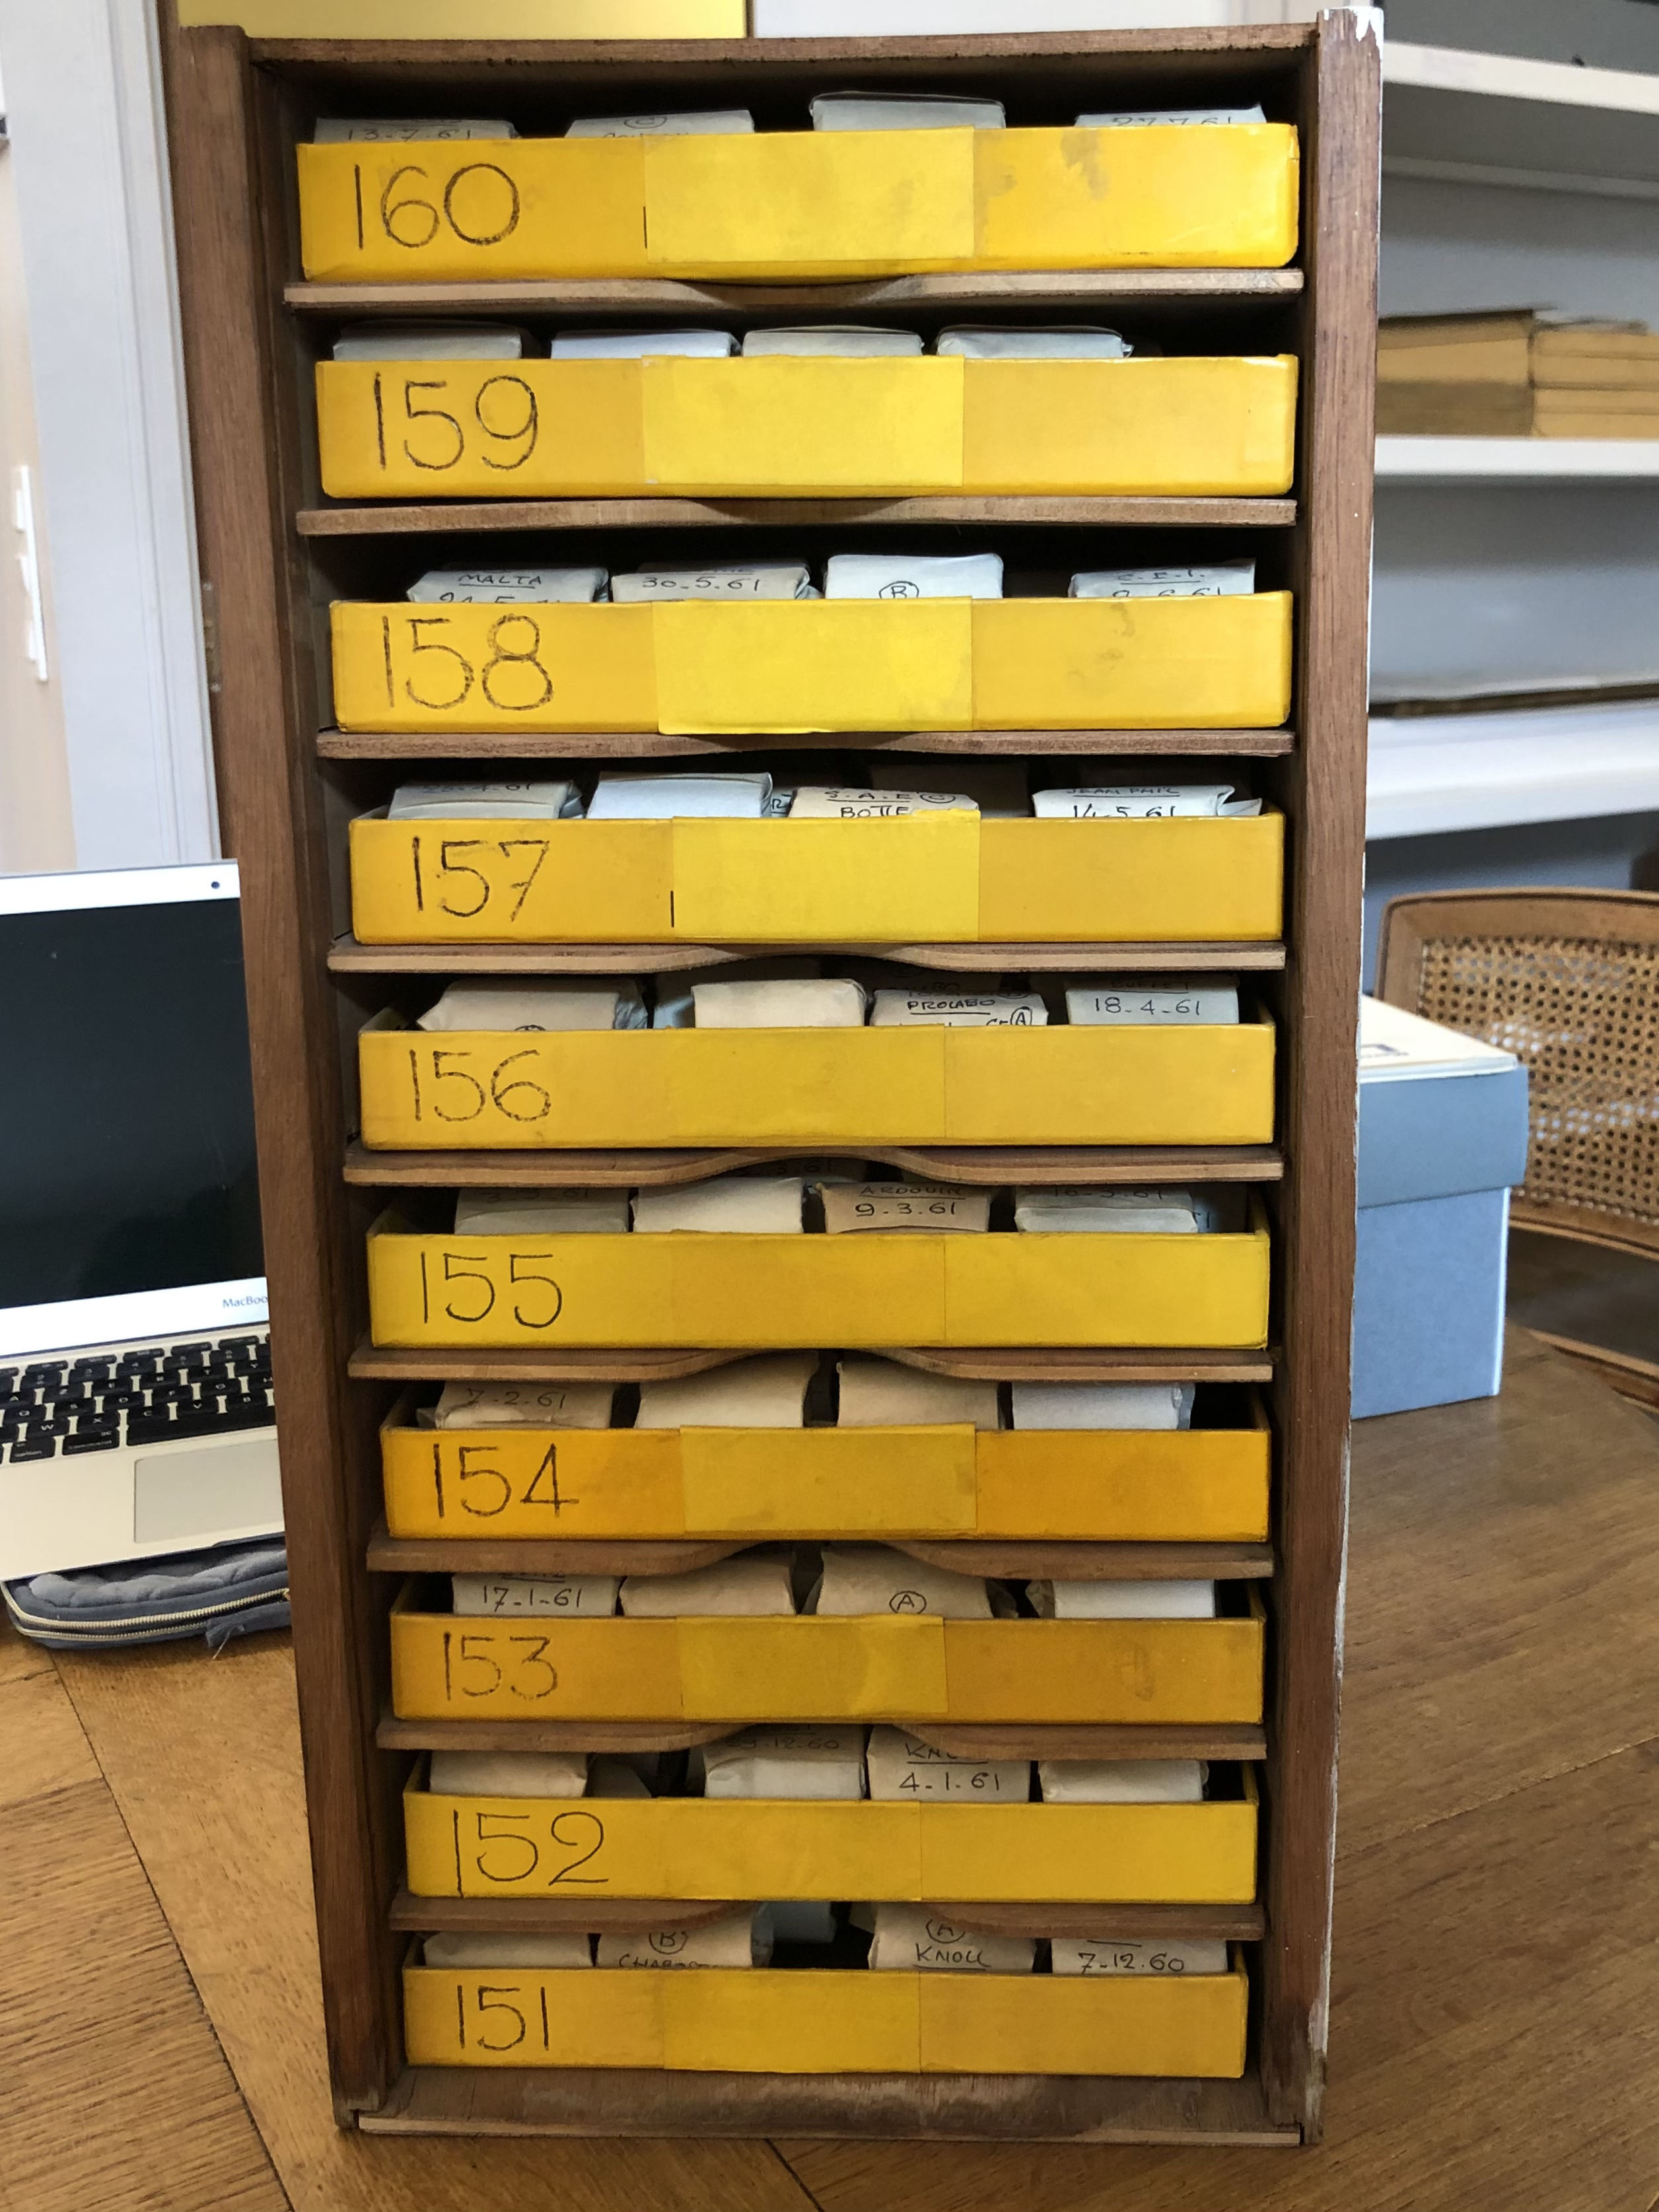
\includegraphics[width=0.75\linewidth]{Illustrations/tiroirs.jpg}
    \caption{Photo des tiroirs de pellicules numérisées}
    \label{fig:tiroirs}
\end{figure}

\begin{figure}[H]
    \centering
    \begin{subfigure}{0.24\textwidth}
        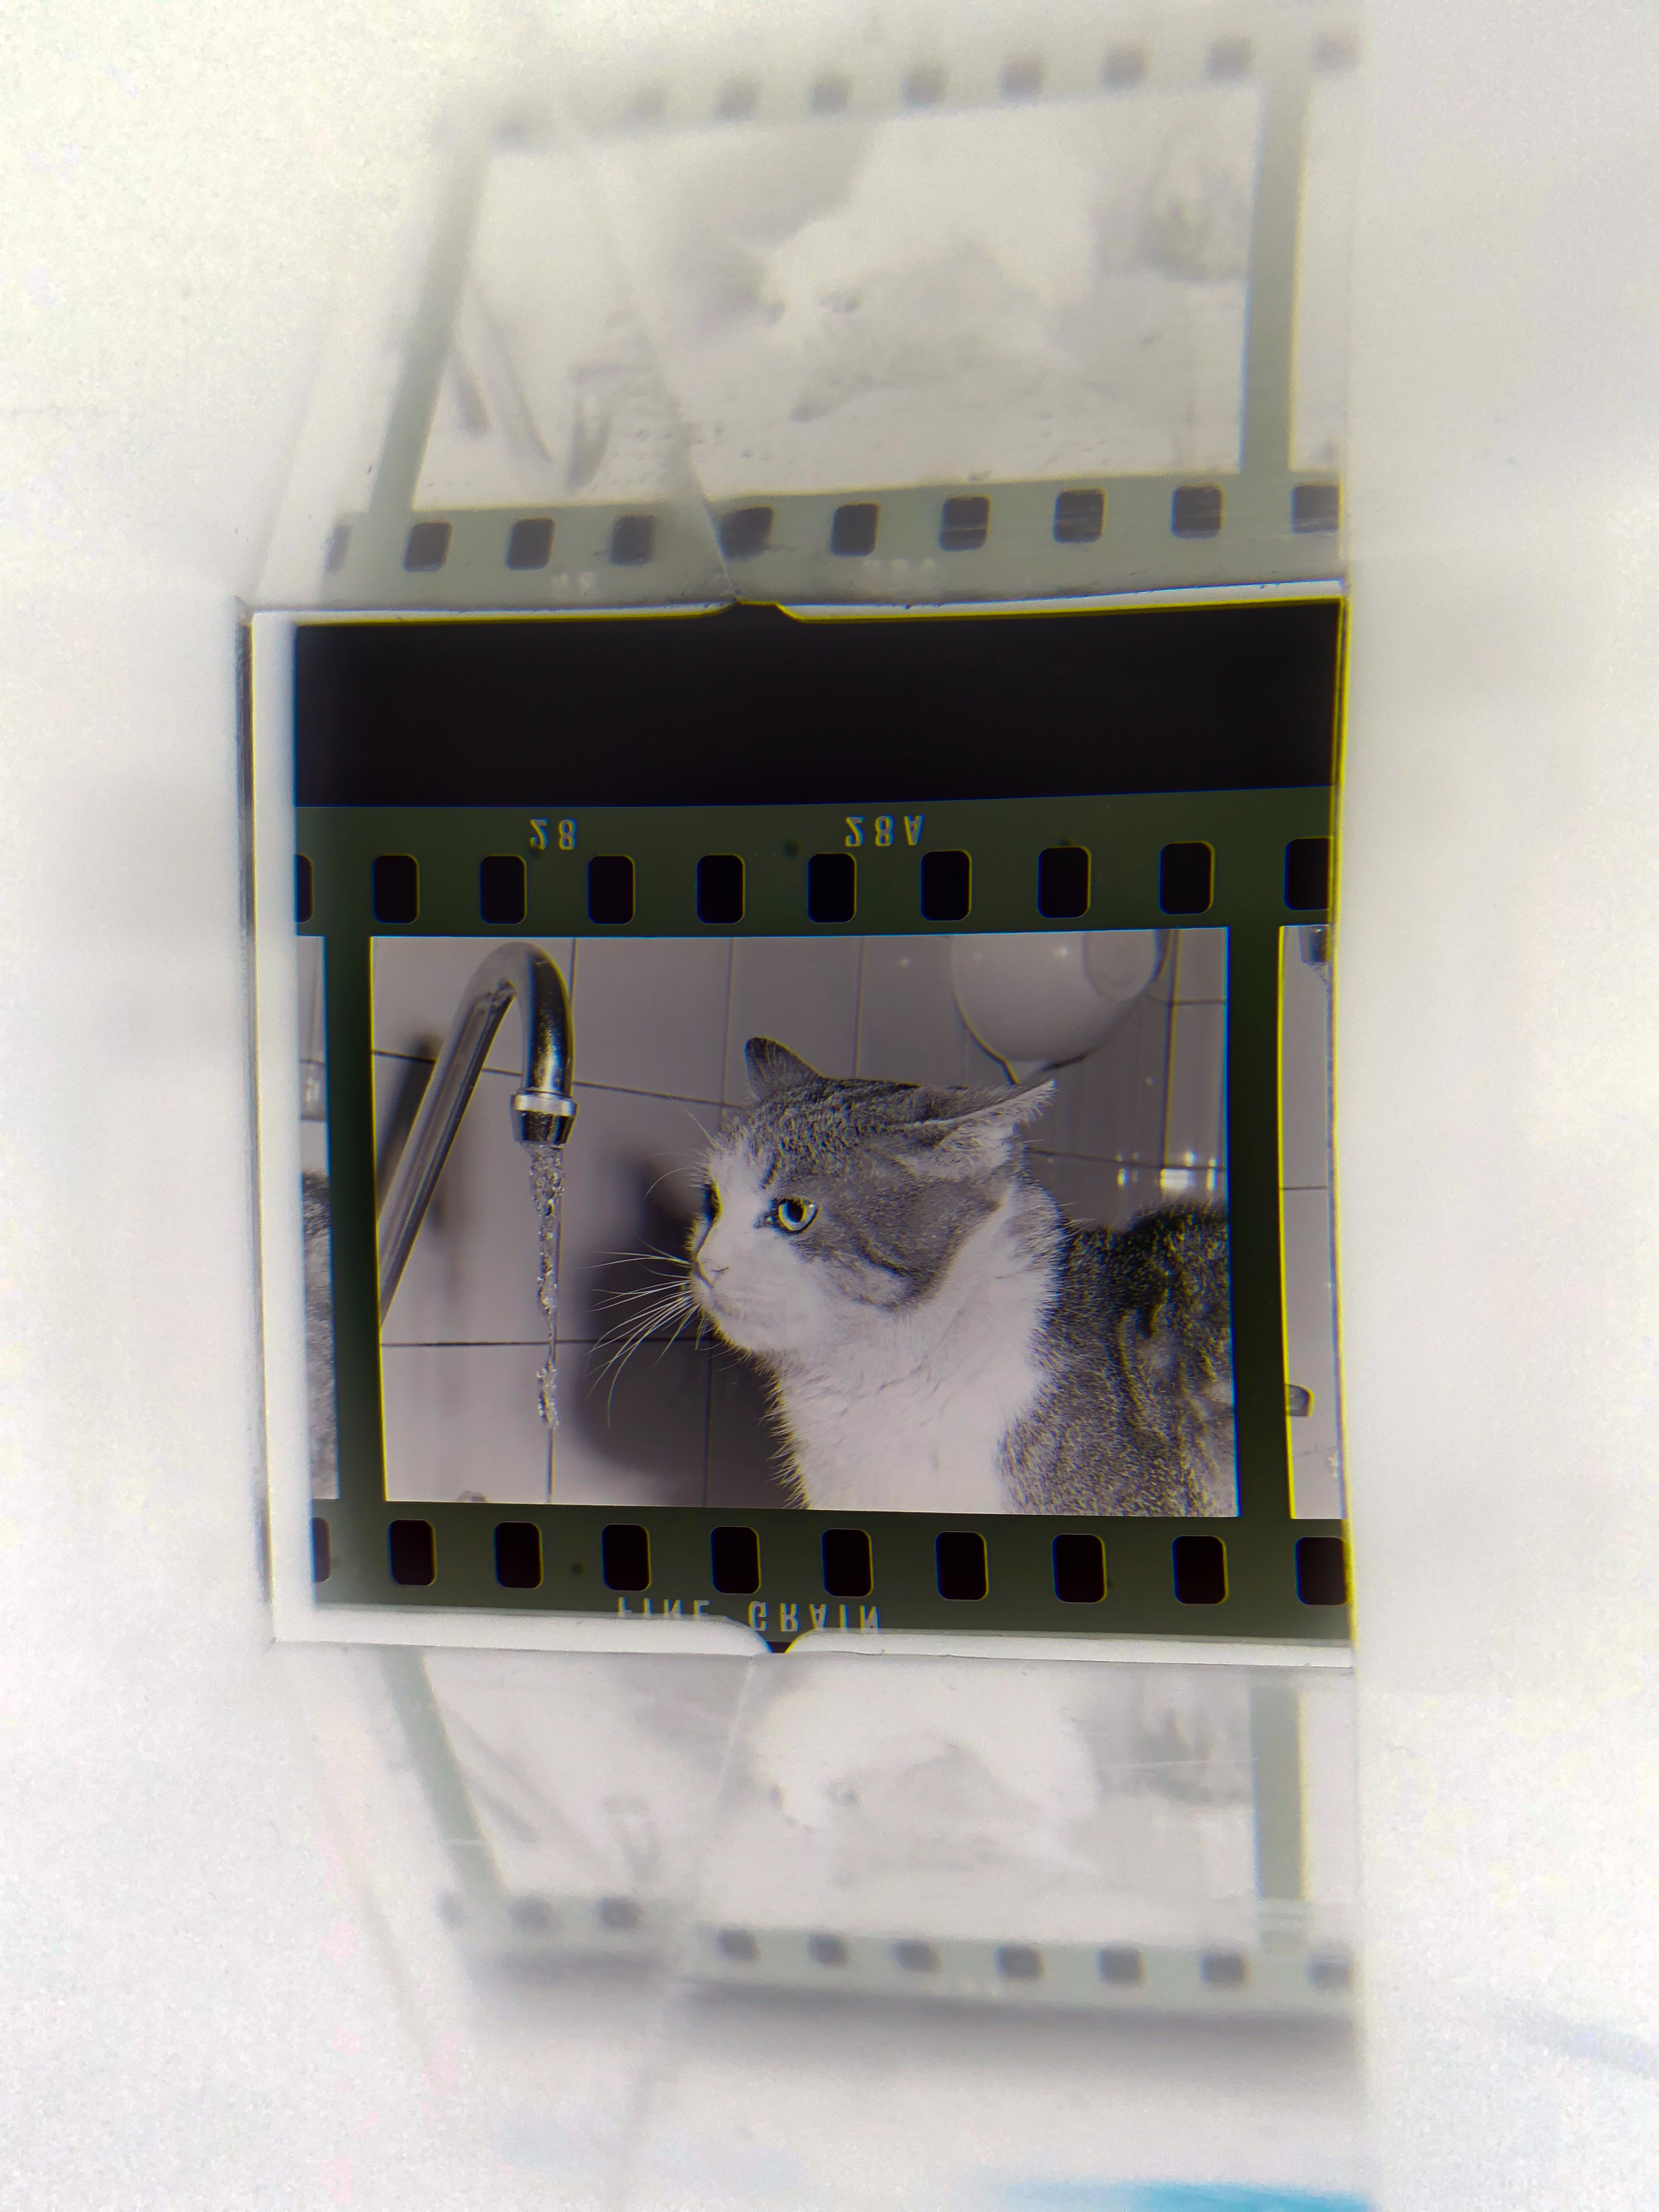
\includegraphics[width=\linewidth]{Illustrations/P1.jpg}
        \caption{}
    \end{subfigure}
    \begin{subfigure}{0.24\textwidth}
        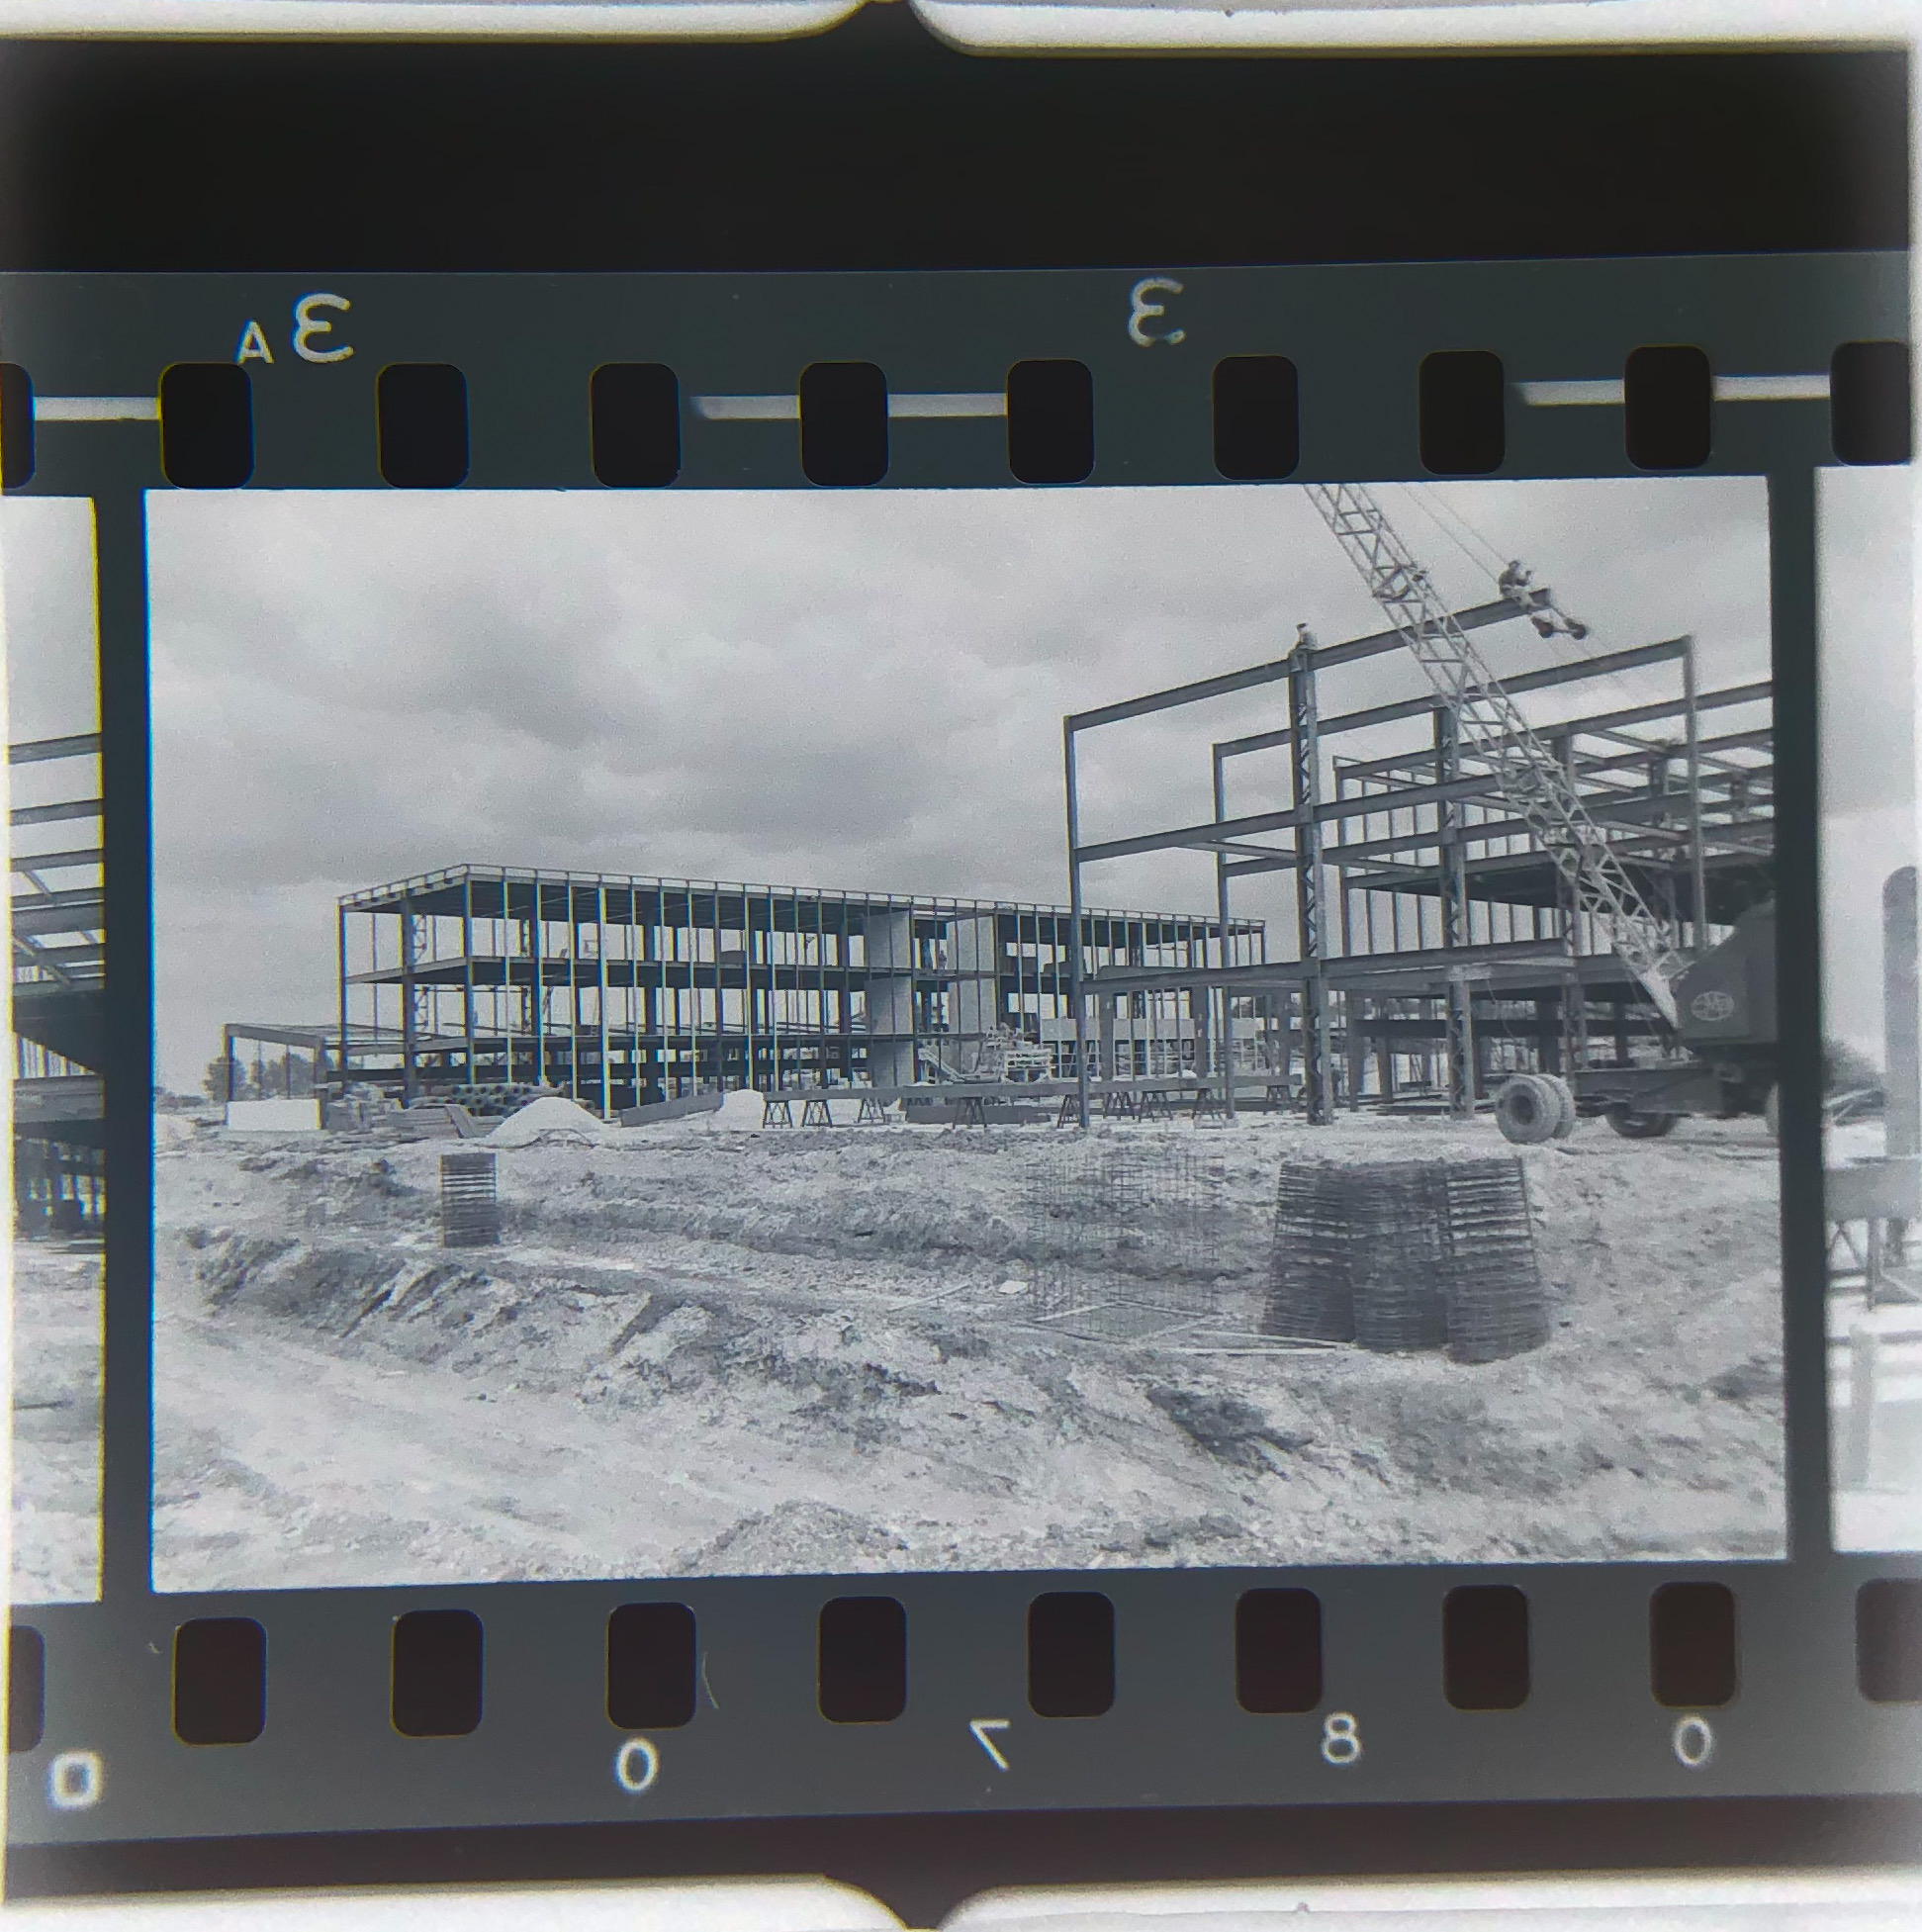
\includegraphics[width=\linewidth]{Illustrations/P2.jpg}
        \caption{}
    \end{subfigure}
    \begin{subfigure}{0.24\textwidth}
        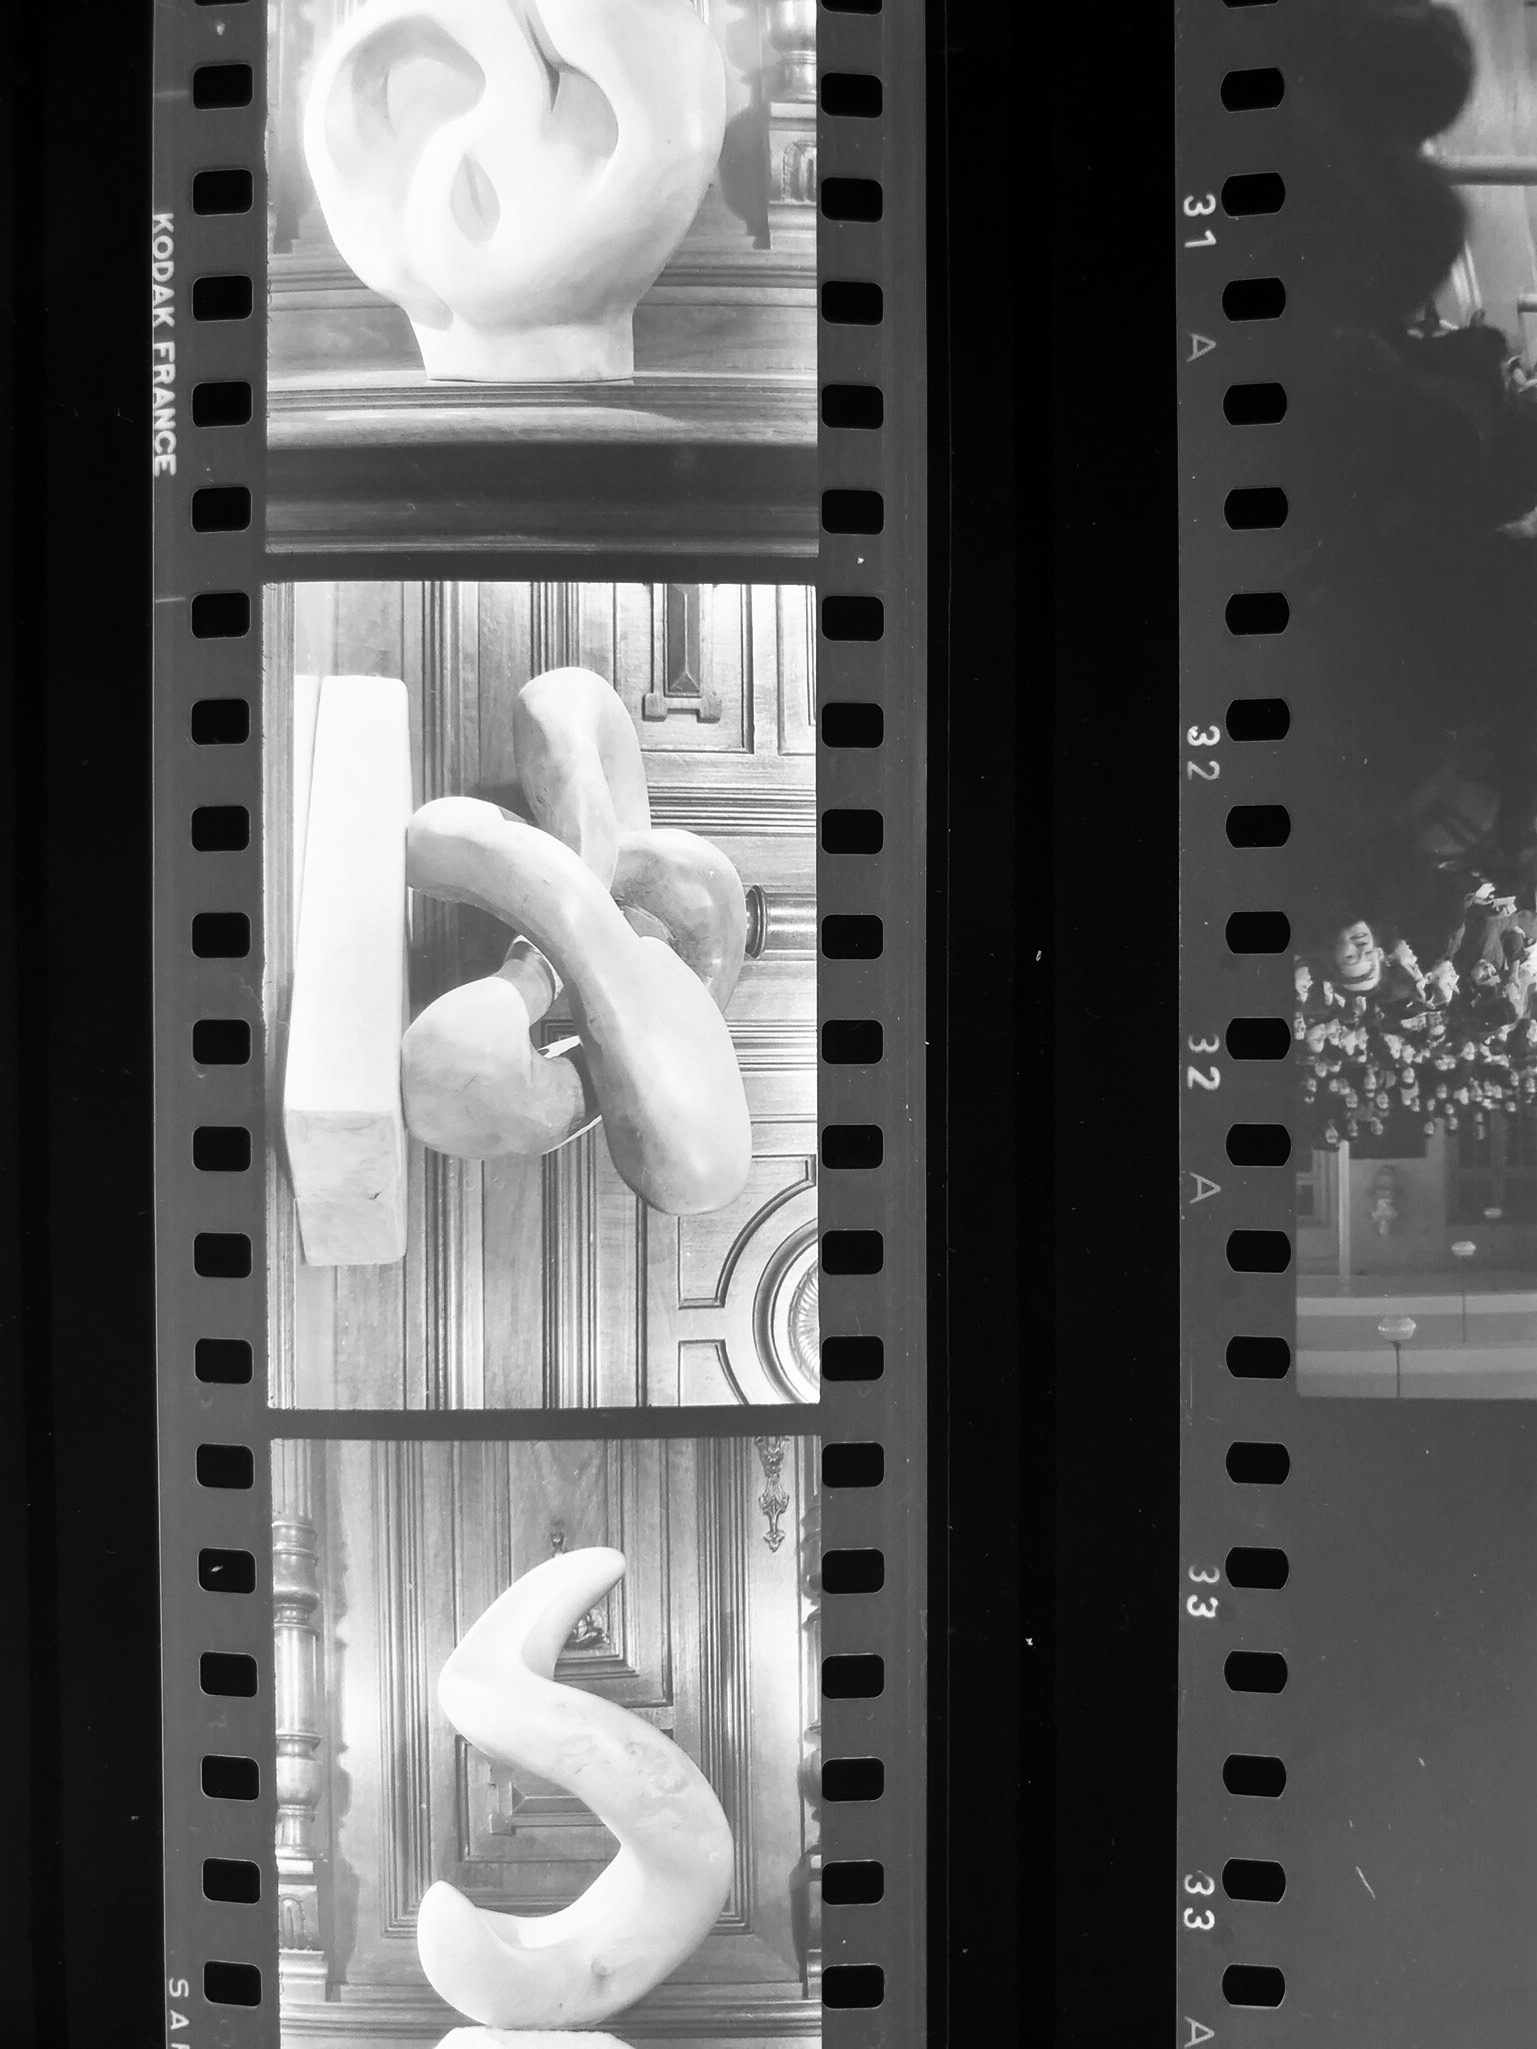
\includegraphics[width=\linewidth]{Illustrations/P3.jpg}
        \caption{}
    \end{subfigure}
    \begin{subfigure}{0.24\textwidth}
        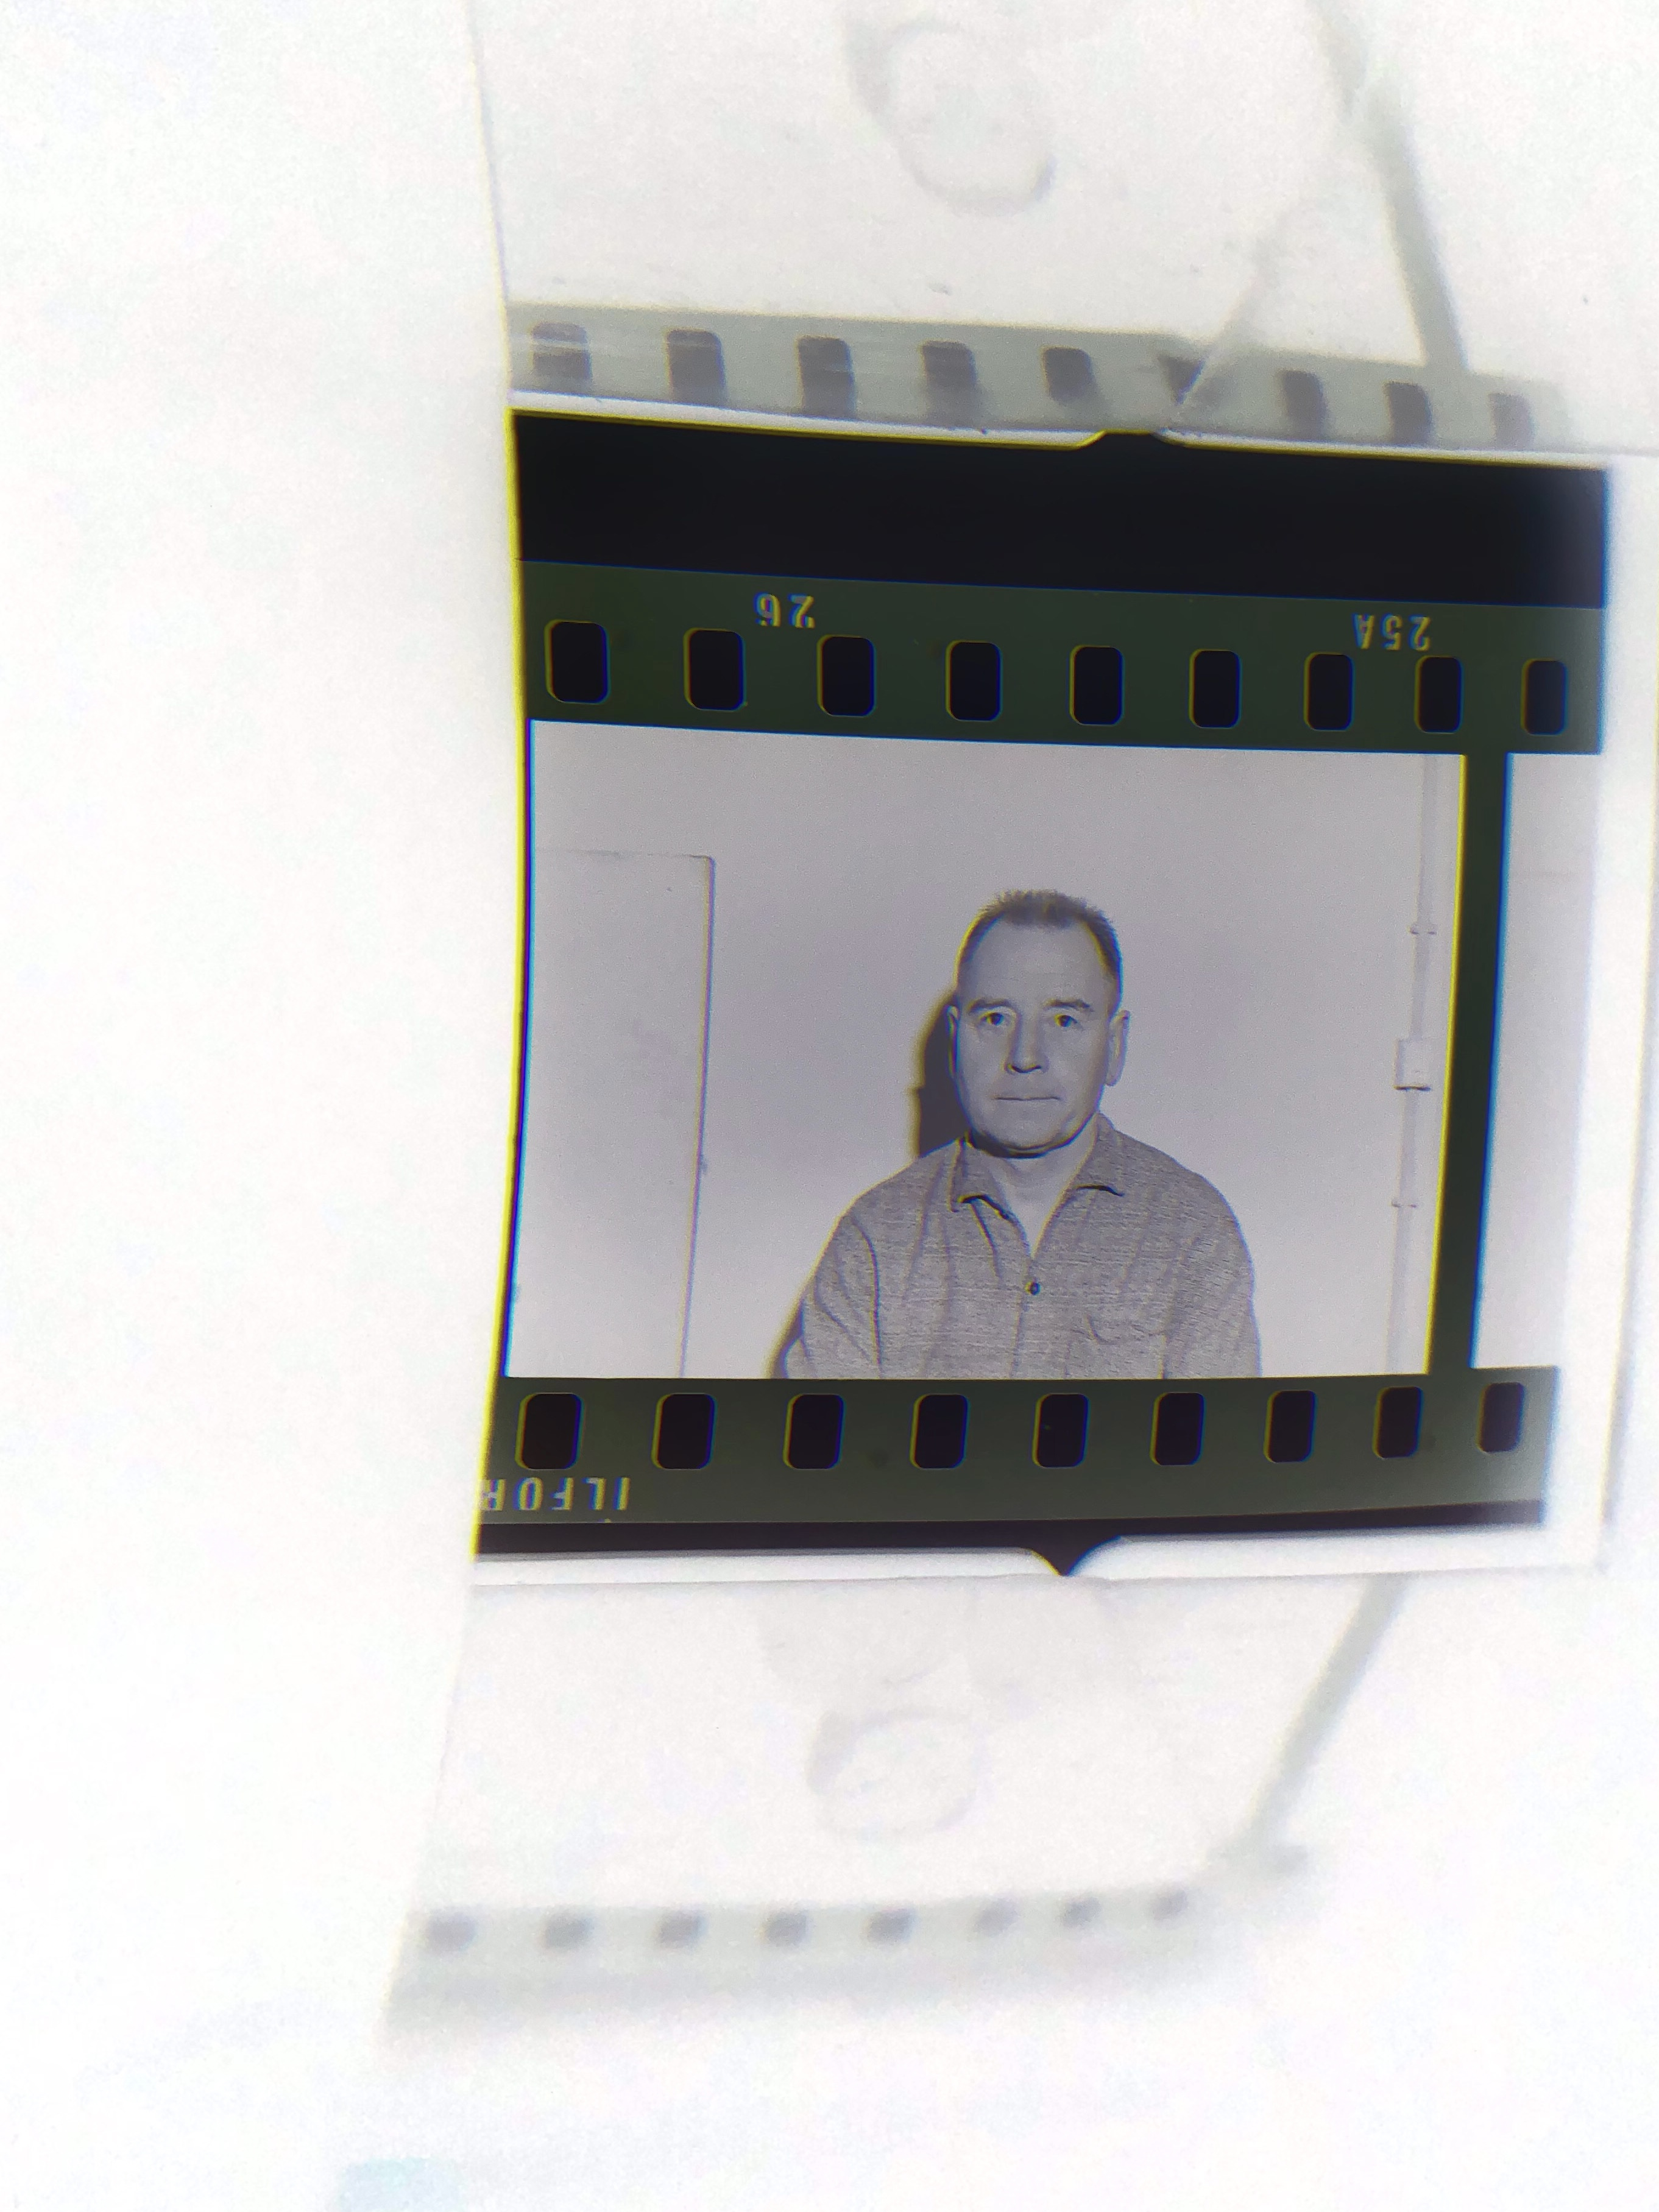
\includegraphics[width=\linewidth]{Illustrations/P4.jpg}
        \caption{}
    \end{subfigure}
    \begin{subfigure}{0.20\textwidth}
        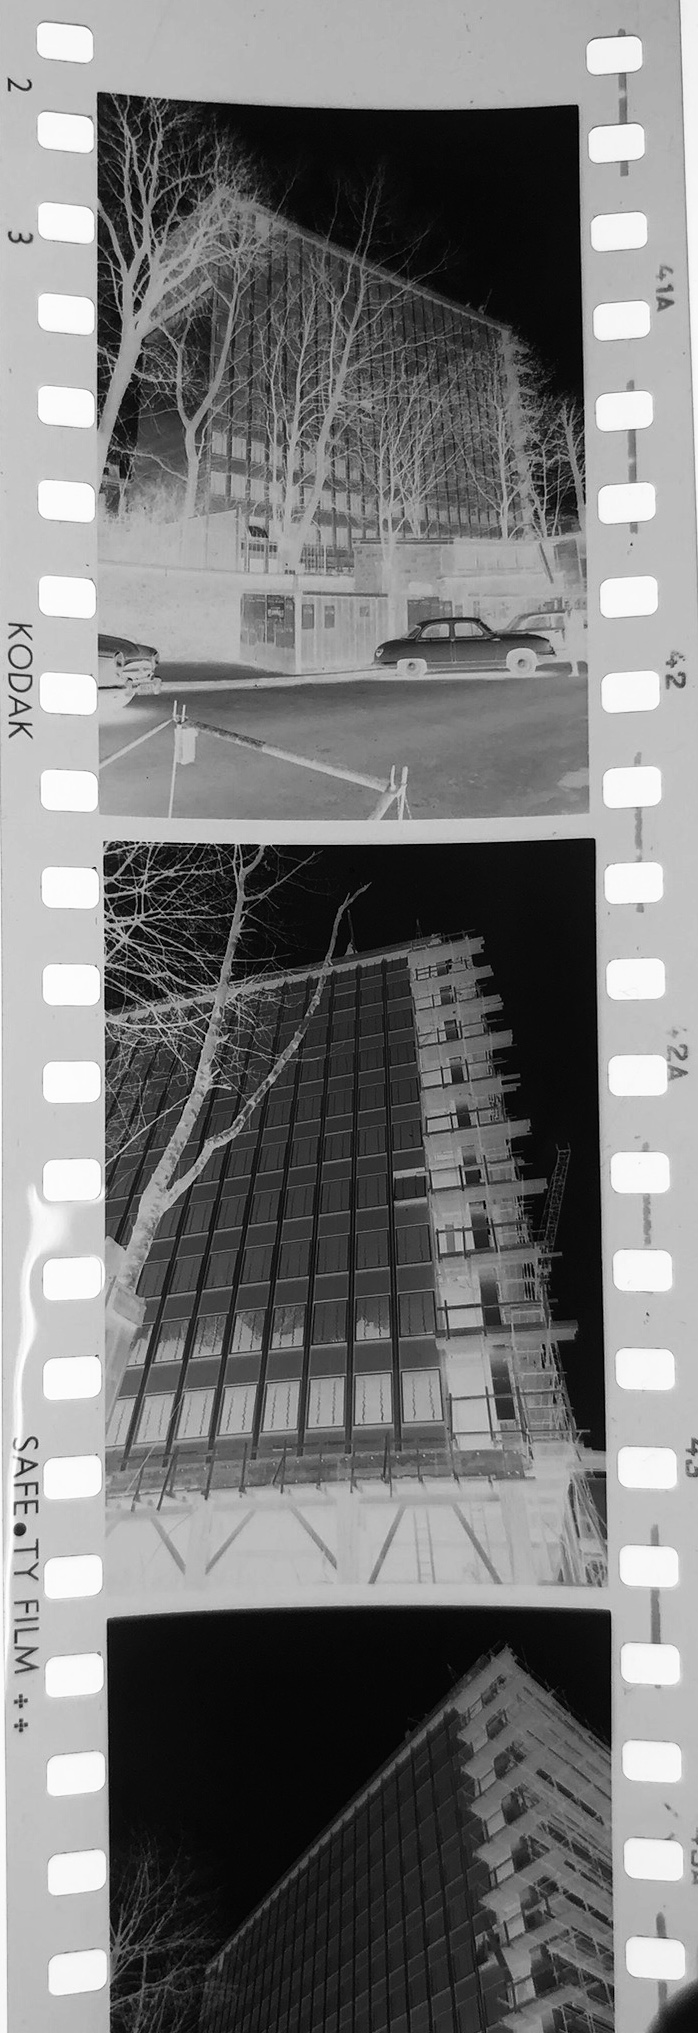
\includegraphics[width=\linewidth]{Illustrations/P5.jpg}
        \caption{}
    \end{subfigure}
    \begin{subfigure}{0.24\textwidth}
        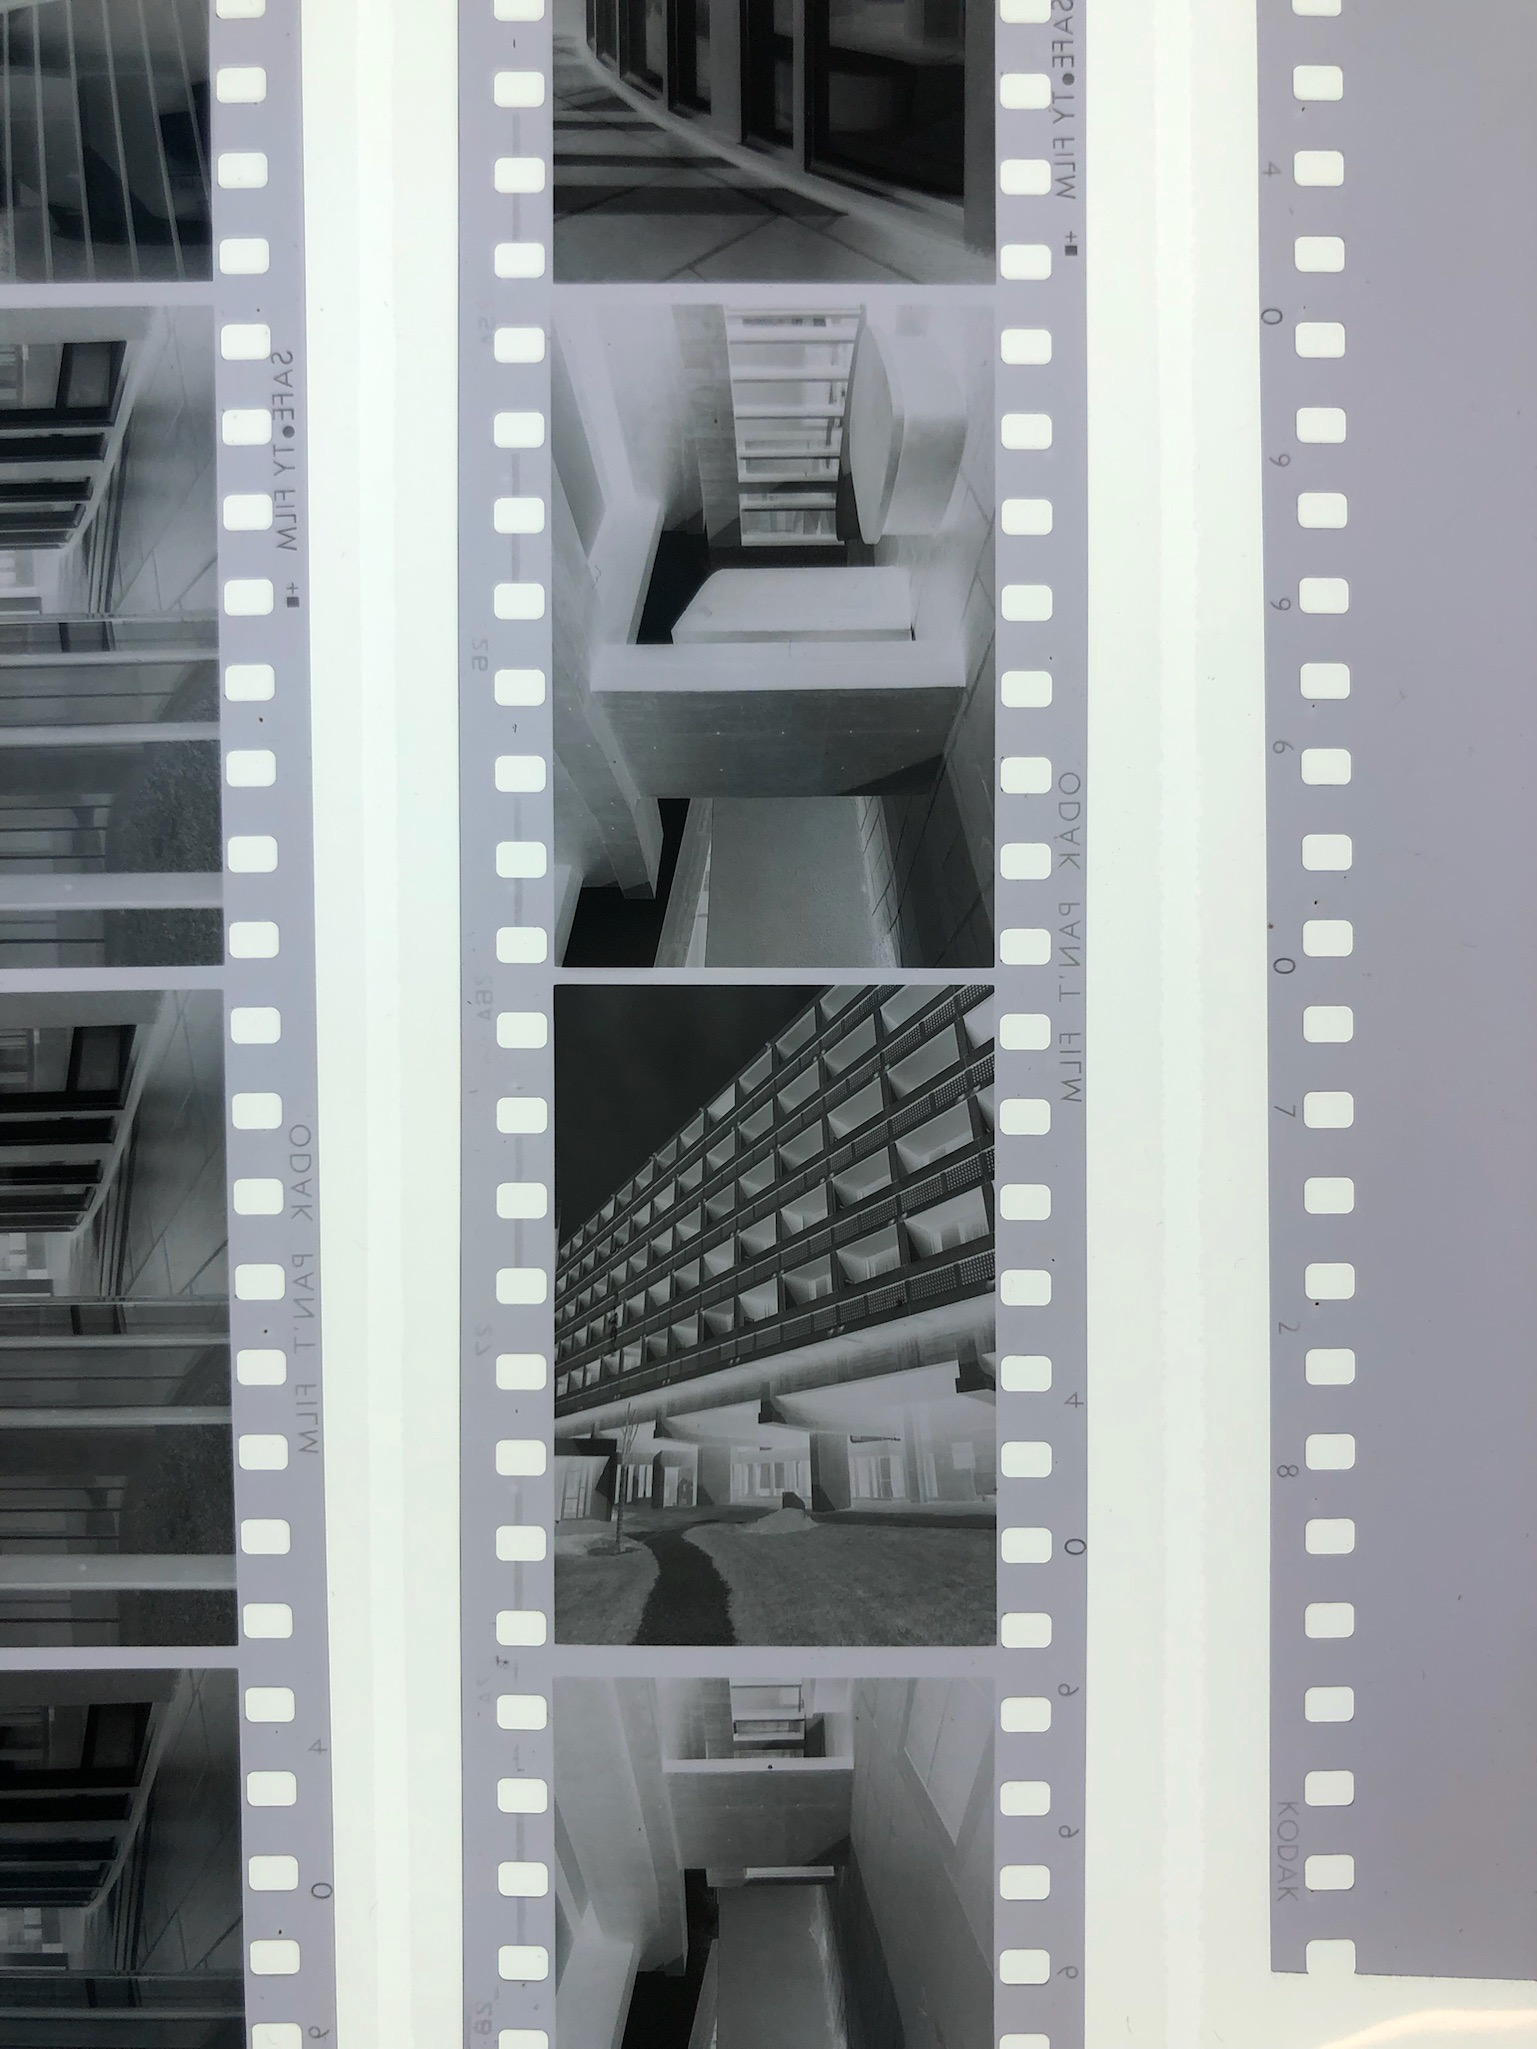
\includegraphics[width=\linewidth]{Illustrations/P6.jpg}
        \caption{}
    \end{subfigure}
    \begin{subfigure}{0.24\textwidth}
        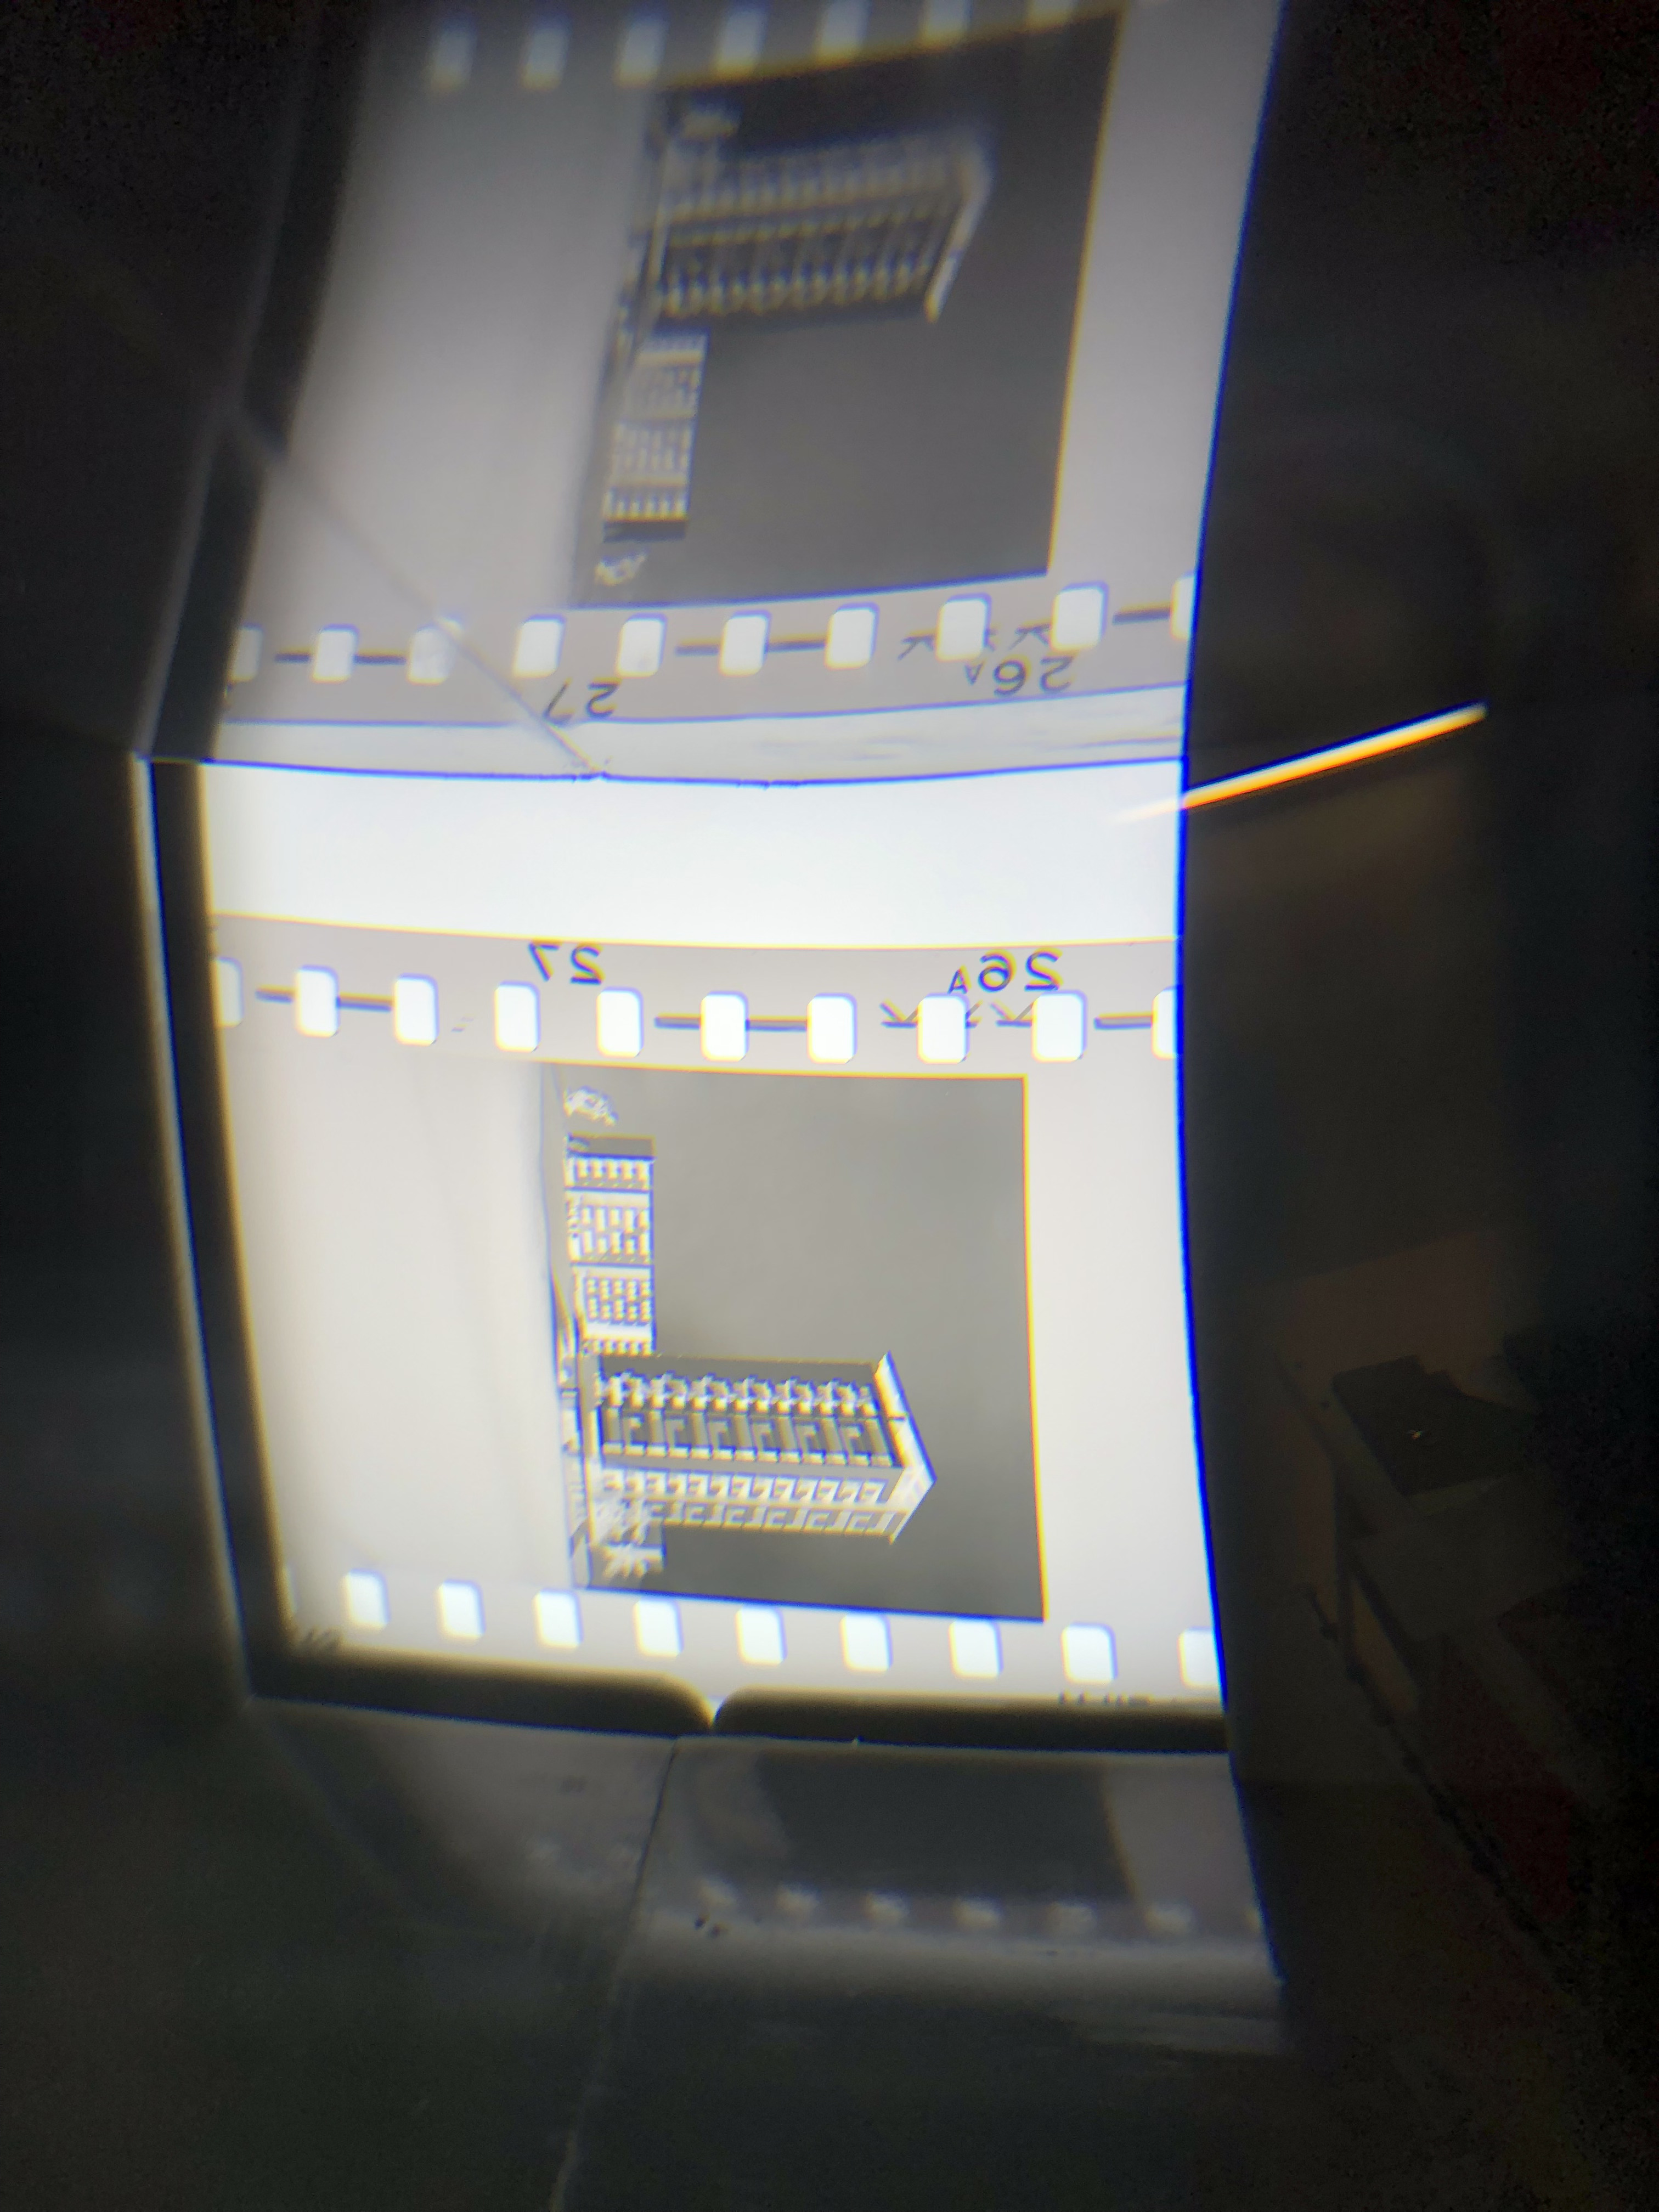
\includegraphics[width=\linewidth]{Illustrations/P7.jpg}
        \caption{}
    \end{subfigure}
    \begin{subfigure}{0.24\textwidth}
        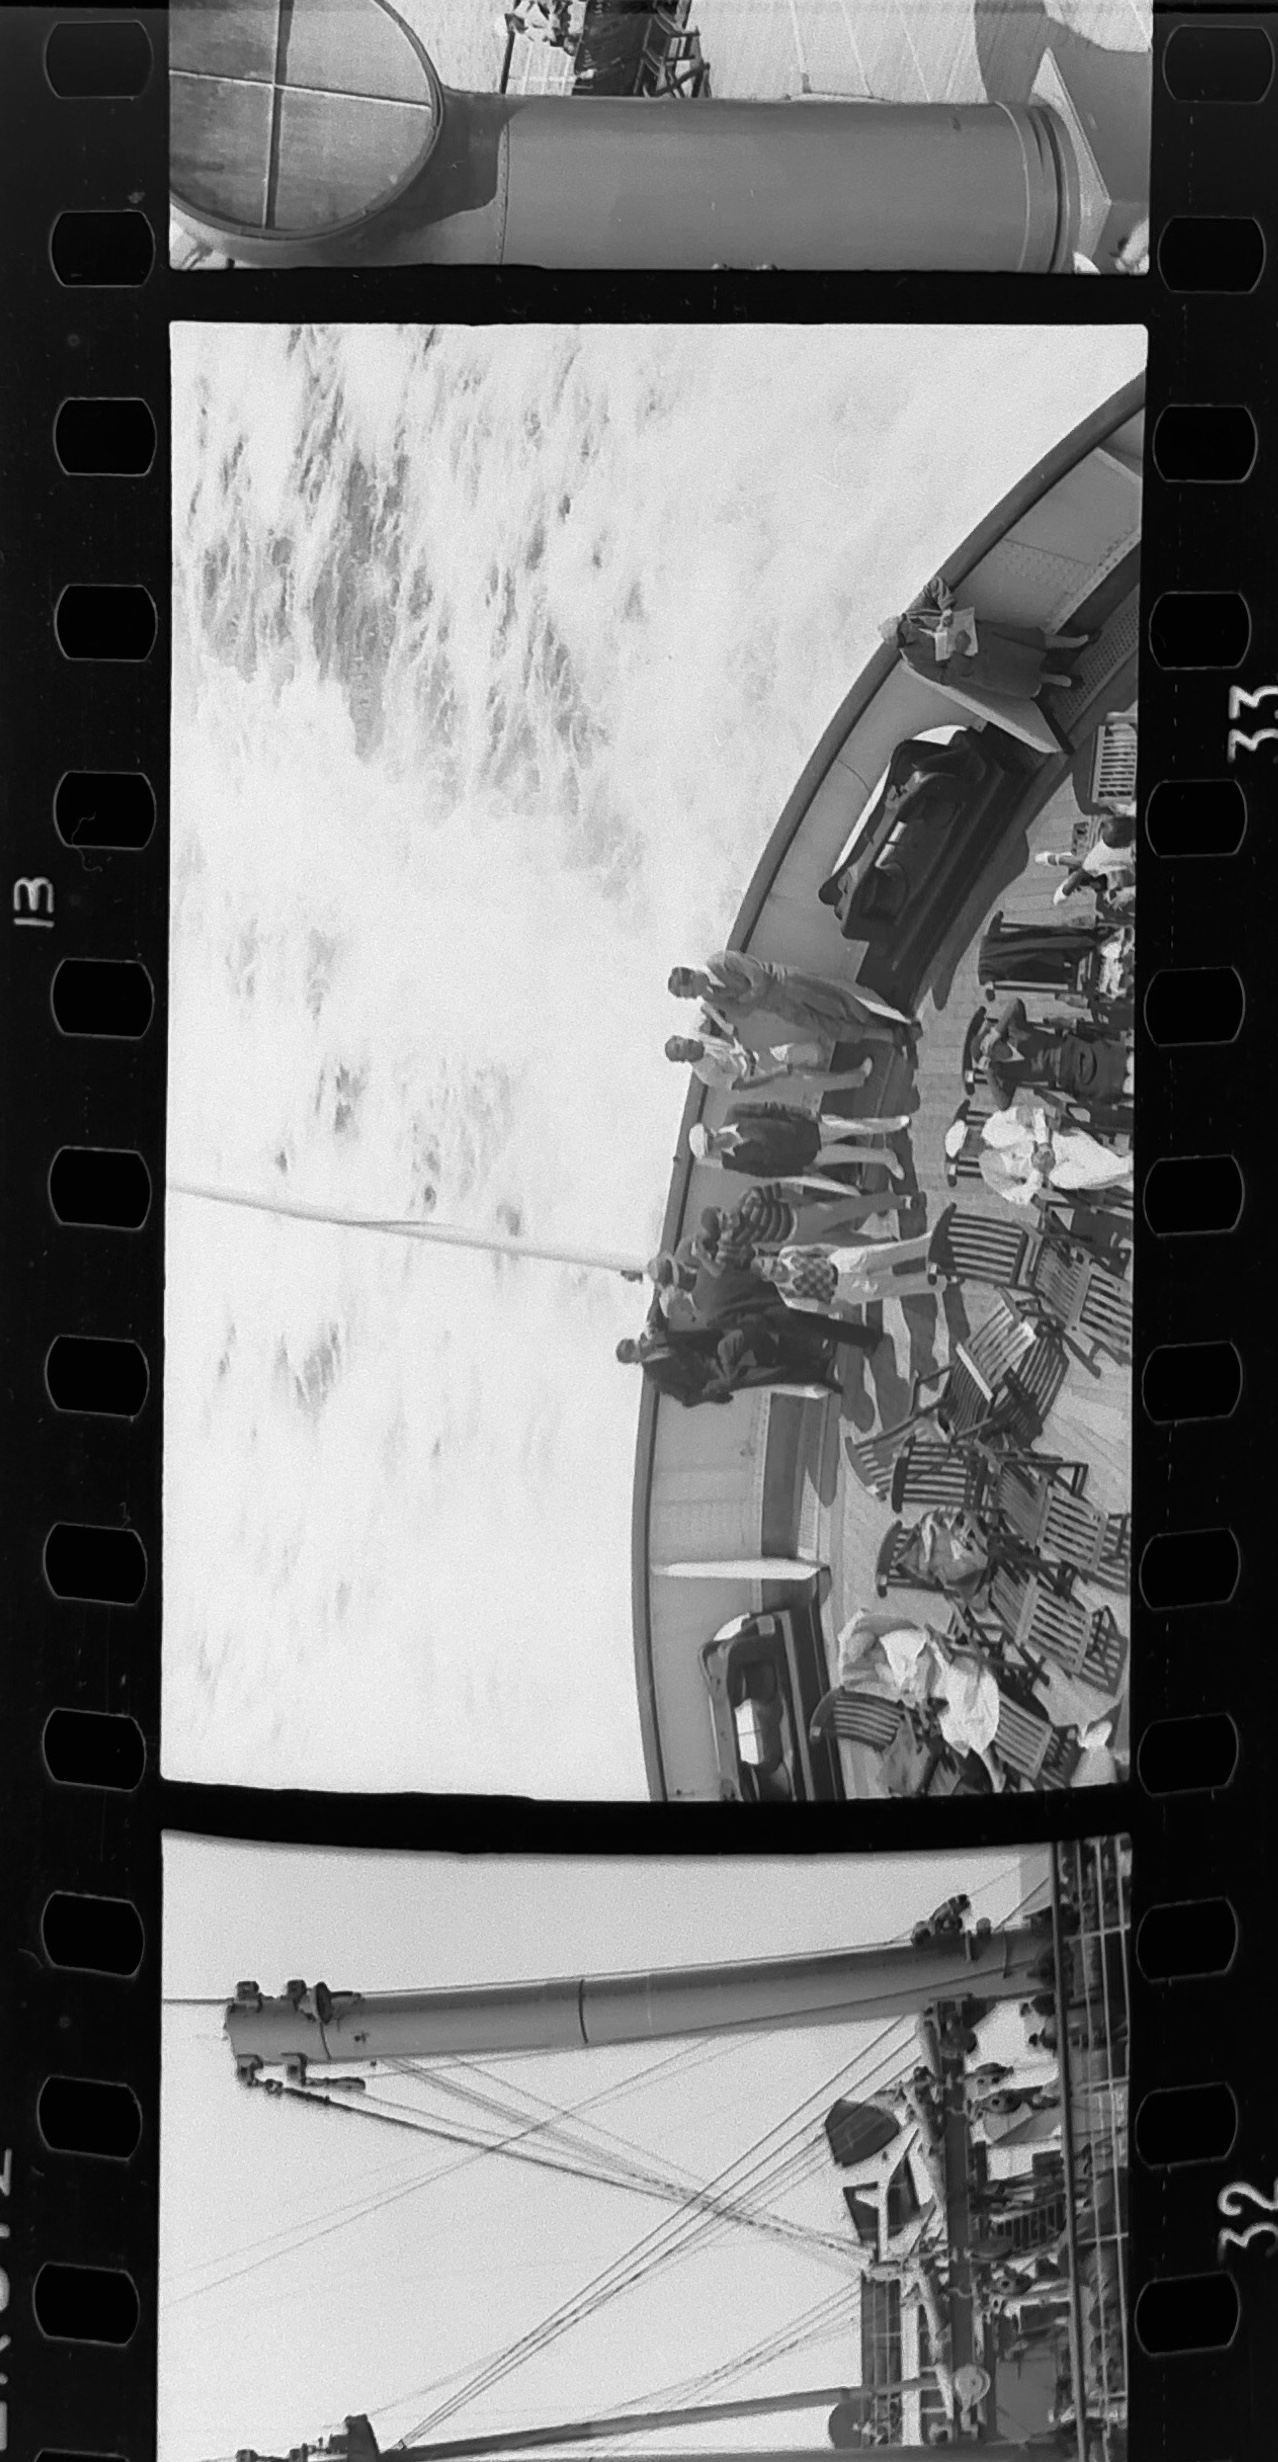
\includegraphics[width=\linewidth]{Illustrations/P8.jpg}
        \caption{}
    \end{subfigure}    \begin{subfigure}{0.24\textwidth}
        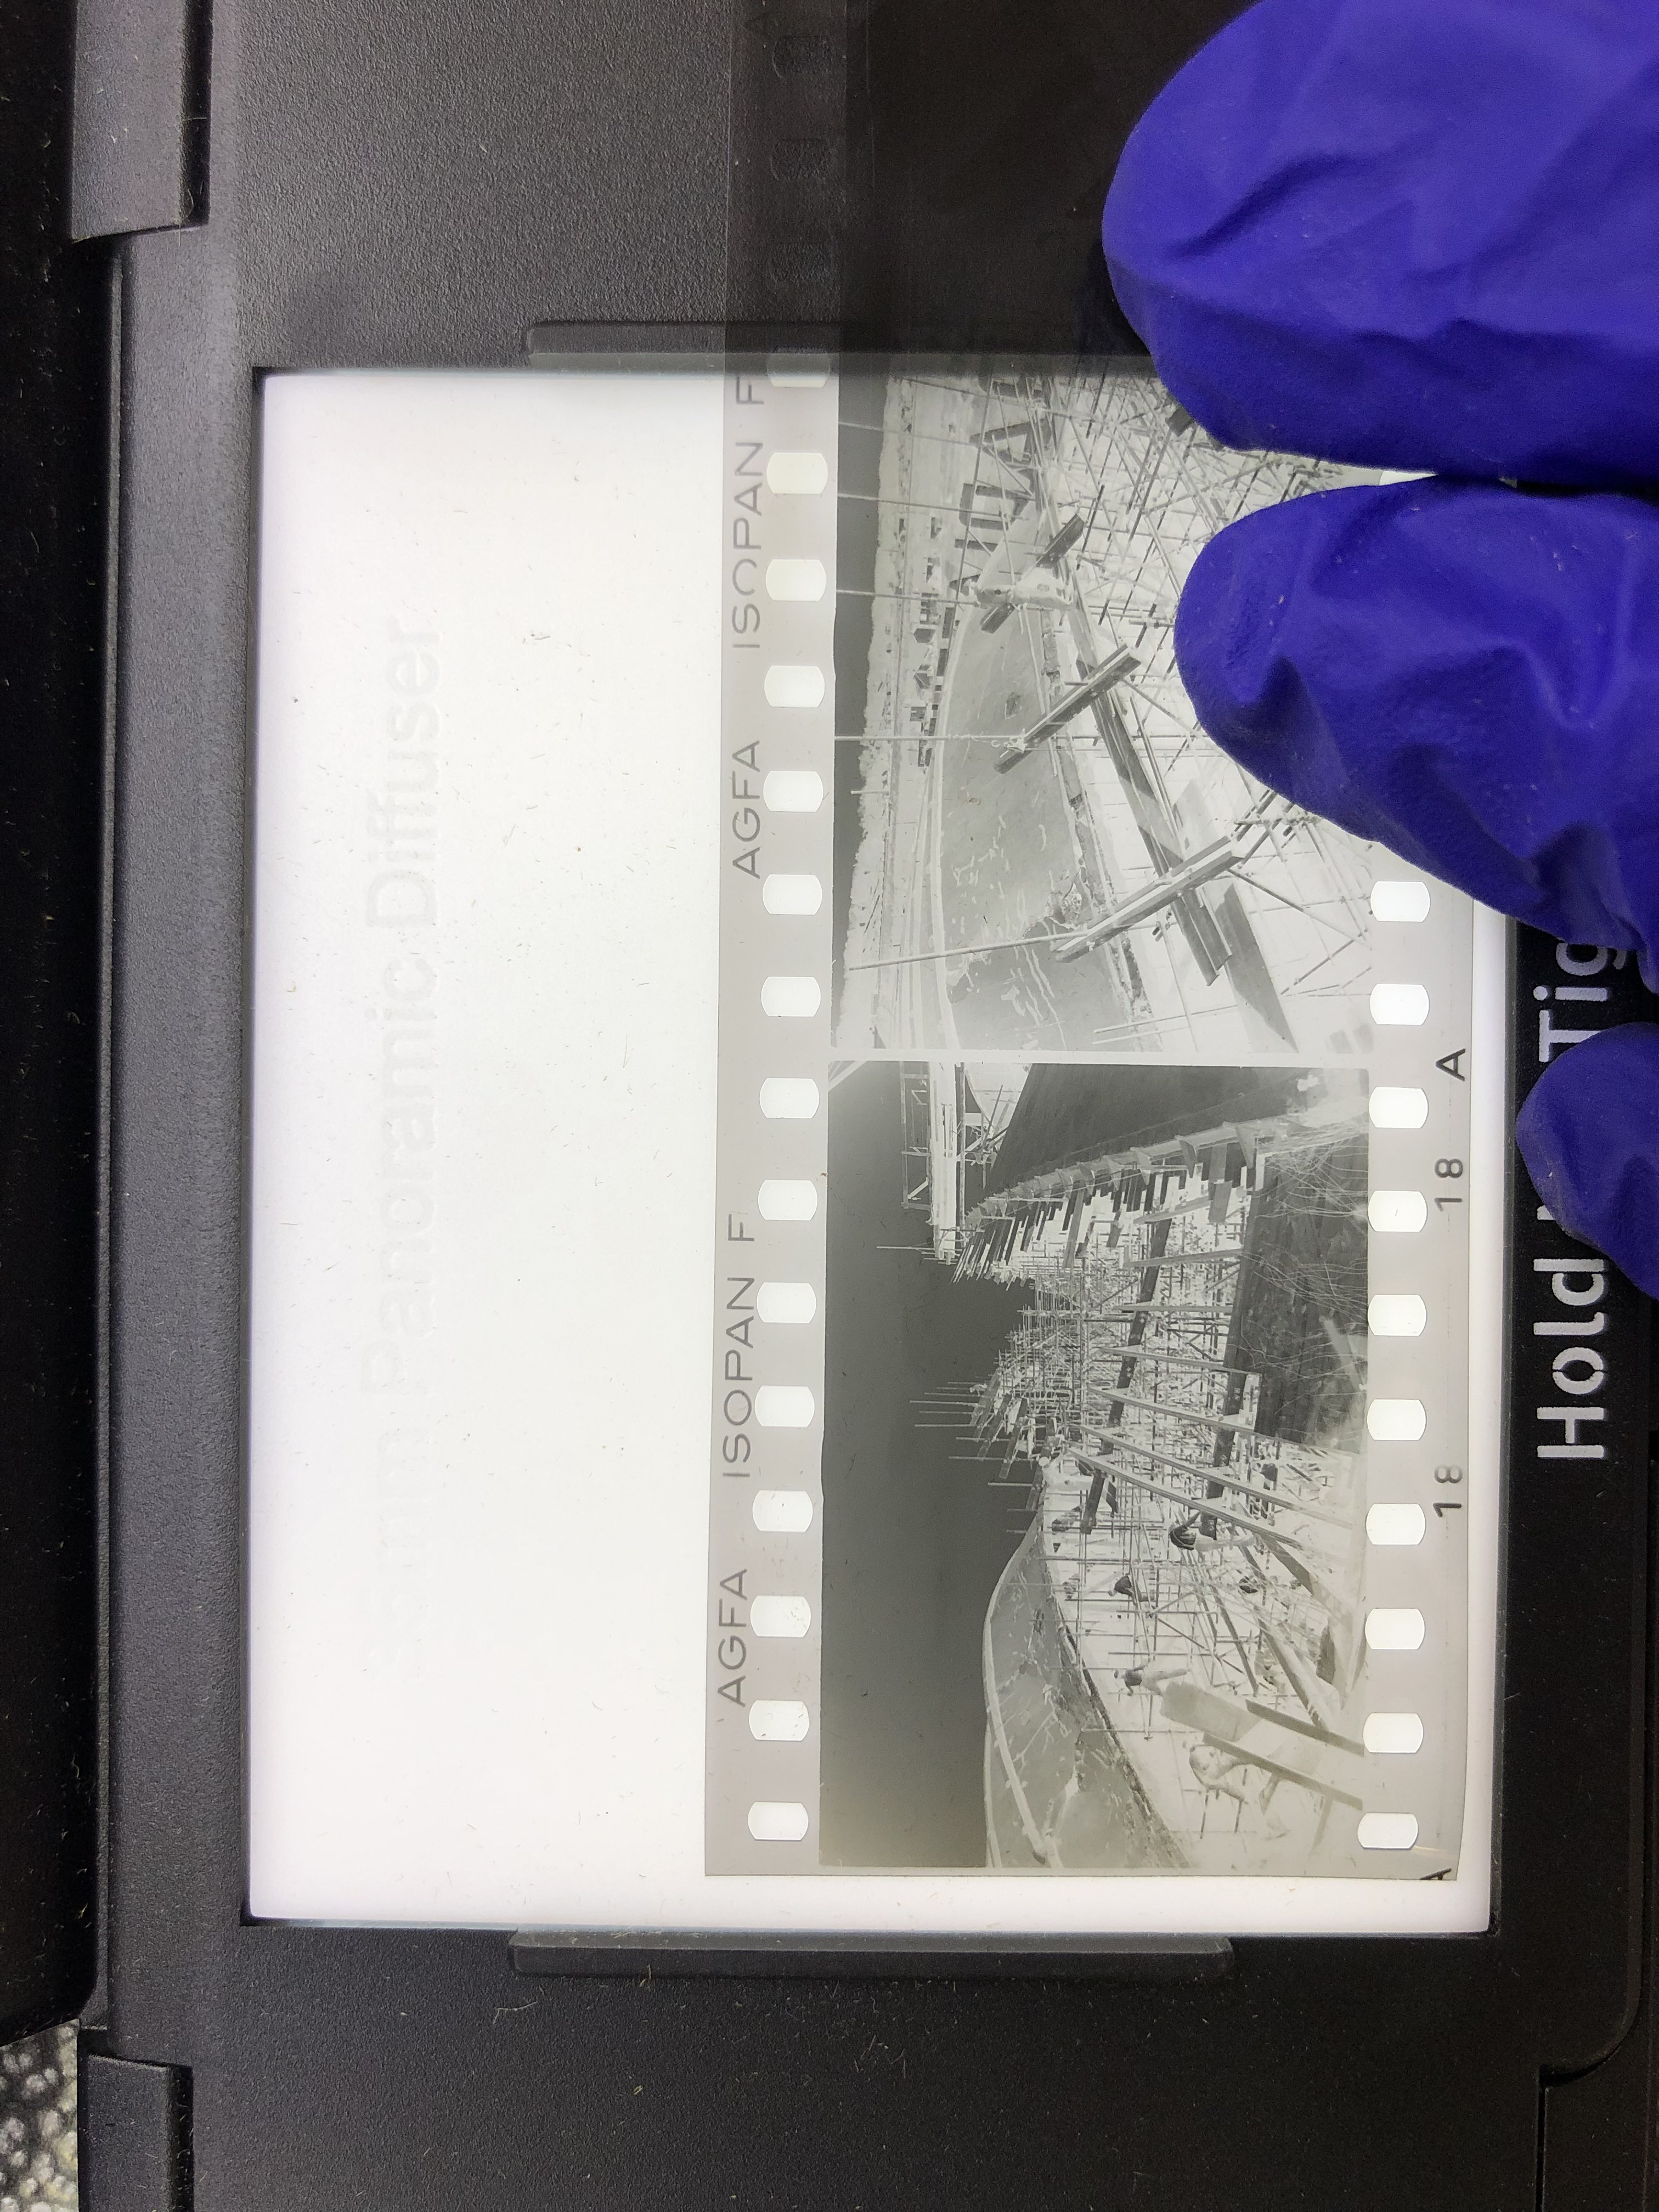
\includegraphics[width=\linewidth]{Illustrations/P9.jpg}
        \caption{}
    \end{subfigure}
    \begin{subfigure}{0.24\textwidth}
        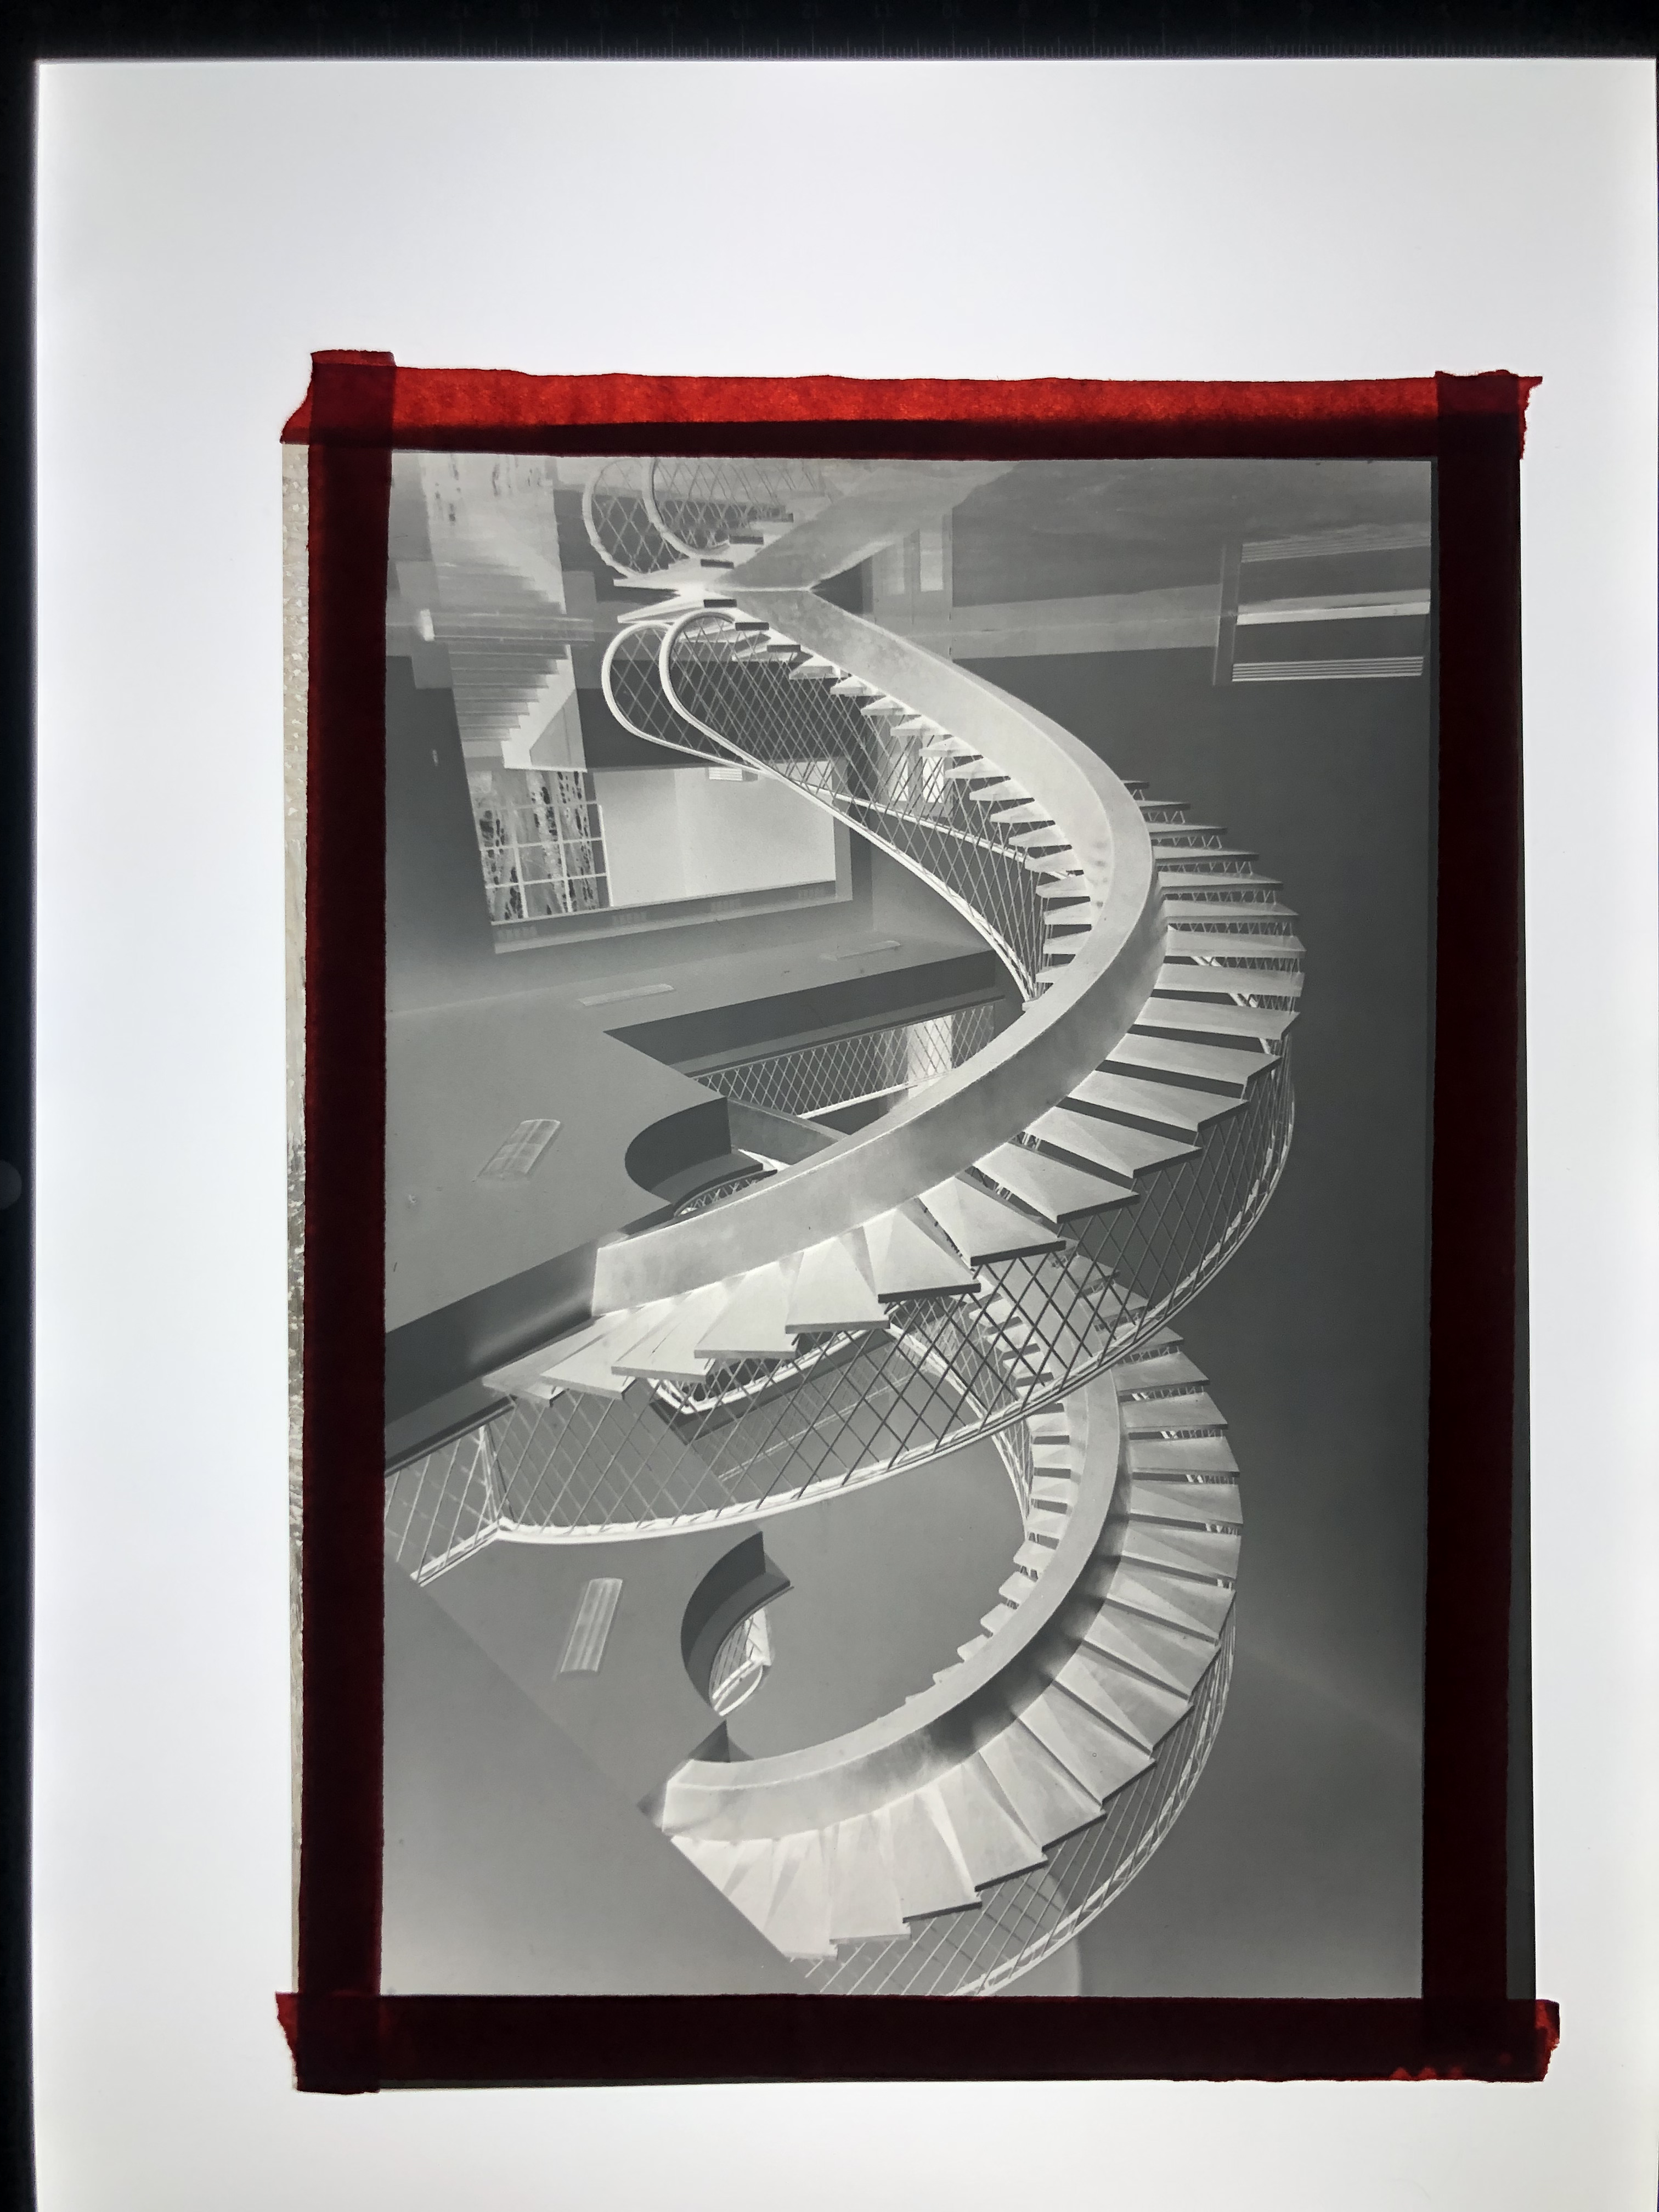
\includegraphics[width=\linewidth]{Illustrations/P10.jpg}
        \caption{}
    \end{subfigure}
    \begin{subfigure}{0.24\textwidth}
        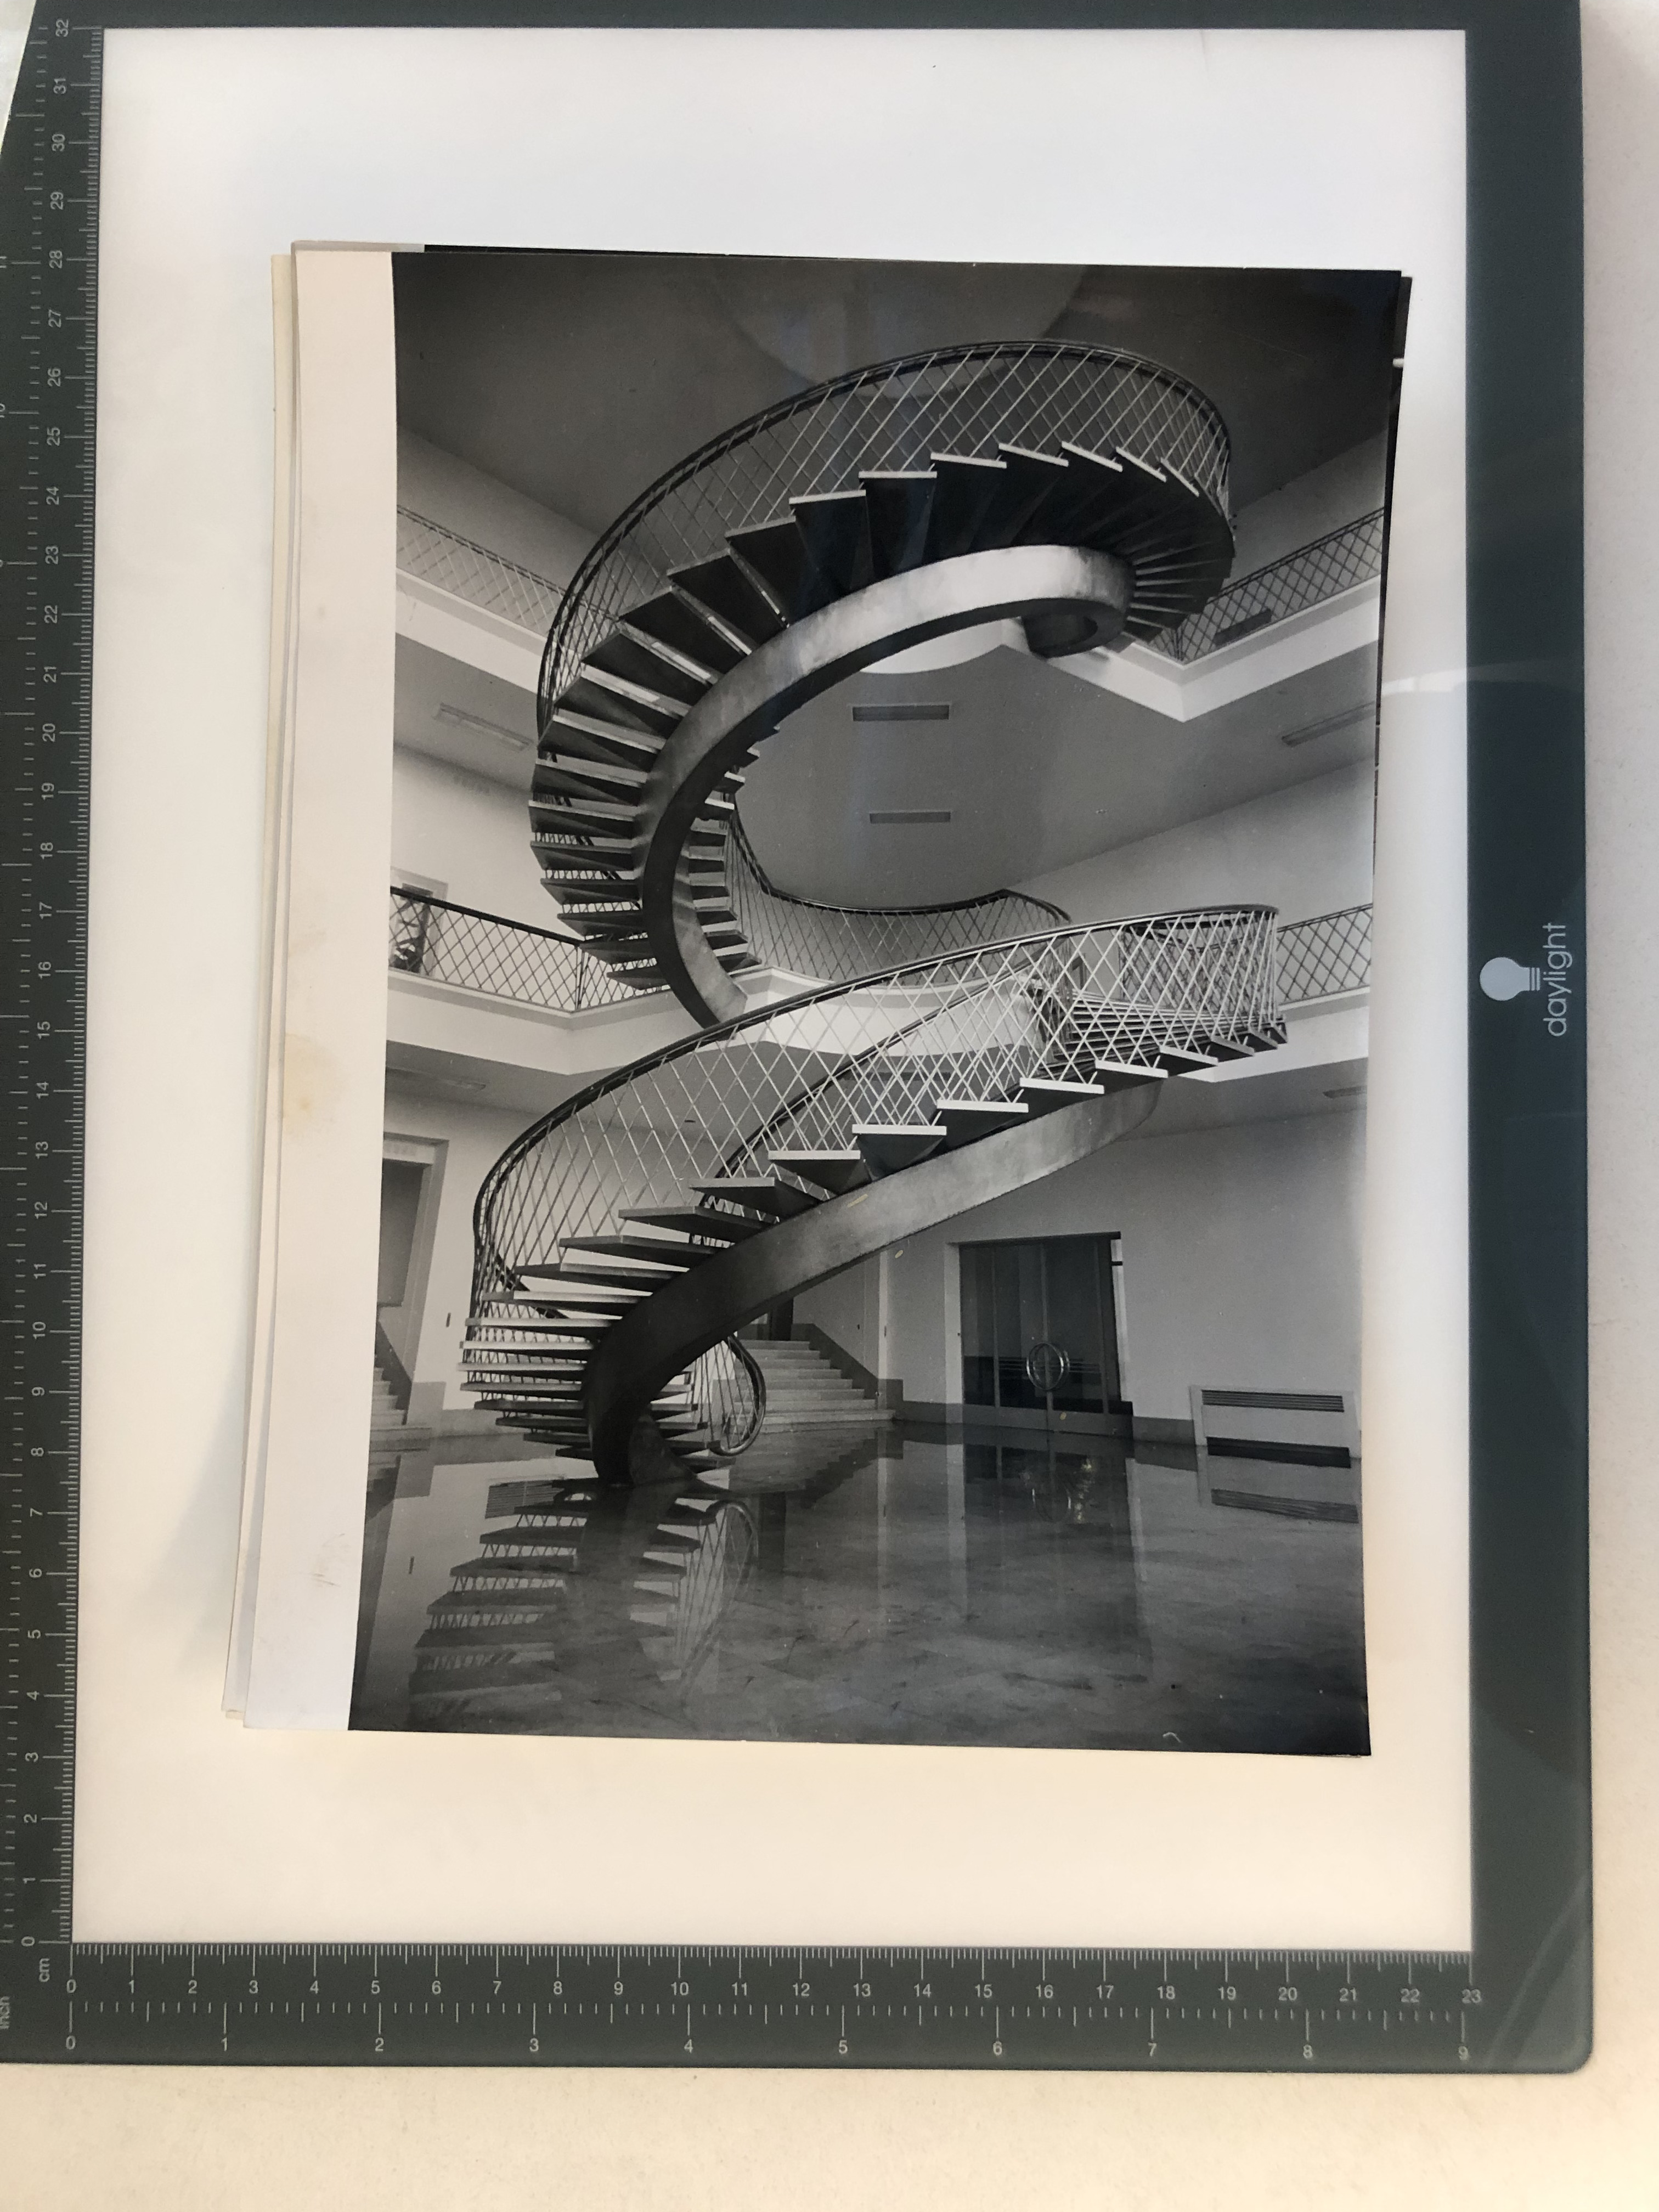
\includegraphics[width=\linewidth]{Illustrations/P11.jpg}
        \caption{}
    \end{subfigure}
    \begin{subfigure}{0.24\textwidth}
        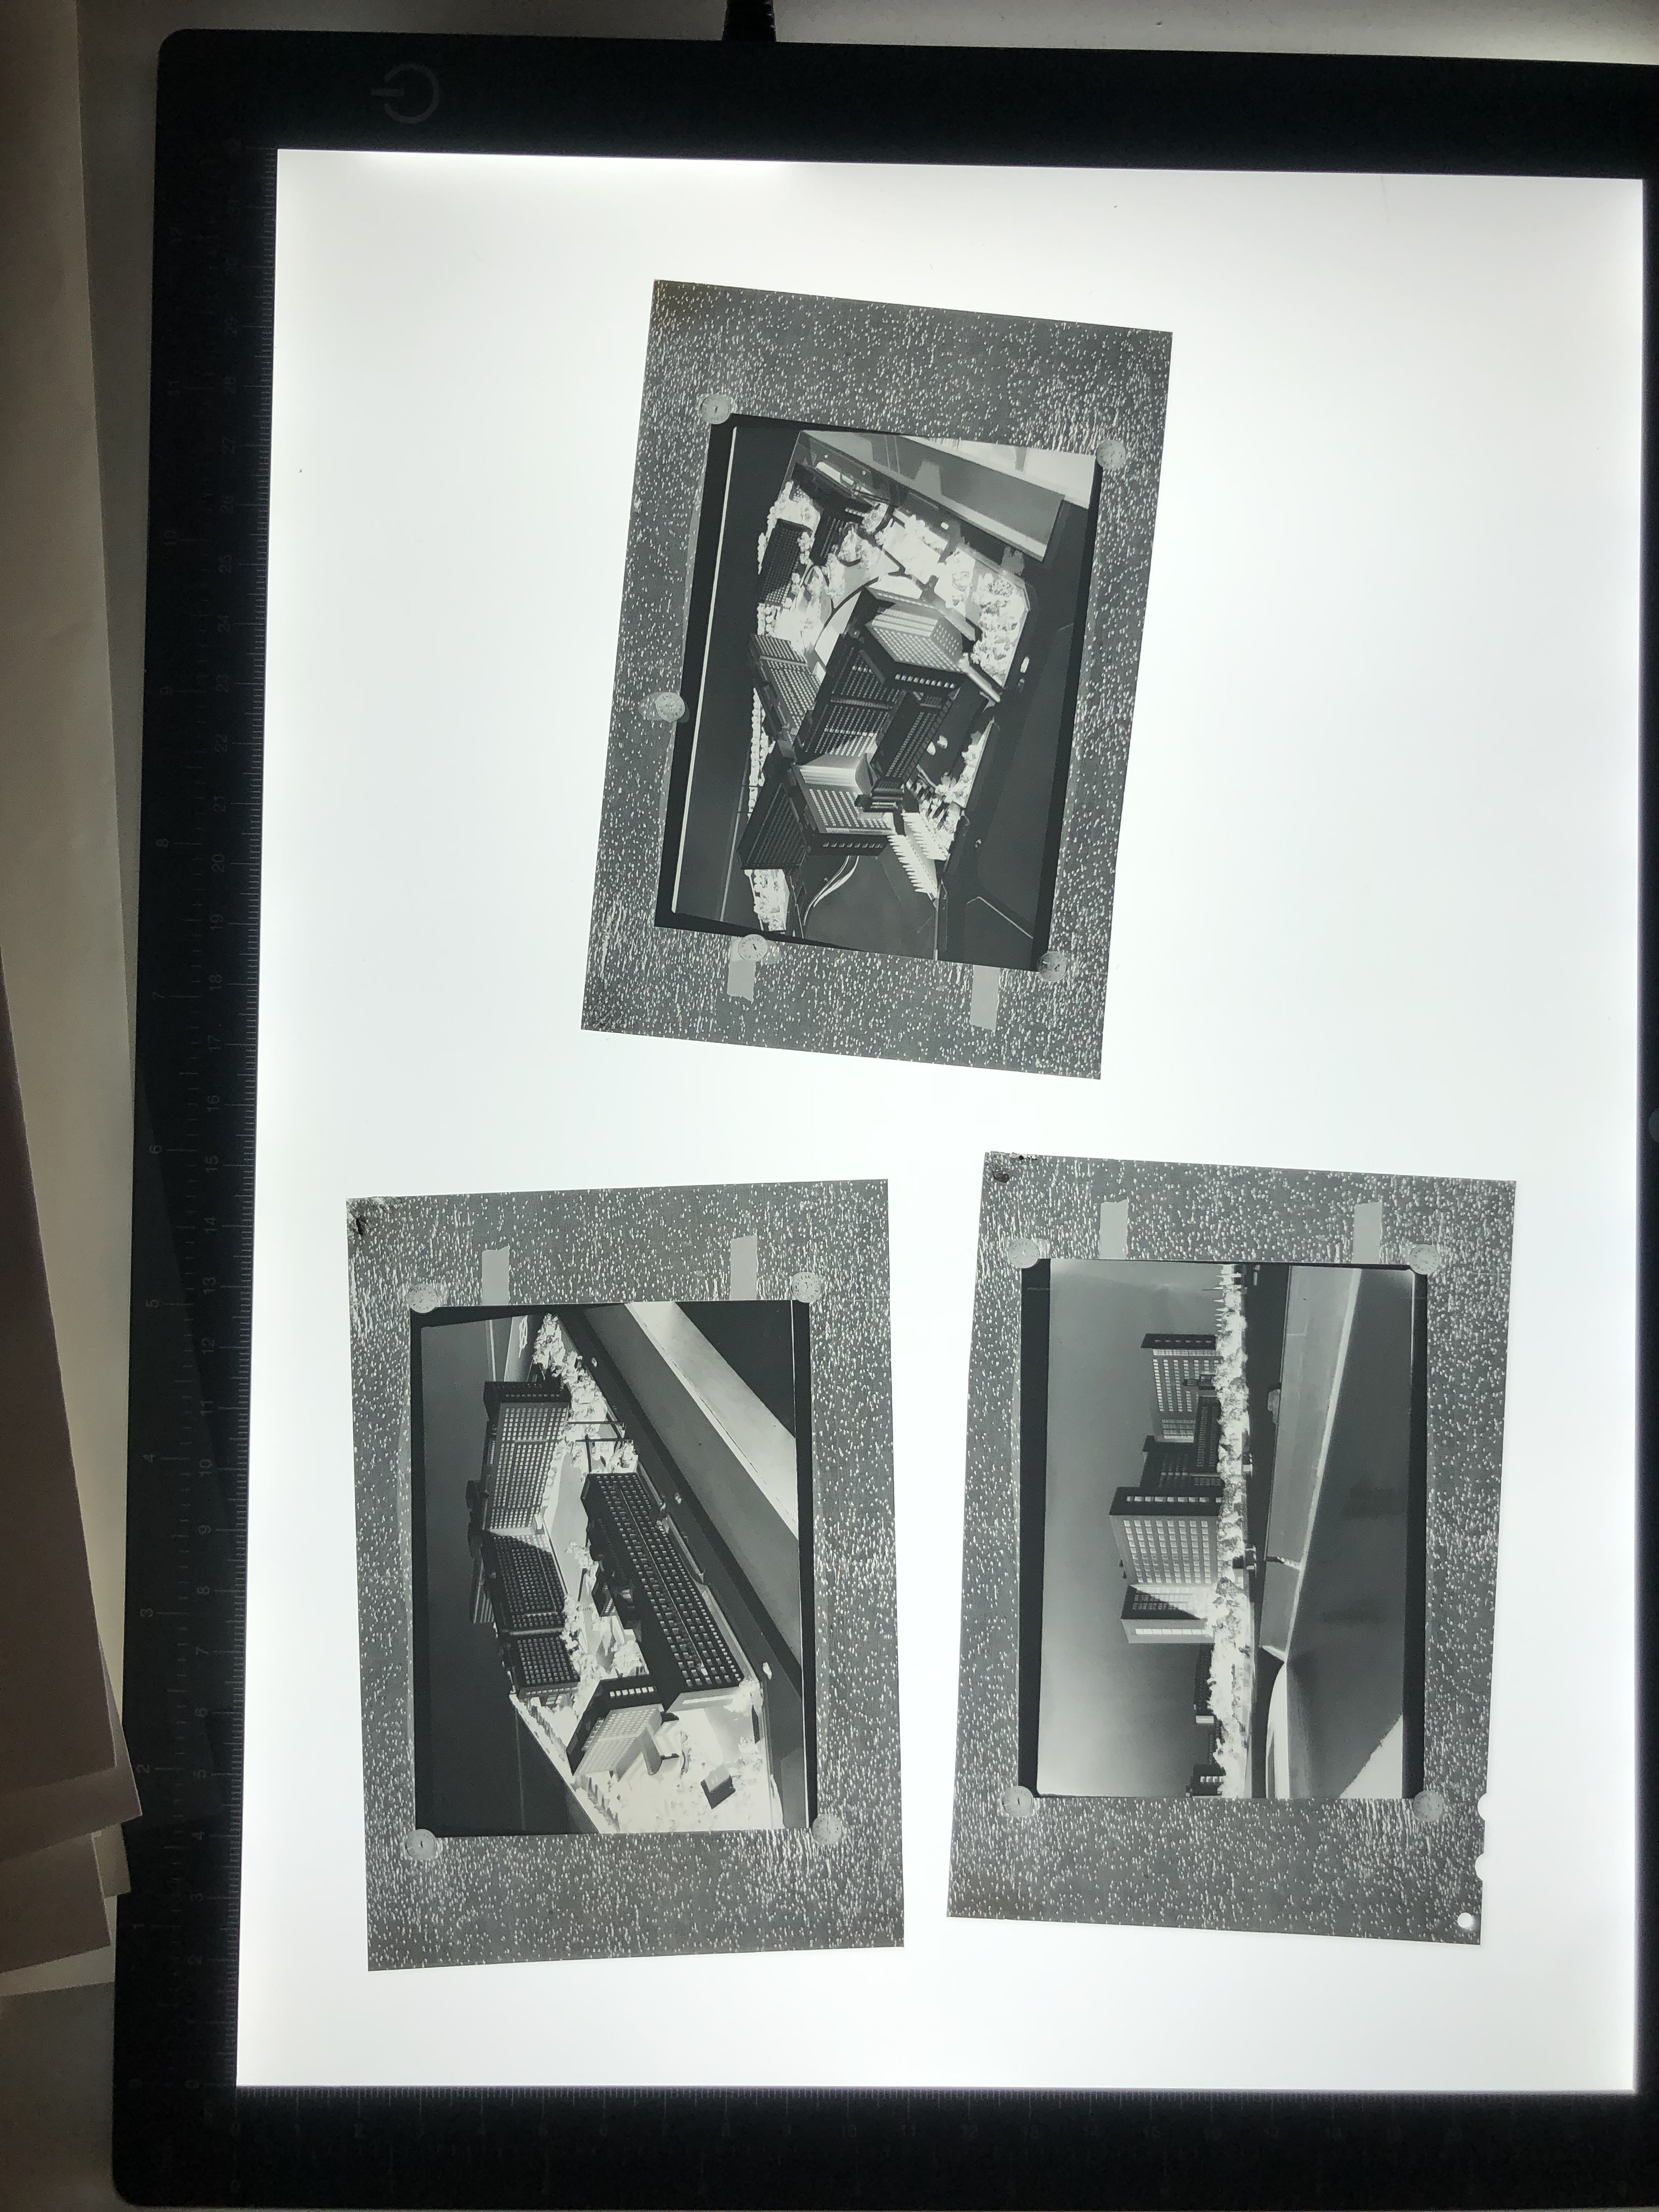
\includegraphics[width=\linewidth]{Illustrations/P12.jpg}
        \caption{}
    \end{subfigure}    
    \caption{Panorama des différents supports et formats d'images}
    \label{fig:pellicules}
\end{figure}    

Il y a plusieurs enjeux majeurs avec cette réalisation technique, tout d'abord le nommage des fichiers est en majeure partie un simple chiffre incrémenté de 1 en 1, n'offrant aucune information sur la bobine à laquelle appartenait la photo. Quelques rares photos comportent des noms de lieux, de commanditaires, des acronymes de sociétés, et l'idée sera de ne pas perdre cette information et qu'elle apparaisse dans le résultat final. Le premier enjeu est donc un enjeu de nomenclature des fichiers que nous allons produire en sortie, et donc de la réflexion que nous voulons avoir sur la manière de classifier ces objets. Le deuxième enjeu est celui des formats : il existe en tout 3 formats différents d'images, les jpg, les jpeg et les HEIC, qui sont le format produit sur iOS. Il va nous falloir harmoniser ces formats en perdant le minimum d'informations possible au moment des conversions. Enfin, troisième, et plus gros enjeu, la variété des images elle-même, comme illustrée dans l'échantillon que nous avons placé dans la page précédente. On trouve des bobines déroulées placées sur un appareil, des négatifs, des positifs, des photos développées, des plaques de verres, des supports sur tables rétroéclairées. Parfois, c'est une seule image qui apparaît, parfois c'est une image et des fragments des images précédentes et suivantes sur la bobine, parfois ce sont 3 à 6 images distinctes sur une prise de vue. De plus, l'angle des photos change en fonction du moment pendant la campagne de numérisation, on voit aussi parfois apparaître les gants de la personne qui manipule les acétates. Tout cela mis bout à bout nous donne déjà la feuille de route et les objectifs que notre code est censé accomplir.

Nous utilisons un script qui se sert de Florence-2 le Vision-language Model de Microsoft\footnote{\textit{cf}. le \textbf{\hyperref[sec:Glossaire]{Glossaire}} pour le terme \enquote{\textit{Vision-language Model}}, p.~\pageref{sec:Glossaire}.}. Sur le serveur JupyterHub du musée nous importons le corpus d'images, puis nous organisons en trois étapes le traitement dans un jupyter notebook. D'abord, faute de description, nous renommons toutes les images en incrémentant simplement de 1 en 1. Puis, nous passons un script pour uniformiser tous les formats d'images en .jpg. Enfin, nous faisons un prompt pour demander à Florence d'extraire et de créer des \textit{bounding box} autour de l'image ou des images qu'il détecte, de là en reprenant les coordonnées de ces \textit{bounding box}, nous automatisons le découpage des images pour les éclater en images individuelles\footnote{\textit{cf}. le \textbf{\hyperref[sec:Glossaire]{Glossaire}} pour le mot \enquote{prompt}, p.~\pageref{sec:Glossaire}.}. Enfin, un dernier traitement pourrait être possible : faire passer un OCR sur les images afin de récupérer des informations à même l'image pour tenter d'en donner une description minimale dans le titre de celle-ci. \hfill\break

\subsection{Le déploiement en conteneur docker de Panoptic}

Dans le cadre des ces mises en place d'outils, il a aussi fallu réfléchir à une manière de déployer sur plusieurs postes l'outil Panoptic du CERES. Dans le cadre du stage, le SI avait configuré un poste sous Ubuntu à notre attention, qui disposait des droits administrateurs. Cependant, c'est l'exception plutôt que la règle, et la plupart des employé\wokisme e\wokisme s du musée n'ont pas les droits administrateurs sur leurs machines. Dans un premier temps, nous avions envisagé d'installer une petite interface \textit{user-friendly} pour permettre aux employé\wokisme e\wokisme s de lancer l'application avec un simple double-clic sur un raccourci du bureau\footnote{\textit{cf}. le \textbf{\hyperref[sec:Glossaire]{Glossaire}} pour le terme \enquote{\textit{user-friendly}}, p.~\pageref{sec:Glossaire}.}. Autrement, Panoptic doit se lancer en ligne de commande, après l'installation d'un environnement virtuel et les employé\wokisme e\wokisme s ne se sentaient pas à l'aise de manipuler une invite de commande. En contournant cela par un raccourci, que nous venions directement installer sur l'ordinateur, cela épargnait au moins de recourir aux droits administrateurs pour l'installation, l'application et l'environnement virtuel étant configurés dans un dossier compressé. Le raccourci lançait simplement un court script en Python qui venait exécuter les commandes bash de manière transparente pour l'utilisateur et ouvrait Panoptic dans un navigateur web. 

Il reste que la solution posait deux problèmes majeurs. D'abord, l'ordinateur des employé\wokisme e\wokisme s devait être munis de Python, et pour cela les droits administrateurs étaient requis. Nous faisions donc appel au SI qui, à distance, autorisait l'installation, ce qui aurait pu représenter une perte de temps énorme s'il fallait déployer la solution à grande échelle. Deuxièmement, il fallait que les employé\wokisme e\wokisme s mettent en place eux-même le corpus qu'ils voulaient traiter en le copiant depuis la base sur la mémoire de leur ordinateur de travail, ce qui allait vite s'avérer intenable. \hfill \break

Grâce à la mise en place du serveur Jupyterhub, il a été possible de concevoir conjointement avec le SI, un déploiement de l'outil via l'intranet du musée. Un port http a été dédié au conteneur Docker contenant l'application Panoptic, ce qui le rendait accessible via une simple adresse URL à tous les postes connectés au réseau interne du musée. Il y avait donc une seule configuration unique à faire pour que tous\wokisme tes y aient accès. Aussi, cette conteneurisation du déploiement a permis de régler le second problème qui s'était posé : l'accès aux données du musée et le stockage. Le SI a pu monter directement en lecture seule les volumes de stockages principaux du musée. Cela permet de garder les arborescences que les employé\wokisme e\wokisme s connaissent déjà, et de ne pas avoir à dédoubler les données, en plus de permettre d'exporter les métadonnées que le personnel scientifique aura associé avec les bons chemins et numéros d'inventaire. 

Cependant, l'instance unique de Panoptic implique que tout le monde a accès aux projets des uns et des autres. L'idée de remonter à chaque fois un Docker avec les volumes en lecture etc,... serait trop chronophage pour le SI. Les concepteurs de l'outil n'avait pas pensé à faire un système de comptes, de log-in et de droits parce qu'ils n'en avaient pas l'utilité. Nous avons eu la chance de nous entretenir avec eux à propos de leur outil le 2 juillet 2025, notamment avec Édouard Brouté et Samuel Goncalves, afin de poser nos questions et de faire nos premiers retours sur les tests que nous avions déjà menés. Tout d'abord, le projet est un projet \textit{open-source} ce qui signifie que nous pourrions parfaitement implémenter un système d'authentification et de comptes pour remédier au problème de l'instance unique\footnote{\textit{cf}. le \textbf{\hyperref[sec:Glossaire]{Glossaire}} pour le terme \enquote{\textit{open-source}}, p.~\pageref{sec:Glossaire}.}. De plus, leurs explications étaient précieuses afin de mieux comprendre l'outil et certaines de ses limitations dans le domaine patrimonial. L'outil a été pensé pour des données nativement numériques, c'est-à-dire pour un objet image et non pour une chose photographiée. 

Ce point expliquera par la suite certains regroupements que fit l'outil pendant les tests où, par exemple, la disposition physique des objets pour des photos documentaires était jugée déterminante pour le rapprochement par similarité. C'est un point important pour le traitement de collections patrimoniales, mais un point qui peut être mitigé, ou bien même tourné à notre avantage grâce à une seconde caractéristique de l'outil : sa capacité à recevoir des plug-in et des modifications. Dans son architecture est pensée la possibilité d'ajouter des modules personnalisés, ce qui ouvre l'opportunité de brancher un modèle Clip entraîné spécifiquement sur des fonds patrimoniaux et des photos documentaires afin d'améliorer la pertinence des regroupements\footnote{\textit{cf}. le \textbf{\hyperref[sec:Glossaire]{Glossaire}} pour le terme \enquote{\textit{plug-in}}, p.~\pageref{sec:Glossaire}.}. Cela pourrait servir par exemple à repérer les dégradations, corrosions, déchirures et autres avaries sur les documents et les regrouper ensemble. Ils soulignent aussi que les étapes de tri et le processus itératif de description et caractérisation des images est indispensable parce que les premiers regroupements génèrent du bruit\footnote{\textit{cf}. le \textbf{\hyperref[sec:Glossaire]{Glossaire}}, p.~\pageref{sec:Glossaire}.} et le modèle apprend au fur et à mesure qu'on attribue des catégories à des images.

\section{Des outils d'IA aux mains des équipes}

Enfin, dans cette dernière partie, nous proposons la synthèse des entretiens que nous avons menés auprès de l'équipe des Arts graphiques autour de la manipulation de 3 outils d'intelligence artificielle\footnote{\textit{cf}. la \textbf{\hyperref[sec:Entretiens_2025]{Synthèse en Annexe C}}, p.~\pageref{sec:Entretiens_2025}.}. Ces entretiens ont été enregistrés entre juillet et août 2025, et reprennent une partie des conclusions et principes posés par la campagne d'entretien de décembre 2024 menés par Marion Charpier\footnote{\textit{cf}. la \textbf{\hyperref[sec:Entretiens_2024]{Synthèse en Annexe B}}, p.~\pageref{sec:Entretiens_2024}.}. Nous citerons les similitudes et conclusions concordantes des deux campagnes et nous réservons la partie propre aux entretiens de 2024 pour le prochain chapitre.

\subsection{Les outils présentés}

Pendant notre campagne d'entretien nous avons présenté 3 outils : \textit{Synesthesia}, Panoptic et Pixplot. \textit{Synesthesia} est un outil de rapprochement par similarité développé par Robert Erdmann Professeur à l'Université d'Amsterdam engagé par le MAD pour faciliter l'exploration des collections du musée. Le second, Panoptic, est un logiciel développé par le laboratoire CERES de Sorbonne Université\footnote{\cite{noauthor_ceres_nodate}.}. Le dernier est un outil développé par la \textit{Digital Humanities Lab} de l'Université de Yale\footnote{\cite{noauthor_yale_nodate}.}. Ces trois outils utilisent des technologies de clustering par similarité, mais pas toutes de la même époque. Le projet Pixplot date de 2017 et utilise Scikit-learn et TensorFlow\footnote{\textit{cf}. le \textbf{\hyperref[sec:Glossaire]{Glossaire}} pour les termes \enquote{Scikit-learn} et \enquote{TensorFlow}, p.~\pageref{sec:Glossaire}.}. Les deux autres utilisent Clip. 

\begin{figure}[H]
    \centering
    \begin{subfigure}{0.8\textwidth}
        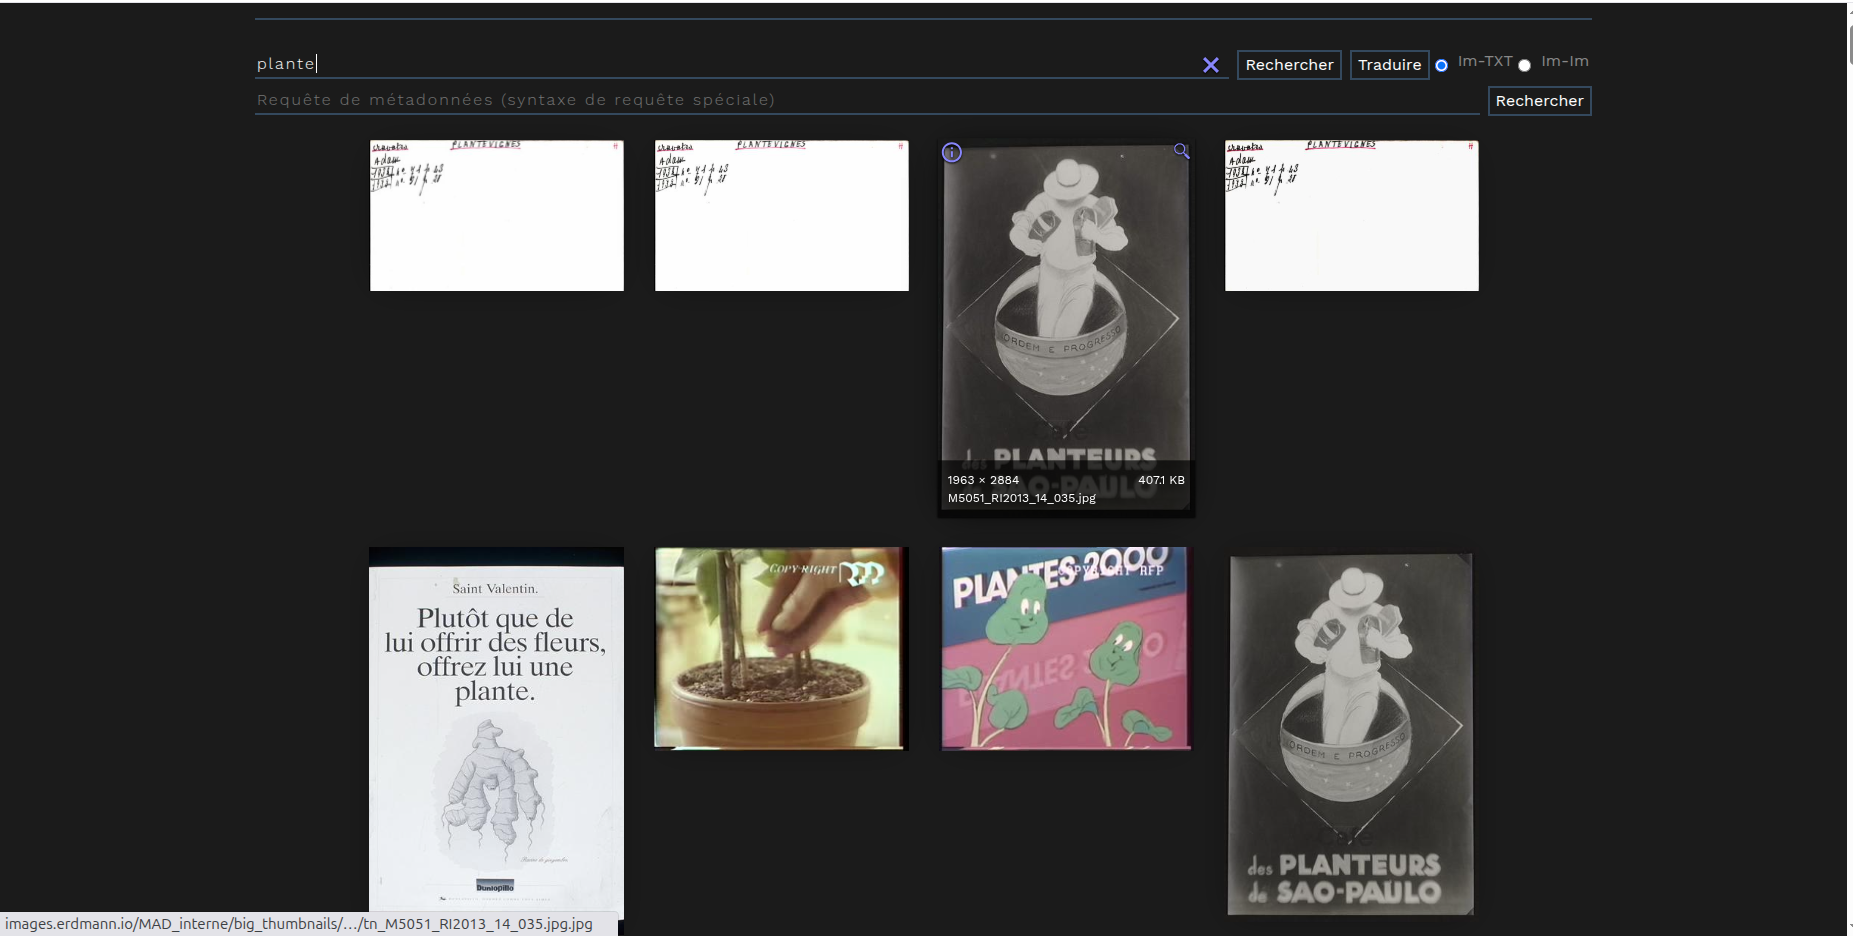
\includegraphics[width=\linewidth]{Illustrations/Synesthesia1.png}
        \caption{}
    \end{subfigure}
    \begin{subfigure}{0.8\textwidth}
        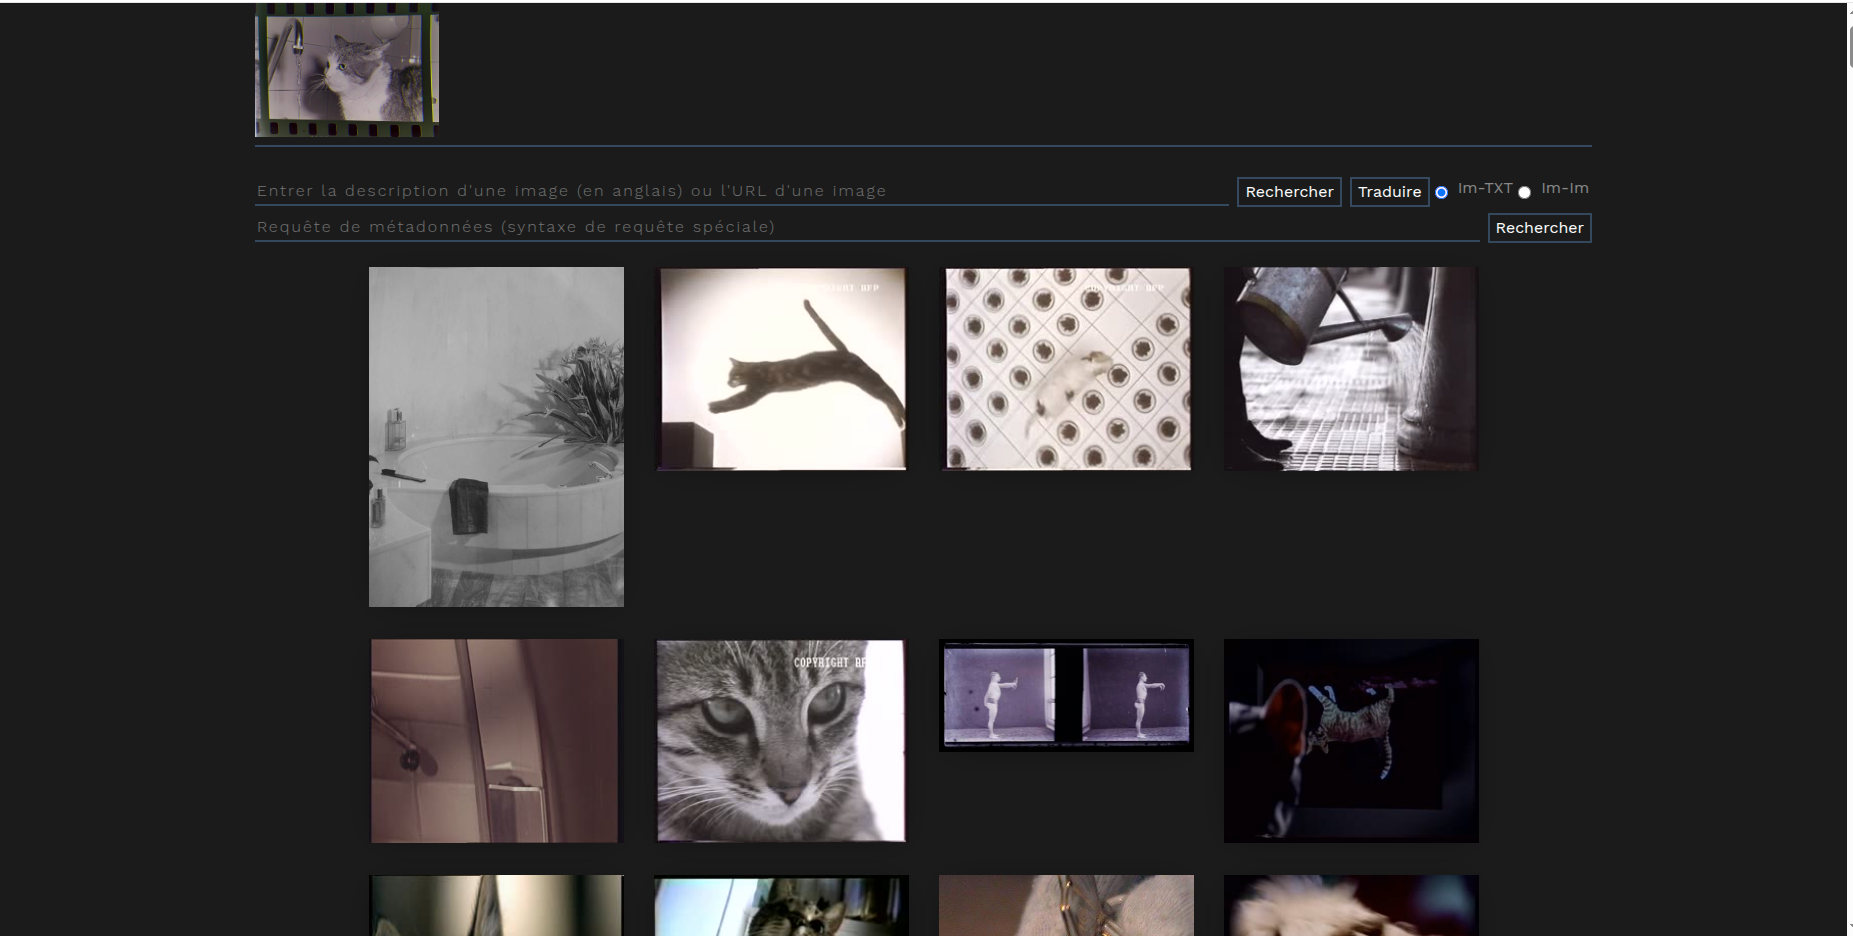
\includegraphics[width=\linewidth]{Illustrations/Synesthesia2.png}
        \caption{}
    \end{subfigure}
    \begin{subfigure}{0.8\textwidth}
        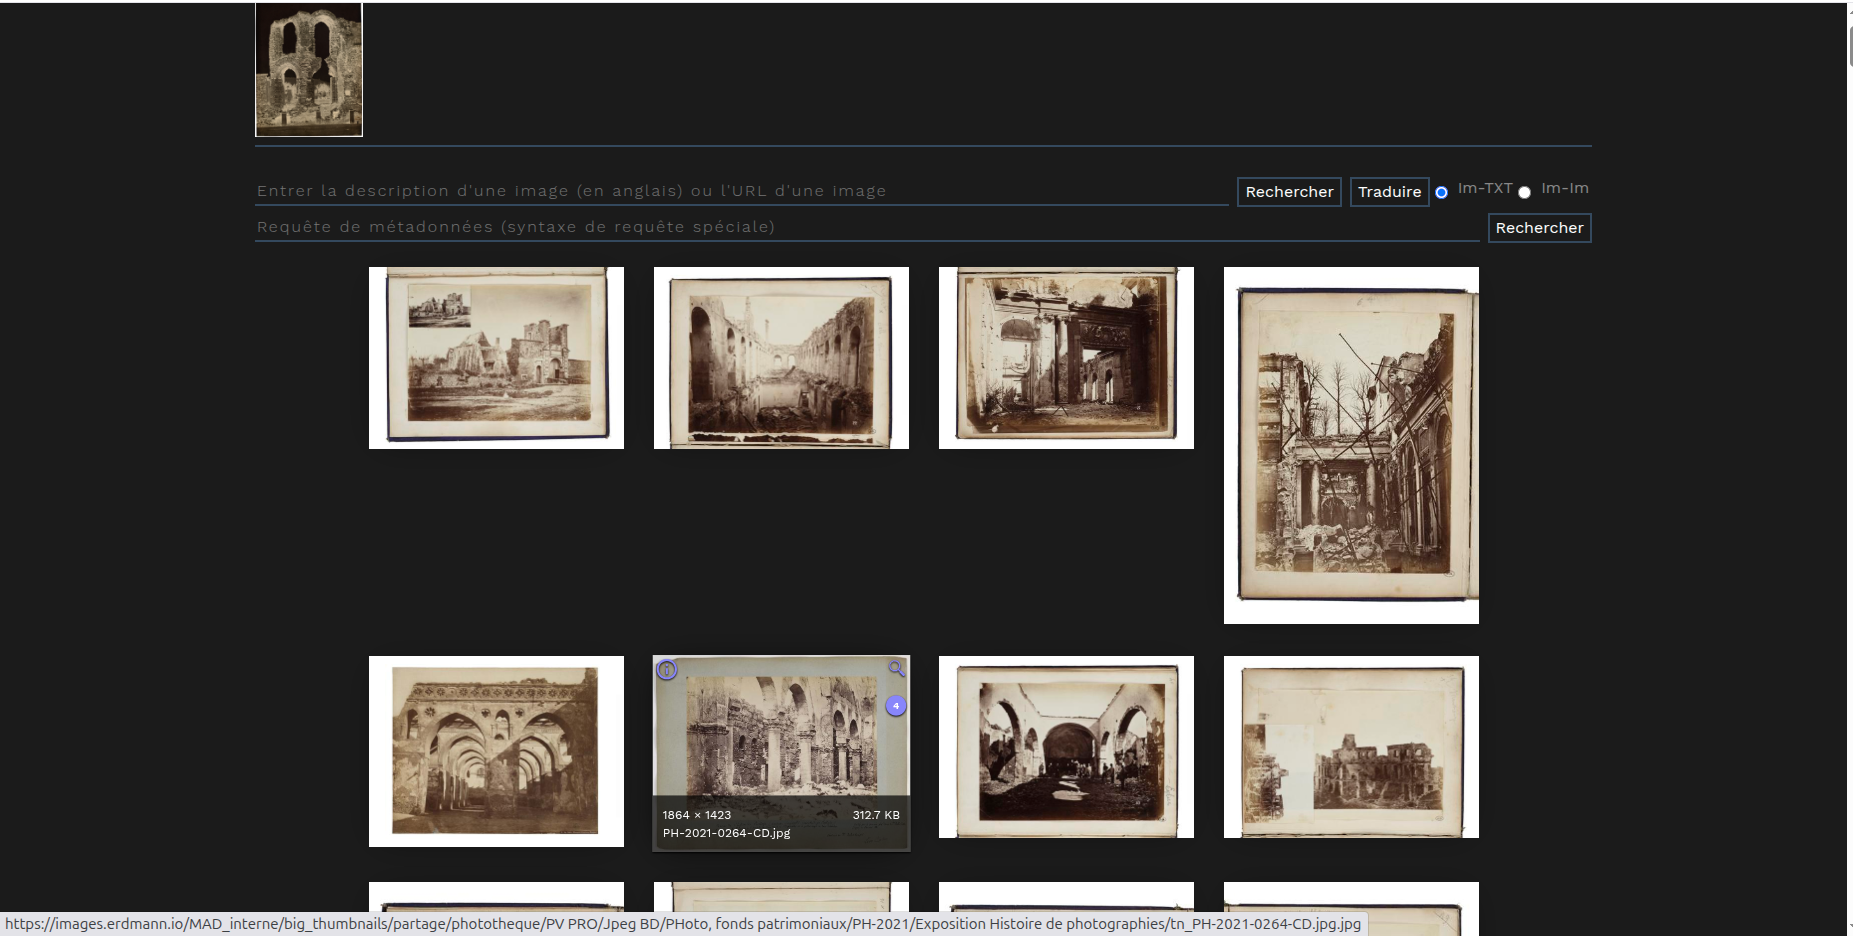
\includegraphics[width=\linewidth]{Illustrations/Synesthesia3.png}
        \caption{}
    \end{subfigure}
    \caption{Illustrations de \textit{Synesthesia}}
    \label{fig:pellicules}
\end{figure}    

Ici nous voyons quelques captures d'écrans qui illustrent le fonctionnement de \textit{Synesthesia}. L'outil consiste en un navigateur web dans lequel on peut faire des requêtes par texte, par image ou par métadonnées. L'outil est branché sur les bases du musée et montre tout ce qui est similaire ou qui correspond à la description écrite et qui se trouve dans les collections du musée. Lorsqu'on clique sur une image, l'application nous ouvre une fiche d'information qui contient le nom du fichier, son emplacement, sa taille et ses métadonnées associées. Si l’œuvre sur laquelle on clique figure dans la base de données Arcadie, alors cela nous redirige directement sur la fiche de l’œuvre dans la base. Dans les exemples donnés ici, nous avons d'abord fait une recherche par texte avec le mot \enquote{Plante}. Cette recherche nous montre autant des représentations de plantes que des documents contenant le mot recherché. Ensuite nous avons fait la recherche avec une numérisation d’œuvre qui n'est pas sur la base du musée, le chat près du robinet, et par similarité l'application a trouvé d'autres occurrences de chats dans les collections. Enfin, un négatif de photographie d'une collection qui se trouve dans les bases du musée et l'application nous a retrouvé les œuvres similaires, la plupart appartenant au même fonds.


\begin{figure}[H]
    \centering
    \begin{subfigure}{0.8\textwidth}
        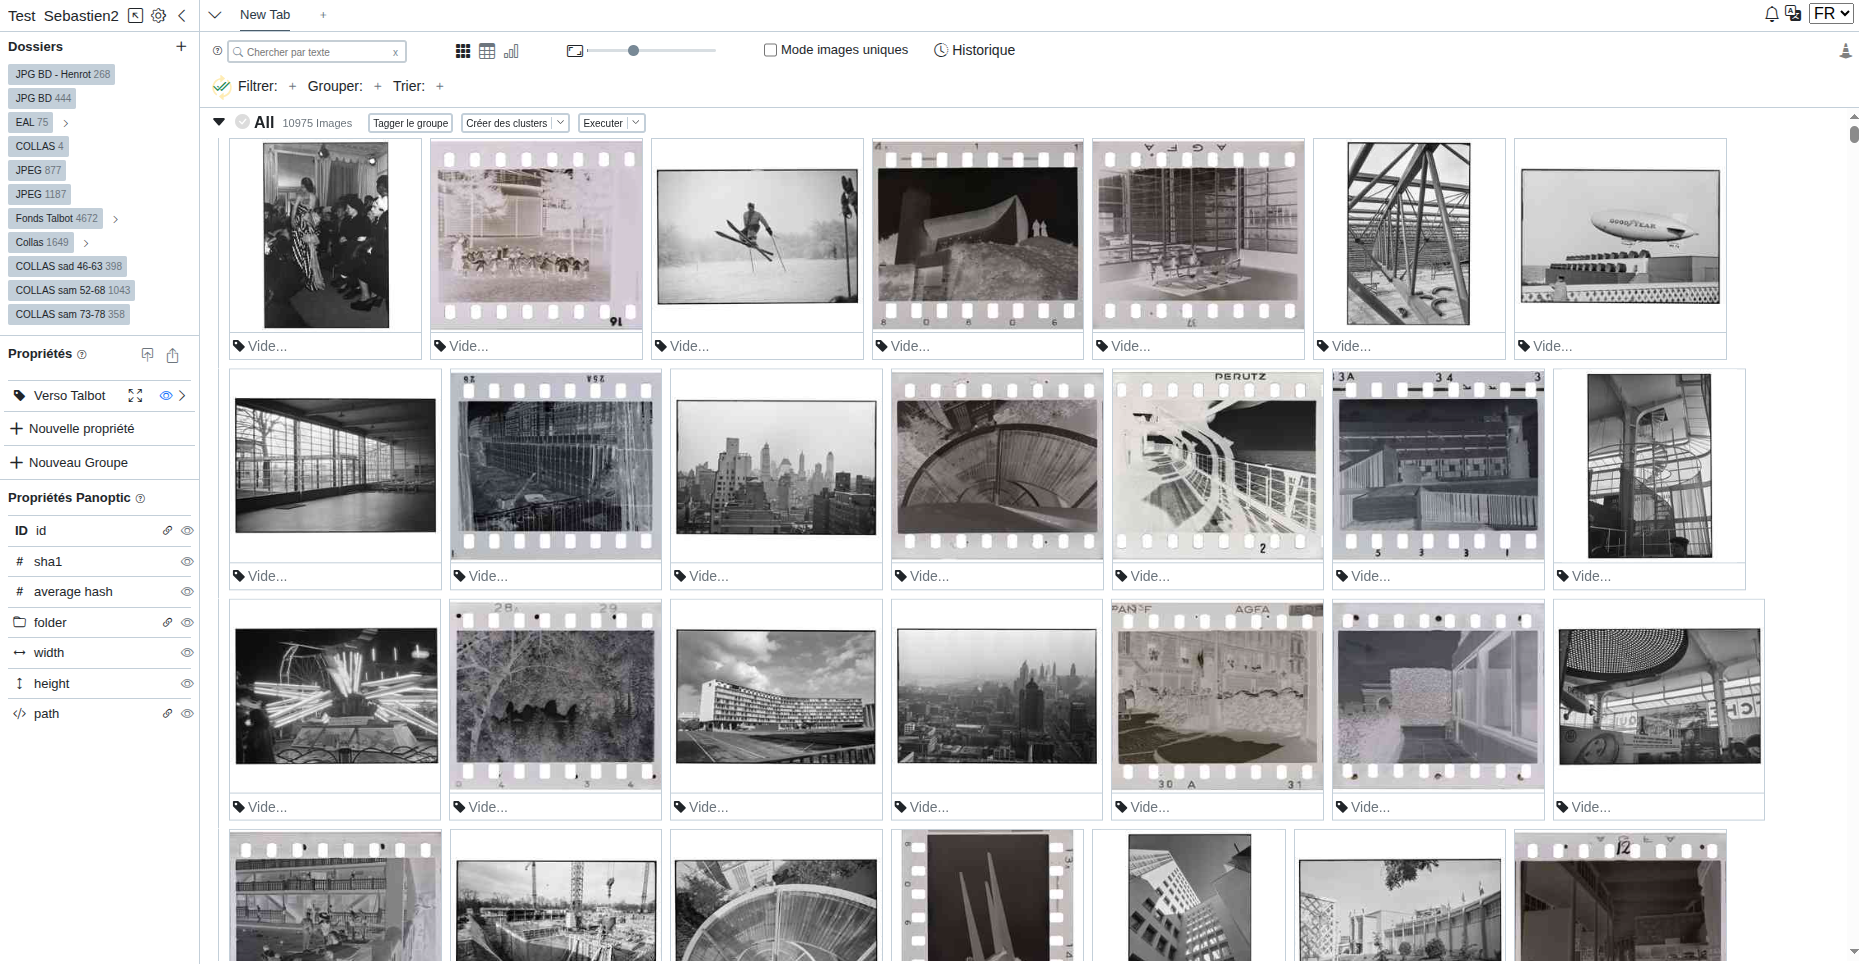
\includegraphics[width=\linewidth]{Illustrations/Panoptic1.png}
        \caption{}
    \end{subfigure}
    \begin{subfigure}{0.8\textwidth}
        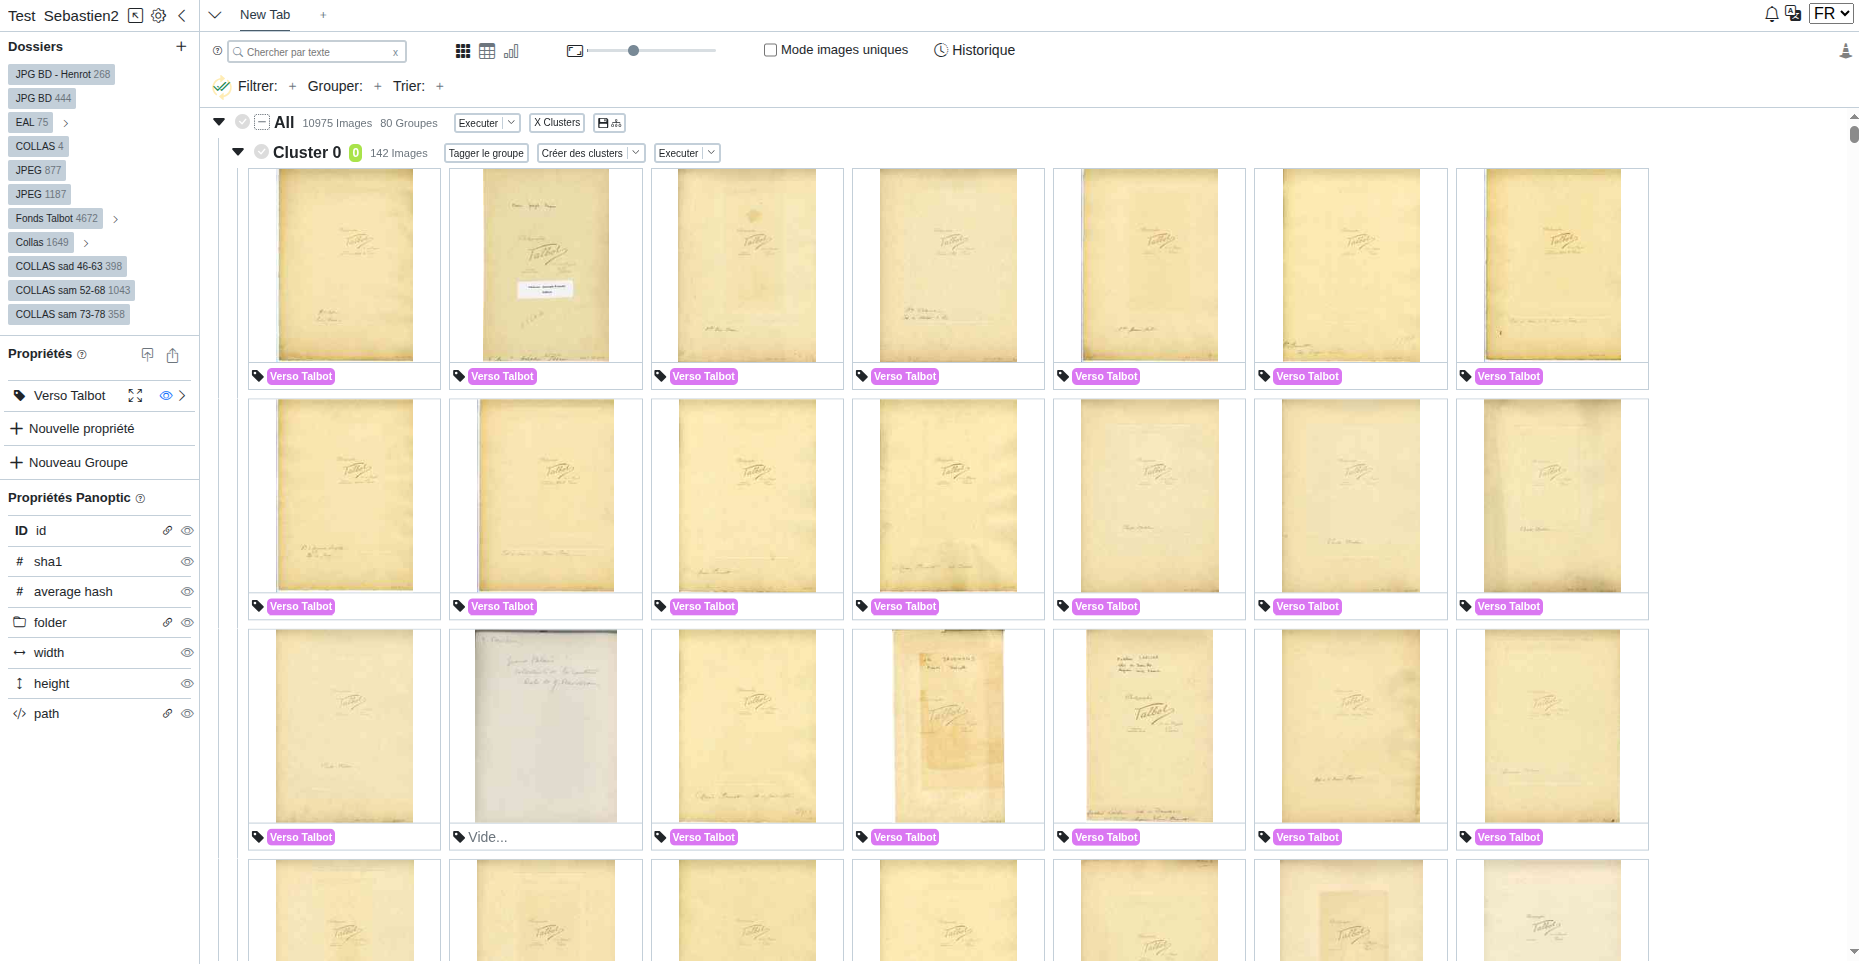
\includegraphics[width=\linewidth]{Illustrations/Panoptic2.png}
        \caption{}
    \end{subfigure}
    \begin{subfigure}{0.8\textwidth}
        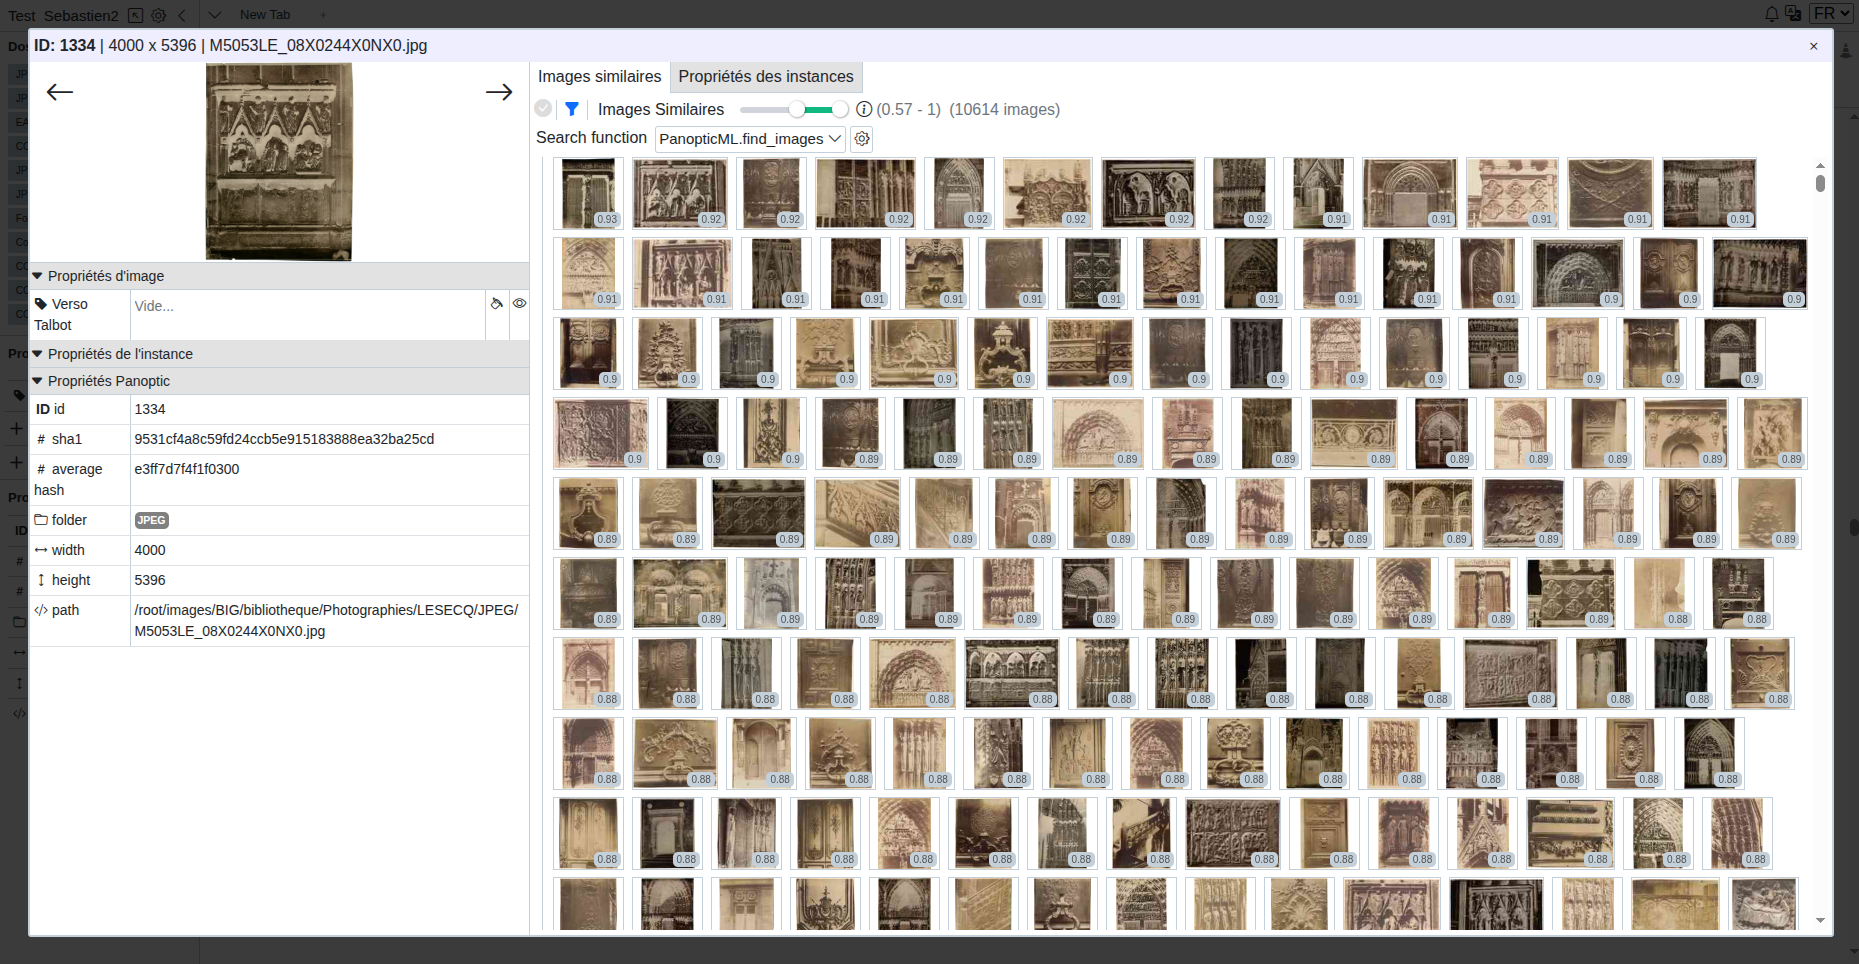
\includegraphics[width=\linewidth]{Illustrations/Panoptic3.png}
        \caption{}
    \end{subfigure}
    \caption{Illustrations de Panoptic}
    \label{fig:pellicules}
\end{figure}

De la même manière, le second outil est aussi une visionneuse d'image mais cette fois, dont le fonctionnement est différent. Ici on relie aussi les bases du musée à l'outil, on fait cependant une sélection dans les fonds puis on lance le regroupement par clusterisation. On donne à l'outil un certain nombre de regroupement à faire, imaginons 60, et il va créer des groupes avec des images qu'il pense similaire. Cet outil permet aussi de faire des recherches avec du texte, de générer les clusters en passant les images en niveau de gris. La démarche avec cet outil consiste à créer des étiquettes ou \textit{labels} et d'apposer des catégories aux images afin de décrire les œuvres. Il permet de trier, grouper ou filtrer les groupes que nous avons créés, afin de relancer la clusterisation en affinant les groupements et distinctions. La force de cet outil réside dans sa grande capacité d'absorption qui peut traiter 1 millions d'images dans un même projet, mais aussi dans la possibilité d'exporter en csv les métadonnées (les étiquettes) produites par l'agent. Cette fonctionnalité ouvre la possibilité de traiter les collections en masse, en s'aidant de la clusterisation et en gardant la maîtrise sur les données produites. Nous pouvons ainsi exporter les informations correspondantes grâce au fait que l'application garde aussi les chemins d'accès des fichiers en mémoire. Ceci évite l'écueil des mots-clefs générés par IA hors d'un vocabulaire contrôlé et qui peuvent s'avérer imprécis ou totalement erronés.


\begin{figure}[H]
    \centering
    \begin{subfigure}{0.8\textwidth}
        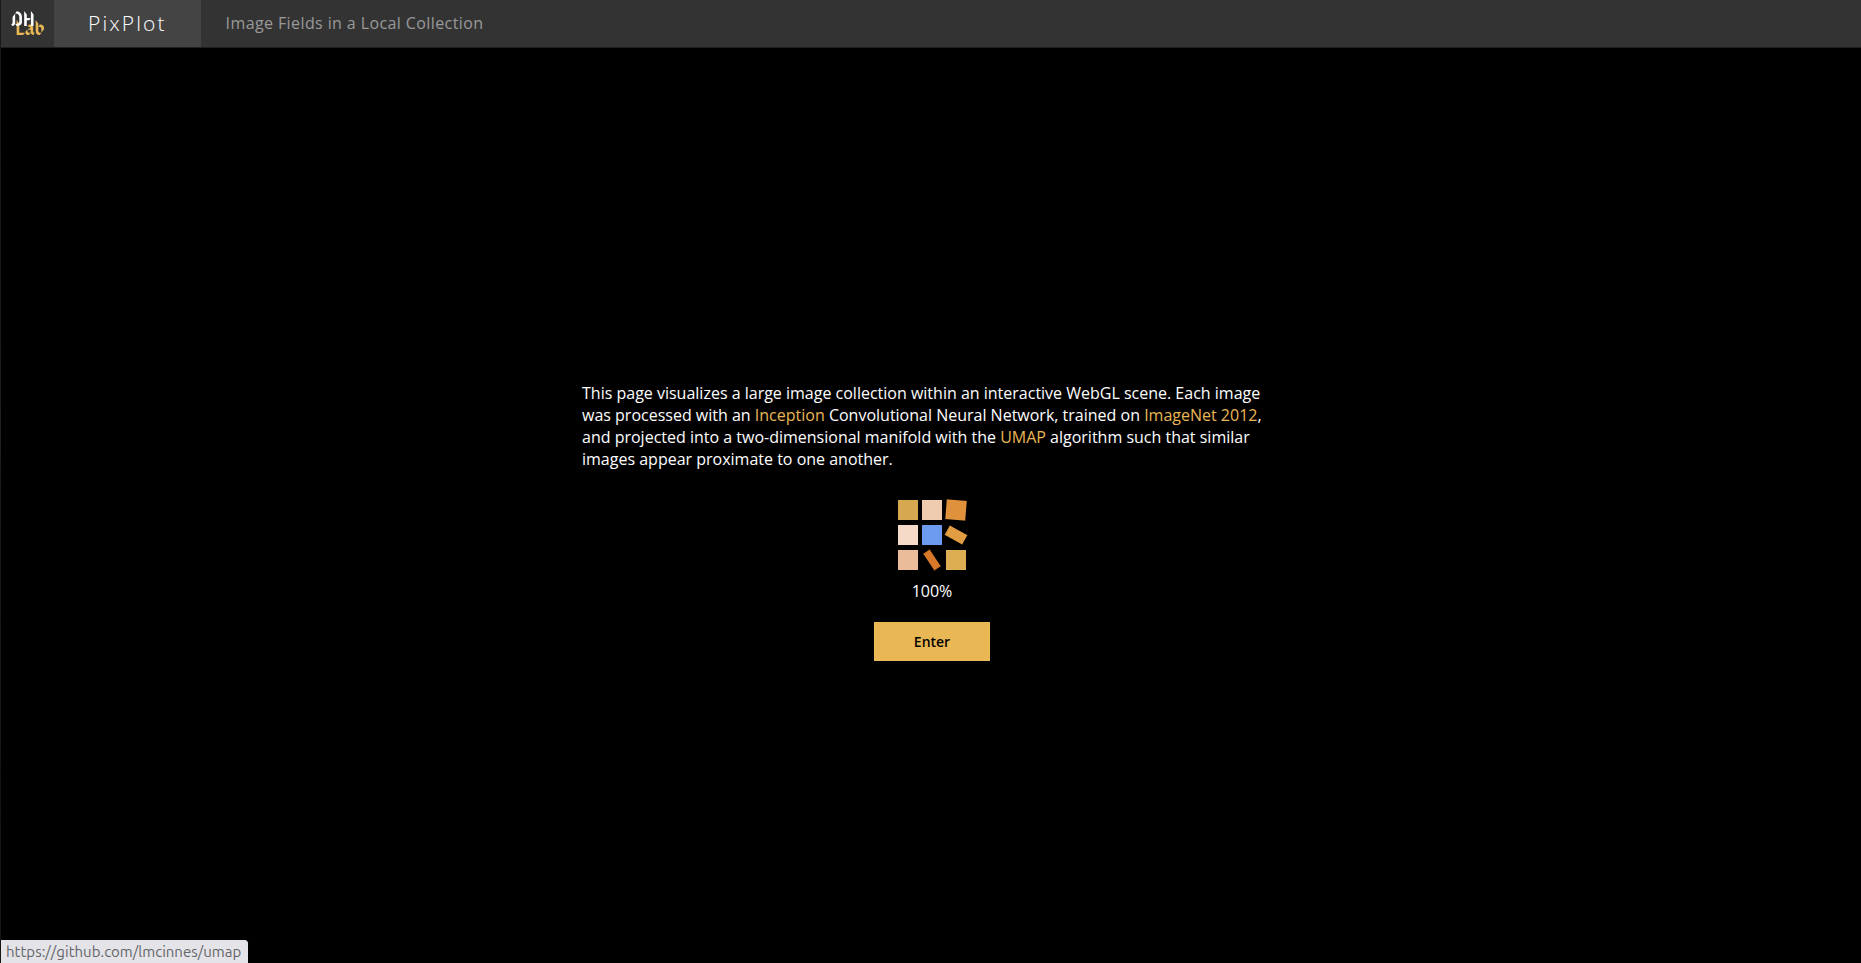
\includegraphics[width=\linewidth]{Illustrations/Pixplot1.png}
        \caption{}
    \end{subfigure}
    \begin{subfigure}{0.8\textwidth}
        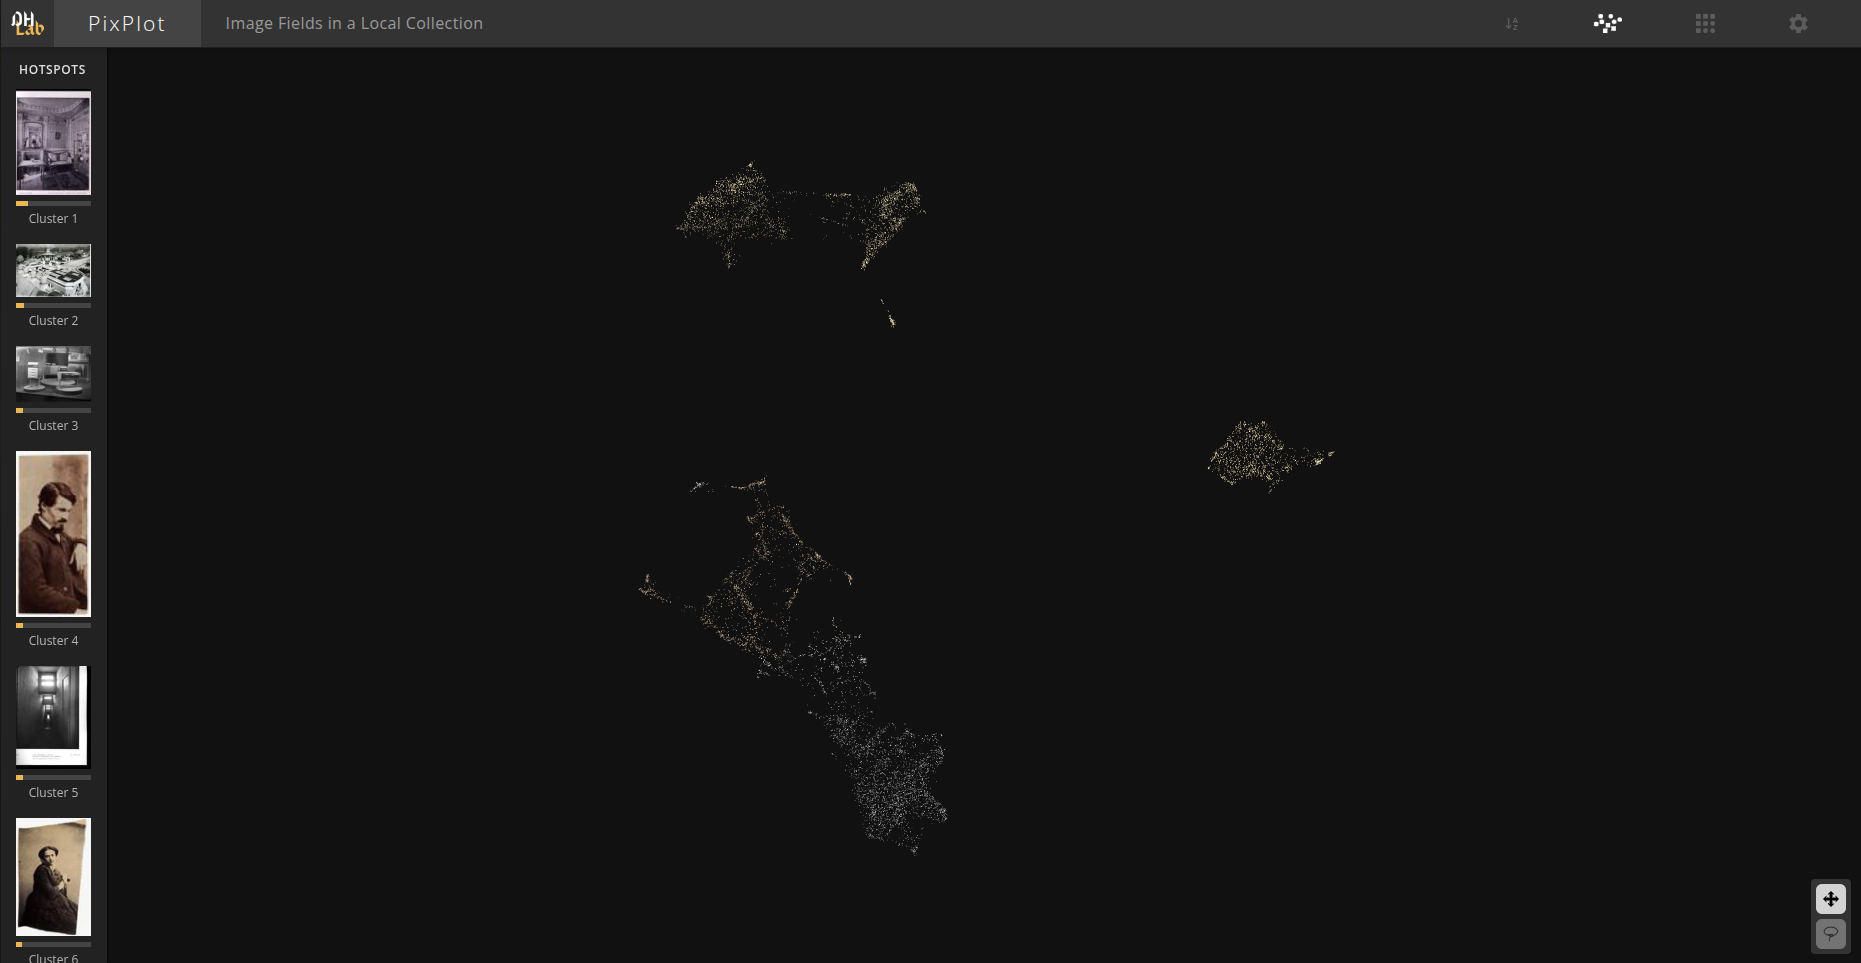
\includegraphics[width=\linewidth]{Illustrations/Pixplot2.png}
        \caption{}
    \end{subfigure}
    \begin{subfigure}{0.8\textwidth}
        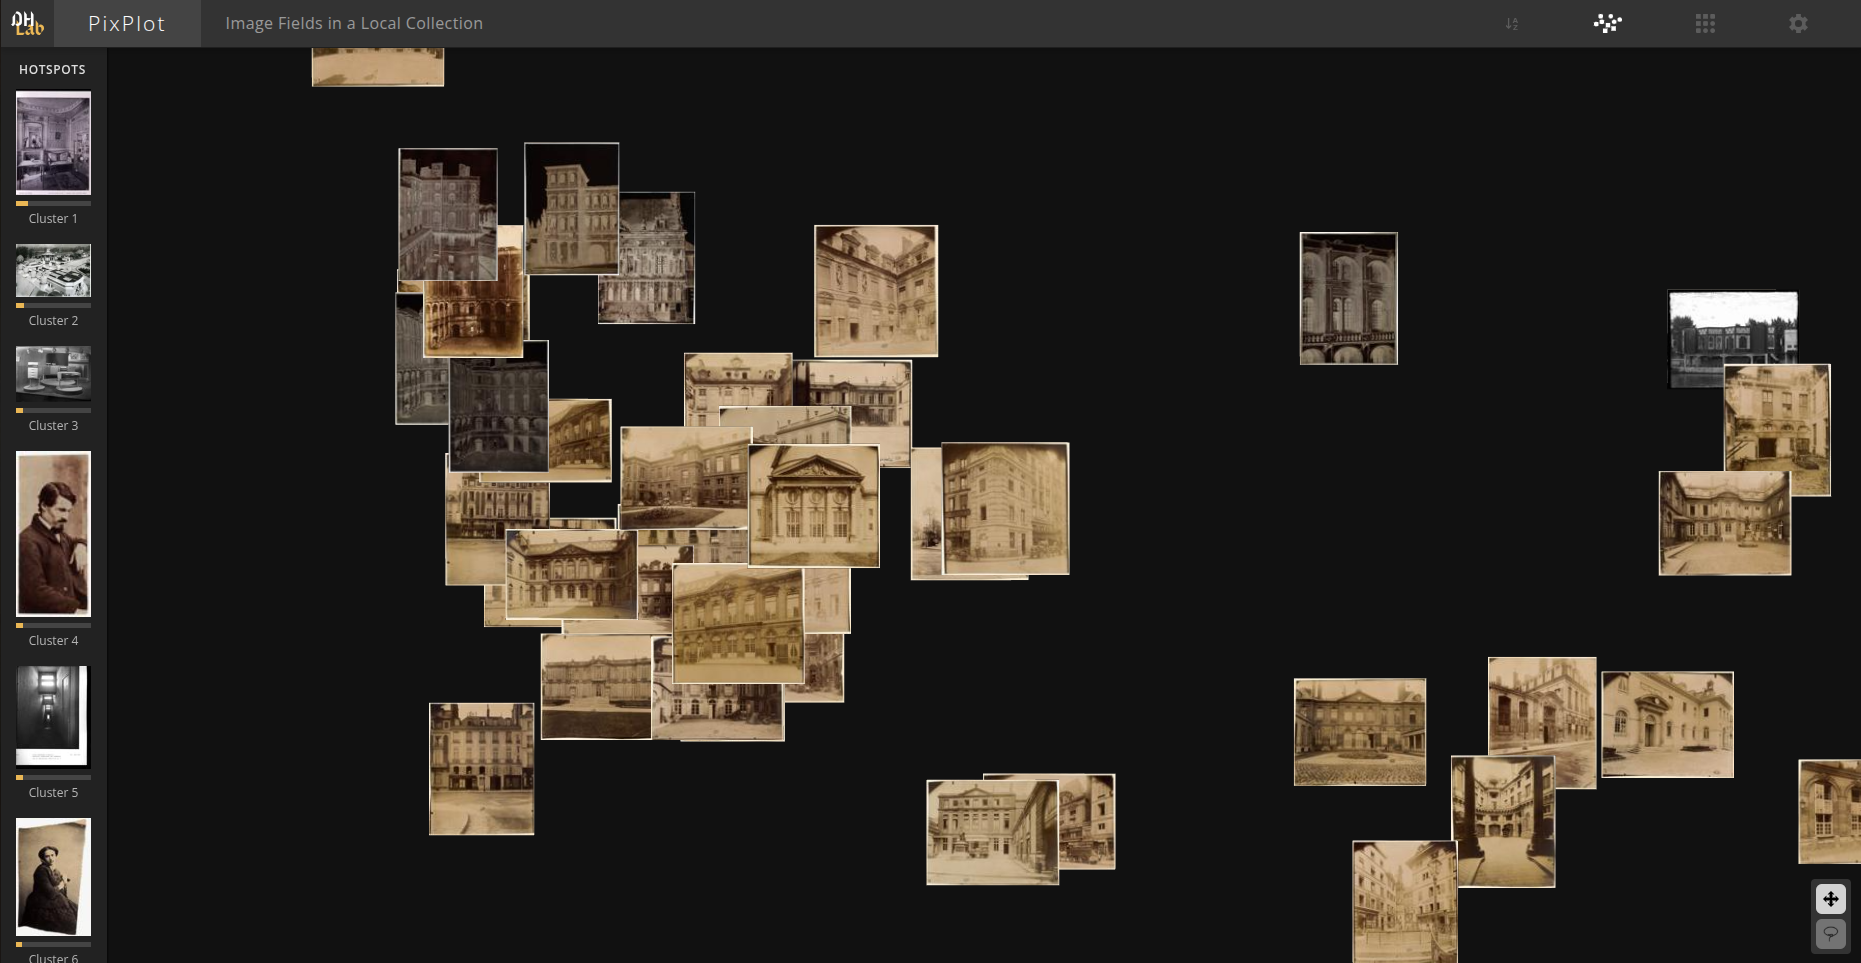
\includegraphics[width=\linewidth]{Illustrations/Pixplot3.png}
        \caption{}
    \end{subfigure}
    \caption{Illustrations de Pixplot}
    \label{fig:pellicules}
\end{figure}

Enfin, Pixplot qui est aussi un interface web et qui crée un carte en deux dimensions représentant les différences entre les images qu'on lui a fourni. C'est ce qui crée ces \enquote{continents} visuels qui rapproche les images des unes des autres ou les sépare en fonction de ce qu'elles représentent. Nous pouvons zoomer, retrouver les noms des fichiers et cliquer sur les images pour les agrandir. Cependant, l'application n'est pas reliée aux bases du musée, ce qui empêche d'avoir les chemins d'accès complet vers les dossiers où les images sont stockées.

\subsection{Le résultat des prises en main}

C'est donc l'utilisation de ces 3 outils-là que nous avons évalué au sein des équipes du département des Arts graphiques. La conduite des entretiens s'est déroulée entre juillet et août 2025 et ont tous fait l'objet d'une captation sonore et vidéo. Pour la transcription, nous avons eu recours à l'outil EchoInStone qui est un logiciel utilisant Whisper, logiciel de transcription développé par OpenAI, et qui ajoute une couche de diarisation au résultat\footnote{\cite{levy_jeanjeromeechoinstone_2025}}. Nous avons installé le logiciel sur le serveur JupyterHub du musée afin de pouvoir tirer profit des infrastructures, et spécifiquement du GPU du musée. Nous voulions la meilleure transcription possible donc nous avons lancé le modèle large pour chaque entretien, ce qui a demandé une puissance de calcul et un temps considérable qu'il n'aurait pas été possible de mobiliser avec notre ordinateur professionnel. 

Chaque outil remplit un rôle différent aux yeux des équipes et nous allons reprendre le résultat de ces prises en main ici. Nous avons, par ailleurs, produit une synthèse des entretiens qui se trouve en Annexe C\footnote{\textit{cf}. l'\textbf{\hyperref[sec:Annexe C]{Annexe C}}, p.~\pageref{sec:Entretiens_2025}.}. Tout d'abord \textit{Synesthesia} permet de raccourcir considérablement les temps de recherches dans l'inventaire et sur les bases du musée. Le cas d'usage le plus courant est celui où un\wokisme e chercheur\wokisme euse ou un particulier demande de retrouver un papier peint, un dessin ou une photographie dans les collections qu'il ou elle a pris en photo lors d'un passage au musée. Dans ce cas, l'outil est très pratique parce qu'il est relié autant à la base de données Arcadie du musée, qu'aux serveurs où se trouve l'ensemble de la production antérieure à la migration vers la base. Par similarité, l'outil retrouve l’œuvre dans les collections et indique combien il existe d'exemplaires de la même représentation d’œuvre, ses formats différents, ses emplacements. L'autre point soulevé lors des entretiens est l'aspect d'exploration que permet l'outil. En mettant une image de quelque chose de ressemblant, les personnels du musée peuvent aussi se laisser porter en explorant ce que l'outil trouve et être surpris, découvrir de nouvelles choses dans les collections, de nouvelles associations qui n'existent pas dans la base de données, etc,. Cependant l'outil reste limité en terme de cas d'usages à certains égards. En effet, la moitié des personnes sondées ne l'utilisent pas ou ne l'ont utilisé qu'une fois il y a longtemps. Les résultats peuvent s'avérer imprécis, l'outil produit du silence et l'instantanéité des résultats empêche paradoxalement l'exploration et la connaissance des fonds par tâtonnement. Aussi, l'outil met trop d'emphase sur les couleurs pour déterminer la similarité ou dissimilarité entre des images, là où, dans les cas d'usages, la question des motifs revient beaucoup plus souvent. Enfin, la recherche par texte est très peu utilisée et la recherche par métadonnées n'était pas connue des équipes. En général, l'outil est très utile pour les personnes qui s'en servent même s'il comporte des limitations.

Ensuite, en ce qui concerne Panoptic, la majorité des personnes interrogées s'est déclarée favorable à l'introduction de l'outil dans sa routine de travail. Les points en faveur de cette introduction qui sont ressortis après les manipulations sont les suivants : l'outil est rapide, il propose des regroupements indépendants d'un pré-traitement, il permet de guider la réflexion, de s'orienter dans un fonds mal connu, de requêter par texte, d'étiqueter les données et d'exporter ces étiquettes dans un csv avec les chemins de fichiers associés aux étiquettes, mais aussi de traiter les images en niveau de gris pour mitiger l'impact de la couleur sur les regroupements. Enfin, il permet de passer en revue une grande quantité d'image grâce à sa présentation sous forme de vignette et la facilité d'utilisation du zoom. Ce qui est ressorti est que pour caractériser un fonds défini, l'outil pourrait être très précieux, il est peut-être moins indiqué pour les recherches plus généralistes comme \textit{Synesthesia} en est capable. Quelques points négatifs ont été soulevés cependant, notamment certains regroupements hasardeux produits par l'outil qui ne semblaient pas faire sens pour le personnel, la possibilité de ne rechercher par texte qu'en anglais et le manque de compréhension des images. Ce dernier point vient du fait que l'outil a été pensé pour des images nativement numériques et non des photographies de supports ou d’œuvres. Ceci a pour effet de surdéterminer la similarité sur la base de la présentation physique des objets dans les photos (le même angle, la même lumière, la même table sur laquelle sont posées les œuvres) plutôt que sur le contenu, c'est-à-dire l’œuvre. Cependant, cette limitation peut être mitigée par la possibilité qu'offre l'outil d'y ajouter un plug-in avec par exemple un modèle Clip ré-entraîné qui se concentrerait plus sur les œuvres et moins sur le contexte des images. Dans l'ensemble, l'outil apparaît utile pour l'exploration et le traitement des collections, mais pas pour la médiation auprès d'un\wokisme e chercheur\wokisme euse ou du public.

Enfin, Pixplot semble être un outil intéressant pour la majorité des personnes sondées. Cependant, ils et elles précisent bien que c'est plus dans l'optique d'une première approche ou d'une visualisation très large d'un fonds qu'on ne connaît pas ou peu. Les personnes estiment que les rapprochements thématiques sont efficaces, bien que certaines anomalies et associations marginales dans les \enquote{continents} relèvent de l'erreur d'interprétation du modèle. Par exemple, les rapprochements des motifs de papiers peints étaient plus justes dans cet outil que dans Panoptic. La présentation de l'outil est esthétiquement agréable et intuitive, ce qui offre une belle première approche d'un fonds ou d'une collection de fonds. Il faut noter néanmoins, que l'impossibilité de retravailler les clusters après un premier résultat est très limitante. En général, pour l'exploration et la médiation des collections, l'outil est jugé adapté. En revanche, pour la description des collections, il ne convient pas.

\chapter*{Conclusion}

Cette partie se voulait être autant un compte-rendu du travail accompli, qu'un panorama de ce qui existe dans et autour du projet. Nous avons pu explorer la galaxie d'institutions et d'initiatives qui entourent l'entrée des humanités numériques utilisant l'IA dans les musées et le patrimoine. Nous avons aussi rendu compte des difficultés techniques, parfois organisationnelles, qui ont entourés les productions que nous avions à fournir. Nous avons pu aussi faire un premier bilan de l'introduction de l'IA au cœur d'un département de conservation. À notre sens, ce qui apparaît à l'aune de ces développements, c'est tout d'abord les opportunités et l'effervescence qui entourent ce domaine, mais aussi, en creux, l'autre face de ce genre de projets. En effet, si les opportunités sont nombreuses, les difficultés le sont tout autant. L'acculturation des équipes, les infrastructures, les limitations techniques, les spécificités des fonds, et bien d'autres domaines encore sont des points d'attention que nous devons garder à l'esprit face à la demande croissante de recours à ce genre de procédés. Depuis l'entrée de l'Intelligence Artificielle dans l'imaginaire du grand public, à la faveur de la sortie de ChatGPT le 30 novembre 2022, la notion d'IA exerce un formidable pouvoir d'attraction sur les individus comme les institutions, qui veulent s'emparer des nouvelles possibilités offertes par ces outils. Ce pouvoir d'attraction s'accompagne de réserves aussi, de la part de certain\wokisme e\wokisme s, mais aussi de certaines de confusions ou d'attentes démesurées vis-à-vis de l'outil. C'est tous ces points que se propose de traiter le prochain mouvement de ce travail, qui va s'attacher à pointer les limites, à souligner les opportunités et à proposer un certain nombre de manières d'introduire l'IA, de manière pérenne, au musée des Arts décoratifs, et plus largement dans les institutions patrimoniales françaises.